\documentclass[conference]{IEEEtran}

% b for integer/boolean values?
% Change notation - state vs disturbance/external input/uncontrolled input - but could these also be classified as states and disturbance/external input/uncontrolled input are subcategorisations of states?

% Packages
\usepackage{algorithmic}
\usepackage{amsfonts}
\usepackage{amsmath}
\usepackage{amssymb}
\usepackage{auto-pst-pdf}
\usepackage{booktabs}
\usepackage{bm}
\usepackage{cite}
\usepackage{dirtytalk}
\usepackage{etoolbox}
\usepackage{fixmath}
\usepackage{glossaries}
\usepackage{graphicx}
\usepackage[bookmarks=true]{hyperref}
\usepackage{ifthen}
\usepackage[utf8]{inputenc}
\usepackage{lipsum}
\usepackage{multicol}
\usepackage[numbers]{natbib}
\usepackage{nomencl}
\usepackage{psfrag}
\usepackage{pstool}
\usepackage{siunitx}
\usepackage{textcomp}
\usepackage{tikz}
\usepackage{unicode-math}
\usepackage{xcolor}
\usepackage{xfrac}

\makenomenclature
\makeglossaries

% Nomenclature categories
\renewcommand{\nomgroup}[1]{%
% Acronyms
\ifthenelse{\equal{#1}{A}}{\item[\textbf{Acronyms}]}{}
% Subscripts
\ifthenelse{\equal{#1}{B}}{\item[\textbf{Subscripts}]}{}
% Constants
\ifthenelse{\equal{#1}{C}}{\item[\textbf{Constants}]}{}
% Superscripts
\ifthenelse{\equal{#1}{P}}{\item[\textbf{Superscripts}]}{}
% Sets
\ifthenelse{\equal{#1}{S}}{\item[\textbf{Sets}]}{}
% Variables
\ifthenelse{\equal{#1}{V}}{\item[\textbf{Variables}]}{}

% % Other options
% \ifthenelse{\equal{#1}{R}}{\item[\textbf{Roman}]}{}
% \ifthenelse{\equal{#1}{G}}{\item[\textbf{Greek}]}{}
}

% atan2 operator
\DeclareMathOperator{\atantwo}{atan2}
% Nomenclature units
\newcommand{\nomunit}[1]{%
\renewcommand{\nomentryend}{\hspace*{\fill}#1}}

% Other
\def\BibTeX{{\rm B\kern-.05em{\sc i\kern-.025em b}\kern-.08em
    T\kern-.1667em\lower.7ex\hbox{E}\kern-.125emX}}
    
\tikzset{every picture/.style={line width=0.75pt}} %set default line width to 0.75pt

\begin{document}

\title{Integrated Model Predictive Fuzzy Control for Disaster Victim Detection Path Planning}

\author{\IEEEauthorblockN{Craig Maxwell}
\IEEEauthorblockA{\text{Department of Control \& Simulation, Aerospace Engineering} \\
\textit{Delft University of Technology}\\
Delft, The Netherlands \\
\href{mailto:hello@craigmaxwell.me}{hello@craigmaxwell.me}, \href{mailto:cmaxwell@student.tudelft.nl}{cmaxwell@student.tudelft.nl}
\and
\IEEEauthorblockN{2\textsuperscript{nd} Dr Anahita Jamshidnejad}
\IEEEauthorblockA{\text{Department of Control \& Simulation, Aerospace Engineering} \\
\textit{Delft University of Technology}\\
Delft, The Netherlands \\
A.Jamshidnejad@tudelft.nl}
}
}

\maketitle

\begin{abstract}
    \lipsum[2-4]
\end{abstract}
% TO DO: complete

\begin{IEEEkeywords}
MPC, Fuzzy Control, Path Planning, Search and Rescue
\end{IEEEkeywords}

% Nomenclature
\nomenclature[A]{2D}{Two Dimensional}
\nomenclature[A]{3D}{Three Dimensional}
\nomenclature[A]{FIS}{Fuzzy Inference System}
\nomenclature[A]{GIS}{Geographic Information System}
\nomenclature[A]{MF}{Membership Function}
\nomenclature[A]{MPC}{Model Predictive Control}
\nomenclature[A]{MPFC}{Model Predictive Fuzzy Control}
\nomenclature[A]{RNG}{Random Number Generator}
\nomenclature[A]{SAR}{Search-and-rescue}
\nomenclature[A]{TSK}{Takagi-Sugeno-Kang}
\nomenclature[A]{UAV}{Unmanned Aerial Vehicle}

% Unsorted
\nomenclature[]{$p(t_{\text{bt}})$}{Indoor standard temperature curve parameter for a building on fire}
\nomenclature[]{$ J $}{Cost function}
\nomenclature[]{$ k_{f} $}{Final time step counter}
\nomenclature[]{$ a_{\text{task}} $}{Agent task}
\nomenclature[]{$ \bm{A}_{\text{loc}} $}{Agent location}
\nomenclature[]{$ \bm{A}_{\text{target}} $}{Agent target}
\nomenclature[]{$ \bm{A}_{\text{target}} $}{Agent target queue}
\nomenclature[]{$b_{\text{scan}}$}{Cell scan state} % Boolean
\nomenclature[]{$p_{\text{bo}}$}{Building occupancy}

% Greek
\nomenclature[]{$ \bm{\theta}_{p} $}{Set of optimisation parameters for MPC module}
\nomenclature[]{$ \bm{\theta}_{\text{min}} $}{Matrix of minimum FIS output surface parameters}
\nomenclature[]{$ \bm{\theta}_{\text{max}} $}{Matrix of maximum FIS output surface parameters}

% Dimensions
\nomenclature[]{$ n_{a} $}{Number of agents in the system}
\nomenclature[]{$ n_{c} $}{\gls{mpc} control horizon size}
\nomenclature[]{$ n_{\text{fe}_{\text{max}}} $}{Maximum number of function evaluations for solver}
\nomenclature[]{$ n_{i} $}{Number of \gls{fis} inputs}
\nomenclature[]{$ n_{o} $}{Number of \gls{fis} outputs}
\nomenclature[]{$ n_{p} $}{\gls{mpc} prediction horizon size}
\nomenclature[]{$ n_{q} $}{Length of target queue for agents}
\nomenclature[]{$ n_{x_{e}} $}{Number of cells in environment x-axis}
\nomenclature[]{$ n_{y_{e}} $}{Number of cells in environment y-axis}
\nomenclature[]{$ n_{x_{s}} $}{Number of cells in search x-axis}
\nomenclature[]{$ n_{y_{s}} $}{Number of cells in search y-axis}
\nomenclature[]{$ n_{x_{f}} $}{Number of cells in fire neighbourhood x-axis}
\nomenclature[]{$ n_{y_{f}} $}{Number of cells in fire neighbourhood y-axis}

% Distances
\nomenclature[]{$ d_{a} $}{Agent travel distance \nomunit{\si{\meter}}}
\nomenclature[]{$ d_{\text{fp}} $}{Fire propagation distance \nomunit{\si{\meter}}}
\nomenclature[]{$ l_{x_{e}} $}{Environment map x-axis cell length \nomunit{\si{\meter}}} 
\nomenclature[]{$ l_{y_{e}} $}{Environment map y-axis cell length \nomunit{\si{\meter}}}
\nomenclature[]{$ l_{x_{s}} $}{Search map x-axis cell length \nomunit{\si{\meter}}}
\nomenclature[]{$ l_{y_{s}} $}{Search map y-axis cell length \nomunit{\si{\meter}}}
\nomenclature[]{$ r_{w} $}{Wind spread radius \nomunit{\si{\meter}}}

%  Matrices
\nomenclature[]{$ \bm{A_{\text{loc}}} $}{Agent location matrix}
\nomenclature[]{$ \bm{A}_{\text{queue}} $}{Agent target queue}
\nomenclature[]{$ \bm{A_{\text{target}}} $}{Agent target matrix}
\nomenclature[]{$ \bm{A_{\text{task}}} $}{Agent task matrix}
\nomenclature[]{$ \bm{A_{t_{\text{scan}}}} $}{Agent scan time matrix}
\nomenclature[]{$ \bm{A_{t_{\text{travel}}}} $}{Agent travel time matrix}
\nomenclature[]{$ \bm{M}_{p_{\text{fs}}} $}{Fire spread probability map}
\nomenclature[]{$ \bm{1} $}{Matrix of ones}
\nomenclature[]{$ \bm{M}_{\text{att}} $}{Attraction map}
\nomenclature[]{$ \bm{M}_{\text{bo}} $}{Building occupancy map}
\nomenclature[]{$ \bm{M}_{\text{bs}} $}{Building structure parameter map}
\nomenclature[]{$ \bm{M}_{\text{dw}} $}{Downwind time map}
\nomenclature[]{$ \bm{M}_{f} $}{Fire state map}
\nomenclature[]{$ \bm{M}_{v_{w}} $}{Wind velocity state map}
\nomenclature[]{$ \bm{M}_{\alpha_{w}} $}{Wind angle state map}
\nomenclature[]{$ \bm{M}_{\text{scan}} $}{Scan map}
\nomenclature[]{$ \bm{M}_{\text{schedule}} $}{Scan schedule map}
\nomenclature[]{$ \bm{M}_{t_{\text{scan}}} $}{Scan time map}
\nomenclature[]{$ \bm{M}_{t_{\text{travel}}} $}{Travel time map}
\nomenclature[]{$ \bm{M}_{p_{\text{prior}}} $}{Priority map}
\nomenclature[]{$ \bm{W} $}{Wind spread probability map}
\nomenclature[]{$ \bm{W_{\text{dir}}} $}{Wind direction modifier map}
\nomenclature[]{$ \bm{W_{\text{dis}}} $}{Wind distance modifier map}
\nomenclature[]{$ \bm{W}_{\text{dir}_{\text{dw}}} $}{Downwind direction modifier map}
\nomenclature[]{$ \bm{W}_{\text{dis}_{\text{dw}}} $}{Downwind distance modifier map}
% Sets
\nomenclature[]{$\bm{S}_{\bm{M}_{\bar{t}_{\text{dw}}}}$}{Set of downwind time maps for all active fires}
\nomenclature[]{$\bm{S}_{\bm{M}_{t_{\text{response}}}}$}{Set of response time maps for all agents}
\nomenclature[]{$\bm{S}_{\mu_{p_{\text{prior}}}}$}{Set of $p_{\text{prior}}$ membership function parameters for all agents}
\nomenclature[]{$\bm{S}_{\mu_{\bar{t}_{\text{dw}}}}$}{Set of $\bar{t}_{\text{dw}}$ membership function parameters for all agents}
\nomenclature[]{$\bm{S}_{\mu_{\bar{t}_{\text{response}}}}$}{Set of $\bar{t}_{\text{response}}$ membership function parameters for all agents}
\nomenclature[]{$\bm{S}_{\bm{\theta}_{\mu}}$}{Set of output surface membership functions for all agents over prediction horizon}
\nomenclature[]{$\bm{S}_{\bm{\theta}_{\mu_{p_{\text{prior}}}}}$}{Set of output surface membership functions for all agents}

% Operators
\nomenclature[]{$\lfloor \rfloor$}{Floor (rounding down) operator}
\nomenclature[]{$\lor$}{Logical OR operator}
\nomenclature[]{$\bar$}{Re-scaling operator}
\nomenclature[]{$\leftarrow$}{Past values}
\nomenclature[]{$\rightarrow$}{Predicted values}

% Velocities
\nomenclature[]{$ v_{\text{as}} $}{Airspeed \nomunit{\si{\meter \per \second}}}
\nomenclature[]{$ v_{\text{gs}} $}{Ground velocity \nomunit{\si{\meter \per \second}}}
\nomenclature[]{$ v_{w} $}{Wind velocity \nomunit{\si{\meter \per \second}}}

% Angles
\nomenclature[]{$ \alpha_{\text{fp}} $}{Fire propagation angle \nomunit{\si{\radian}}}
\nomenclature[]{$ \alpha_{g} $}{Ground angle \nomunit{\si{\radian}}}
\nomenclature[]{$ \alpha_{w} $}{Wind angle \nomunit{\si{\radian}}}
\nomenclature[]{$ \alpha_{\text{wt}} $}{Wind-to-track angle \nomunit{\si{\radian}}}
\nomenclature[]{$ \alpha_{\text{wca}} $}{Wind correction angle \nomunit{\si{\radian}}}

% Constants
\nomenclature[]{$ c_{\text{fs}_{1}} $}{Coefficient to tune the rate of fire spread}
\nomenclature[]{$ c_{\text{fs}_{2}} $}{Coefficient to tune the range and direction of fire spread}
\nomenclature[]{$ c_{\text{wm}_{1}} $}{Wind map direction modifier coefficient 1}
\nomenclature[]{$ c_{\text{wm}_{2}} $}{Wind map direction modifier coefficient 2 }
\nomenclature[]{$ c_{\text{wm}_{d}} $}{Wind map distance modifier coefficient}
\nomenclature[]{$ r_{\text{bo}} $}{Building occupancy risk weighting factor}
\nomenclature[]{$ r_{\text{es}} $}{Empty space risk weighting factor}
\nomenclature[]{$ r_{\text{fo}} $}{Fire occupancy risk weighting factor}

% Times
\nomenclature[]{$ t_{b} $}{Fire burnout time \nomunit{\SI{600}{\second}}}
\nomenclature[]{$ t_{\text{dw}} $}{Cell downwind time \nomunit{\si{\second}}}
\nomenclature[]{$ t_{\text{bt}} $}{Time since cell catching fire \nomunit{\si{\second}}}
\nomenclature[]{$ t_{f} $}{Simulation end time \nomunit{\si{\second}}}
\nomenclature[]{$ t_{i} $}{Fire ignition time \nomunit{\SI{120}{\second}}}
\nomenclature[]{$ t_{\text{opt}} $}{Optimiser time constraint \nomunit{\si{\second}}}
\nomenclature[]{$ t_{\text{scan}/m^{2}} $}{Agent scan time per metre squared for cell \nomunit{\si{\second \per \meter \squared}}}
\nomenclature[]{$ t_{\text{scan}} $}{Cell scan time \nomunit{\si{\second}}}
\nomenclature[]{$ t_{\text{travel}} $}{Cell travel time \nomunit{\si{\second}}}
\nomenclature[]{$ t_{\text{response}} $}{Cell response time \nomunit{\si{\second}}}

\nomenclature[]{$ \Delta t $}{Simulation time step size \nomunit{\si{\second}}}
\nomenclature[]{$ \Delta k_{a} $}{Agent time step size}
\nomenclature[]{$ \Delta k_{c} $}{Control time step size}
\nomenclature[]{$ \Delta k_{e} $}{Environment time step size}
\nomenclature[]{$ \Delta k_{\text{mpc}} $}{MPC time step size}

\nomenclature[]{$ k $}{Simulation time step counter}
\nomenclature[]{$ k_{a} $}{Agent time step counter}
\nomenclature[]{$ k_{c} $}{Control time step counter}
\nomenclature[]{$ k_{e} $}{Environment time step counter}
\nomenclature[]{$ k_{f} $}{Final time step}
\nomenclature[]{$ k_{\text{mpc}} $}{MPC time step counter}
\nomenclature[]{$ k_{p} $}{Prediction time step}

% Probabilities
\nomenclature[]{$ p_{\text{att}} $}{Cell attraction}
\nomenclature[]{$ p_{\text{fs}} $}{Fire spread probability}
\nomenclature[]{$ p_{\text{prior}} $}{Cell priority}

% % States
\nomenclature[]{$ f $}{Fire state}

% Subscripts
\nomenclature[B]{$k$}{Discrete time step counter}
\nomenclature[B]{$a$}{Agent state}
\nomenclature[B]{$e$}{Environment map state}
\nomenclature[B]{$s$}{Search map state}

% Glossary
\newglossaryentry{Agent}
{
    name=agent,
    description={}
}
\newglossaryentry{Cell}
{
    name=cell,
    description={}
}
\newglossaryentry{Environment}
{
    name=environment,
    description={}
}
\newglossaryentry{System}
{
    name=system,
    description={}
}

% Glossary acronyms
\newacronym{2d}{2D}{two dimensional}
\newacronym{3d}{3D}{three dimensional}
\newacronym{fis}{FIS}{Fuzzy Inference System}
\newacronym{gis}{GIS}{Geographic Information System}
\newacronym{mf}{MF}{Membership Function}
\newacronym{mpc}{MPC}{Model Predictive Control}
\newacronym{mpfc}{MPFC}{Model Predictive Fuzzy Controller}
\newacronym{rng}{RNG}{Random Number Generator}
\newacronym{sar}{SAR}{Search-and-rescue}
\newacronym{tsk}{TSK}{Takagi-Sugeno-Kang}
\newacronym{uav}{UAV}{Unmanned Aerial Vehicle}

\printnomenclature

\section{Introduction} \label{sec:introduction}

This report details the findings of my thesis project, titles "Integrated Model Predictive Fuzzy Control for Disaster Victim Detection Path Planning", submitted as part of my MSc in Aerospace Engineering with specialisation in Control and Simulation at the Delft University of Technology.

% Content
The topic of this thesis is the development of a \gls{mpfc} for multi-agent path planning for \gls{sar} operations.
This is a two-layer controller architecture which integrates a fuzzy controller for agent path planning and a model predictive controller for online tuning of the fuzzy controller in order to optimise agent performance.
The performance of the controller is analysed through simulation of a system of autonomous agents searching a disaster environment for victims.
The simulation environment considered is an outdoors area with dimensions of \SI{300}{\meter} by \SI{300}{\meter}, covering part of a neighbourhood with several streets and dozens of buildings.
Shape file \gls{gis} data of buildings in a neighbourhood in Port-Au-Prince, Haiti is used for the simulation.

% Structure
This report is structured as follows.
Section \ref{sec:problem_statement} introduces the problem statement, including the problem identified by this project, the costs of the problem, the assertions made, the proposed solution, and finally the thesis statement.
Section \ref{sec:contributions} details the scientific contributions made by this project to the topic of research.
In section \ref{sec:modelling} the models used for the simulation are described and formulated mathematically.
In section \ref{sec:simulation} the design of the simulations is presented, including the choice of all data used by the simulation and all variables used by the models.
In section \ref{sec:results} the results of each simulation are introduced and the performance between different system configurations is compared for each simulation.
In section \ref{sec:discussion} the results of the simulations are discussed.
Section \ref{sec:conclusion} concludes the findings of this project based upon the problem statement introduced at the beginning.
Finally, in section \ref{sec:recommendations} the main recommendations for future research to expand upon the work in this project are given.
Recommendations are given with the view of advancing the project to a state suitable for real-world application and are categorised according to which area of the project they focus on.

\section{Problem Statement} \label{sec:problem_statement}

% Explain problem
A disaster is, as defined by the Cambridge Advanced Learners Dictionary \cite{dictionary2008cambridge}:

\say{(an event that results in) great harm, damage, or death, or serious difficulty}

Disasters have long been a challenge mankind has been faced with, and can be largely classified into natural and man-made.
Natural disasters include biological, geophysical, meteorological, hydrological, climatological, and extraterrestrial disasters while man-made disasters include nuclear accidents, civil unrest or war, technological failures, and so on.
The thing that all of these result in are extreme damage to the human lives and economy of the affected areas.

In 2019, 396 natural disasters were recorded, the majority of which were floods and storms, along with an estimated 11,755 deaths and 103 billion US\$ in economic losses according to \cite{cred_2019}, which is lower than the 10-year average.
These figures are likely to be eclipsed by 2020, which has recorded a record number of tropical storms, record high temperatures, and record number of wildfires in many regions of the world.
As of July 2020, estimated economic losses stand at 75 billion US\$, most of which is attributed to severe weather, flooding, and tropical cyclones according to \cite{aon_2020}, which also attributes the disaster type with the greatest economic impact over the period from 2000-2020 to earthquakes, at over 600 billion US\$.
% Increasing number/magnitude of natural disaster

Extreme individual natural disasters also have the potential to cause hundreds of thousands of deaths and long-term economic damage if on a large enough scale.
The two largest examples from this century would include the 2010 Haiti Earthquake, which resulted in an estimated 100,000-316,000 deaths and the 2004 Indian Ocean Earthquake which resulted in an estimated 227,898 deaths.

Disasters such as these may leave many victims trapped in the disaster environment who need urgent medical attention.
The longer victims are trapped in a disaster environment without medical attention, the less likely they are to survive.
\gls{sar} is the process of rescuing victims from such disaster environments, with the goal of rescuing as many victims as possible in as little time as possible, in order to maximise the probability of survival of the victims.

Disaster environments may have several features which make them challenging environments to perform \gls{sar}.
They may be very large, spanning potentially entire cities and requiring enormous amounts of resources.
They can also be dangerous, with difficult terrain to navigate and hazards such as chemical leaks, fires, flooding, unstable rubble/structures, and so on.
This makes navigation by teams of search personnel, which often have limited resources, very slow.
Finally, they may have many uncertainties, such as the locations of victims, locations of hazards, and so on which make it difficult to perform the \gls{sar} operation.

% Propose solution and Explain benefits of solution
Automated systems to assist \gls{sar} operations have the potential to save many more lives by being able to automate the performance of large tasks and allow rescue personnel to focus their work more efficiently.
A major topic of study in this field is automated systems for victim detection, in which autonomous agents navigate a search environment and detect victims using a variety of sensors.
Within this field there are many challenges, including the path planning of agents, which involves determining which paths the agents should follow in the disaster environment.
In order to maximise the performance of agents, an intelligent path planning algorithm should be able to balance the different factors at play in the disaster environment in order to maximise the number of surviving victims.
For example, agents should prioritise searching buildings over open space as victims are more likely to be trapped inside buildings.
Additionally, disaster environments are very complex and may have dynamic states which make the optimal path planning behaviour of the agents change over time, such as if there were a fire or chemical spillage spreading through the disaster environment.

% Summary 
In this project, an \gls{mpfc} controller is proposed for path planning in a multi-agent system.
This is a two-layer controller architecture in which \gls{fis} controllers are used for the agent path planning and an \gls{mpc} controller is used to tune the parameters of the \gls{fis} controllers over the course of the \gls{sar} operation in order to optimise the performance of the agents.
The advantages of this controller are that it is able to optimise and adapt agent path planning performance according to dynamic states in the environment by online tuning of the \gls{fis} parameters.
This should result in improved performance compared to using \gls{fis} controllers while requiring less computational resources than path-planning directly using an \gls{mpc} controller, as the number of optimisation variables in the control problem are reduced.

\section{Contributions} \label{sec:contributions}

The contributions of this project are:

\begin{itemize}
    \item Grid-based modelling and simulation of an autonomous system of agents performing \gls{sar} in a discrete \gls{2d} grid-based outdoors disaster environment for performance analysis of path planning controllers.
    States modelled in the simulation include building coverage, wind speed and direction, probabilistic fire modelling using cellular automata, and agent dynamics.
    \item Design of \gls{mpfc} controller applied to multi-agent path planning.
    \item Analysis of design of \gls{fis} and \gls{mpc} modules for the path planning task.
    \item Analysis of the performance of the \gls{mpfc} controller for different configurations of the system and controller, and comparison of performance to other controller options.
\end{itemize}

\section{Modelling} \label{sec:modelling}

% Introduction
This project requires the full development of a simulation environment.
The first step in this process involves the design of the simulation structure and the mathematical modelling of all objects within the simulation.
The objective of the simulation is to demonstrate the feasibility and utility of the proposed \gls{mpc} controller for an autonomous multi-agent system for \gls{sar} applications.
Due to the scale of the proposed simulation, it was decided to limit the number and complexity of models as much as feasible in order to focus on the controller design and testing.
To limit the complexity of models, it was decided to design the simulation in discrete \gls{2d} space, and to limit the number of models, it was decided to exclude some models which would exist in a real-world application.
The simplifications and assumptions made in the modelling process are discussed at the end of each section.

\subsection{Simulation Structure} \label{subsec:simulationStructure}

The first step in designing the simulation is establishing the simulation structure, which identified the individual models within the simulation and how they interact with each other.
The simulation structure designed for this project is shown in figure \ref{fig:diagram_simulation_structure}.
The simulation is divided into four main models, each of which have their own sub-models.
These are the \gls{mpc} model, path planning model, agent model, and environment model.

% Simulation structure figure
\begin{figure*}
    \centering
    

\tikzset{every picture/.style={line width=0.75pt}} %set default line width to 0.75pt        

\begin{tikzpicture}[x=0.75pt,y=0.75pt,yscale=-1,xscale=1]
%uncomment if require: \path (0,437); %set diagram left start at 0, and has height of 437

%Shape: Rectangle [id:dp3760267820533816] 
\draw   (40,60) -- (300,60) -- (300,100) -- (40,100) -- cycle ;
%Shape: Rectangle [id:dp543211624797183] 
\draw   (40,120) -- (140,120) -- (140,160) -- (40,160) -- cycle ;
%Shape: Rectangle [id:dp7288154744882391] 
\draw   (40,180) -- (140,180) -- (140,220) -- (40,220) -- cycle ;
%Shape: Rectangle [id:dp5485801389221192] 
\draw   (40,240) -- (140,240) -- (140,280) -- (40,280) -- cycle ;
%Shape: Rectangle [id:dp38225249534171835] 
\draw   (40,300) -- (140,300) -- (140,340) -- (40,340) -- cycle ;
%Straight Lines [id:da71664504462849] 
\draw    (90,160) -- (90,177) ;
\draw [shift={(90,180)}, rotate = 270] [fill={rgb, 255:red, 0; green, 0; blue, 0 }  ][line width=0.08]  [draw opacity=0] (7.14,-3.43) -- (0,0) -- (7.14,3.43) -- cycle    ;
%Straight Lines [id:da47378095234420115] 
\draw    (90,220) -- (90,237) ;
\draw [shift={(90,240)}, rotate = 270] [fill={rgb, 255:red, 0; green, 0; blue, 0 }  ][line width=0.08]  [draw opacity=0] (7.14,-3.43) -- (0,0) -- (7.14,3.43) -- cycle    ;
%Straight Lines [id:da3699382024562665] 
\draw    (90,280) -- (90,297) ;
\draw [shift={(90,300)}, rotate = 270] [fill={rgb, 255:red, 0; green, 0; blue, 0 }  ][line width=0.08]  [draw opacity=0] (7.14,-3.43) -- (0,0) -- (7.14,3.43) -- cycle    ;
%Straight Lines [id:da7055899591003416] 
\draw    (90,100) -- (90,117) ;
\draw [shift={(90,120)}, rotate = 270] [fill={rgb, 255:red, 0; green, 0; blue, 0 }  ][line width=0.08]  [draw opacity=0] (7.14,-3.43) -- (0,0) -- (7.14,3.43) -- cycle    ;
%Shape: Rectangle [id:dp4960890509720033] 
\draw   (160,300) -- (300,300) -- (300,340) -- (160,340) -- cycle ;
%Shape: Rectangle [id:dp894310257717474] 
\draw   (160,240) -- (300,240) -- (300,280) -- (160,280) -- cycle ;
%Shape: Rectangle [id:dp11895817726772329] 
\draw   (160,180) -- (300,180) -- (300,220) -- (160,220) -- cycle ;
%Shape: Rectangle [id:dp29651447452065893] 
\draw   (160,120) -- (300,120) -- (300,160) -- (160,160) -- cycle ;
%Straight Lines [id:da2409519442362038] 
\draw    (140,320) -- (157,320) ;
\draw [shift={(160,320)}, rotate = 180] [fill={rgb, 255:red, 0; green, 0; blue, 0 }  ][line width=0.08]  [draw opacity=0] (7.14,-3.43) -- (0,0) -- (7.14,3.43) -- cycle    ;
%Straight Lines [id:da07364182389086915] 
\draw    (140,260) -- (157,260) ;
\draw [shift={(160,260)}, rotate = 180] [fill={rgb, 255:red, 0; green, 0; blue, 0 }  ][line width=0.08]  [draw opacity=0] (7.14,-3.43) -- (0,0) -- (7.14,3.43) -- cycle    ;
%Straight Lines [id:da031038541592394164] 
\draw    (140,200) -- (157,200) ;
\draw [shift={(160,200)}, rotate = 180] [fill={rgb, 255:red, 0; green, 0; blue, 0 }  ][line width=0.08]  [draw opacity=0] (7.14,-3.43) -- (0,0) -- (7.14,3.43) -- cycle    ;
%Straight Lines [id:da2448052370519942] 
\draw    (140,140) -- (157,140) ;
\draw [shift={(160,140)}, rotate = 180] [fill={rgb, 255:red, 0; green, 0; blue, 0 }  ][line width=0.08]  [draw opacity=0] (7.14,-3.43) -- (0,0) -- (7.14,3.43) -- cycle    ;
%Straight Lines [id:da9682156809236433] 
\draw    (370,160) -- (370,170) -- (90,170) ;
%Shape: Rectangle [id:dp9121666108054642] 
\draw   (320,240) -- (420,240) -- (420,280) -- (320,280) -- cycle ;
%Shape: Rectangle [id:dp2775289236216627] 
\draw   (320,300) -- (420,300) -- (420,340) -- (320,340) -- cycle ;
%Shape: Rectangle [id:dp2767085918929584] 
\draw   (320,180) -- (420,180) -- (420,220) -- (320,220) -- cycle ;
%Shape: Rectangle [id:dp9039181353242633] 
\draw   (320,120) -- (420,120) -- (420,160) -- (320,160) -- cycle ;
%Straight Lines [id:da5004655279619834] 
\draw    (300,320) -- (317,320) ;
\draw [shift={(320,320)}, rotate = 180] [fill={rgb, 255:red, 0; green, 0; blue, 0 }  ][line width=0.08]  [draw opacity=0] (7.14,-3.43) -- (0,0) -- (7.14,3.43) -- cycle    ;
%Straight Lines [id:da3815646203431988] 
\draw    (300,260) -- (317,260) ;
\draw [shift={(320,260)}, rotate = 180] [fill={rgb, 255:red, 0; green, 0; blue, 0 }  ][line width=0.08]  [draw opacity=0] (7.14,-3.43) -- (0,0) -- (7.14,3.43) -- cycle    ;
%Straight Lines [id:da6621653177778632] 
\draw    (300,200) -- (317,200) ;
\draw [shift={(320,200)}, rotate = 180] [fill={rgb, 255:red, 0; green, 0; blue, 0 }  ][line width=0.08]  [draw opacity=0] (7.14,-3.43) -- (0,0) -- (7.14,3.43) -- cycle    ;
%Straight Lines [id:da1061010151253825] 
\draw    (300,140) -- (317,140) ;
\draw [shift={(320,140)}, rotate = 180] [fill={rgb, 255:red, 0; green, 0; blue, 0 }  ][line width=0.08]  [draw opacity=0] (7.14,-3.43) -- (0,0) -- (7.14,3.43) -- cycle    ;
%Straight Lines [id:da29560959014552823] 
\draw    (420,320) -- (440,320) -- (440,380) -- (143,380) ;
\draw [shift={(140,380)}, rotate = 360] [fill={rgb, 255:red, 0; green, 0; blue, 0 }  ][line width=0.08]  [draw opacity=0] (7.14,-3.43) -- (0,0) -- (7.14,3.43) -- cycle    ;
%Straight Lines [id:da6145878796559685] 
\draw    (300,80) -- (317,80) ;
\draw [shift={(320,80)}, rotate = 180] [fill={rgb, 255:red, 0; green, 0; blue, 0 }  ][line width=0.08]  [draw opacity=0] (7.14,-3.43) -- (0,0) -- (7.14,3.43) -- cycle    ;
%Straight Lines [id:da0030647321546168893] 
\draw    (90,40) -- (90,57) ;
\draw [shift={(90,60)}, rotate = 270] [fill={rgb, 255:red, 0; green, 0; blue, 0 }  ][line width=0.08]  [draw opacity=0] (7.14,-3.43) -- (0,0) -- (7.14,3.43) -- cycle    ;
%Straight Lines [id:da8376869316845188] 
\draw    (90,340) -- (90,357) ;
\draw [shift={(90,360)}, rotate = 270] [fill={rgb, 255:red, 0; green, 0; blue, 0 }  ][line width=0.08]  [draw opacity=0] (7.14,-3.43) -- (0,0) -- (7.14,3.43) -- cycle    ;
%Straight Lines [id:da5440563401158649] 
\draw    (370,220) -- (370,230) -- (90,230) ;
%Straight Lines [id:da7415047739169673] 
\draw    (370,280) -- (370,290) -- (90,290) ;
%Shape: Rectangle [id:dp5482552867091119] 
\draw   (40,360) -- (140,360) -- (140,400) -- (40,400) -- cycle ;
%Straight Lines [id:da6722111487346072] 
\draw    (40,380) -- (20,380) -- (20,80) -- (37,80) ;
\draw [shift={(40,80)}, rotate = 180] [fill={rgb, 255:red, 0; green, 0; blue, 0 }  ][line width=0.08]  [draw opacity=0] (7.14,-3.43) -- (0,0) -- (7.14,3.43) -- cycle    ;

% Text Node
\draw (170,80) node    {${{\sum ^{{n_{x}}_{s}}_{i=1}\sum ^{{n_{y}}_{s}}_{j=1}\bm{M}_{\text{scan}} \equiv n_{x}}_{s} n_{y}}_{s}$};
% Text Node
\draw (90,140) node    {$k_{\text{mpc}} \Delta k_{\text{mpc}} \leq k$};
% Text Node
\draw (90,200) node    {$k_{c} \Delta k_{c} \leq k$};
% Text Node
\draw (90,260) node    {$k_{a} \Delta k_{a} \leq k$};
% Text Node
\draw (90,320) node    {$k_{e} \Delta k_{e} \leq k$};
% Text Node
\draw (230,320) node   [align=left] {Environment Model};
% Text Node
\draw (230,260) node   [align=left] {Agent Model};
% Text Node
\draw (230,200) node   [align=left] {Path Planning Model};
% Text Node
\draw (230,140) node   [align=left] {MPC Model};
% Text Node
\draw (370,260) node    {$k_{a} =k_{a} +1$};
% Text Node
\draw (370,320) node    {$k_{e} =k_{e} +1$};
% Text Node
\draw (370,200) node    {$k_{c} =k_{c} +1$};
% Text Node
\draw (370,140) node    {$k_{\text{mpc}} =k_{\text{mpc}} +1$};
% Text Node
\draw (147,130) node    {$1$};
% Text Node
\draw (147,190) node    {$1$};
% Text Node
\draw (147,250) node    {$1$};
% Text Node
\draw (147,310) node    {$1$};
% Text Node
\draw (307,70) node    {$1$};
% Text Node
\draw (83,110) node    {$0$};
% Text Node
\draw (348.5,79.5) node   [align=left] {Outputs};
% Text Node
\draw (87.5,30.5) node   [align=left] {Inputs};
% Text Node
\draw (83,170) node    {$0$};
% Text Node
\draw (83,230) node    {$0$};
% Text Node
\draw (83,290) node    {$0$};
% Text Node
\draw (83,350) node    {$0$};
% Text Node
\draw (90,380) node    {$k=k+1$};


\end{tikzpicture}
    \caption{Block Diagram of Simulation Structure}
    \label{fig:diagram_simulation_structure}
\end{figure*}

% time steps
The simulation models time as a discrete variable, where $k$ is the current simulation time step and $\Delta t_{k}$ is the simulation time step size in seconds.
The main models in the simulation also each operate with their own time step sizes, as they operate at different frequencies.
For example, the environment model should be updated more frequently than the path planning model.
The time step counter and time step size for the \gls{mpc} model are given by $k_{\text{mpc}}$ and $\Delta k_{\text{mpc}}$ respectively, where $\Delta k_{\text{mpc}}$ is the number of simulation time steps in one \gls{mpc} time step.
Similarly, the time step counter and time step size for the path planning model are given by $k_{c}$ and $\Delta k_{c}$ respectively, the time step counter and time step size for the agent model are given by $k_{a}$ and $\Delta k_{a}$ respectively, and finally the time step counter and time step size for the environment model are given by $k_{e}$ and $\Delta k_{e}$ respectively.

\subsection{Environment Model} \label{subsec:environmentModel}

% TO DO: flowcharts for fire model calculation
% TO DO: rng seeding for fire model - makes mpc model consistent

% Description
The environment map represents the geographical area of the disaster environment for the \gls{sar} operation.
The environment is modelled as a discrete \gls{2d} grid of size $(n_{x_{e}}, n_{y_{e}})$, where each cell in the grid represents a rectangular area of land in the disaster environment.
States within the environment are modelled by two-dimension matrices, where the value of a cell in the matrix represents the value of that state in the corresponding cell in the disaster environment.

% States
The environment model is used to model environment states which may be \textit{static} (see section \ref{subsubsec:staticEnvironmentStates}) or \textit{dynamic} (see section \ref{subsubsec:dynamicEnvironmentStates}).
Static states do not change value over time while dynamic states change value over time.

\subsubsection{Static Environment States} \label{subsubsec:staticEnvironmentStates}

% Building occupancy
Buildings in the disaster environment are modelled using the \textit{building occupancy} state, $p_{\text{bo}}$.
This is a static state representing the percentage of each cell in the disaster environment occupied by structures.
This state was chosen because is provides information which can both be used to model fire spread through buildings and estimate areas with higher likelihood for victims, as victims are more likely to be trapped inside buildings.
The assumption made using this model is that buildings will not collapse further over the course of the \gls{sar} mission.

The \textit{building occupancy} map, $\bm{M}_{\text{bo}}$, is the map of the building occupancy state across all cells in the disaster environment.

\begin{equation} \label{eq:m_bo}
    \bm{M}_{\text{bo}} = 
    \begin{pmatrix}
        p_{\text{bo}_{1,1}} & \cdots & p_{\text{bo}_{1,n_{y_{e}}}}\\
        \vdots & \ddots & \vdots \\
        p_{\text{bo}_{n_{x_{e}},1}} & \cdots & p_{\text{bo}_{n_{x_{e}},n_{y_{e}}}}\\
    \end{pmatrix}
\end{equation}

where $p_{\text{bo}_{i,j}}$ represents the building occupancy state in cell $ij$.

% Wind model
The \textit{wind} state is an external input to the system that represents the wind at each cell in the disaster environment, and is modelled as a \gls{2d} vector.
The wind state in a cell $ij$ is shown in figure \ref{fig:diagram_wind_model} where the \textit{wind velocity}, $v_{w} \in \mathbb{R}_{\geq 0}$, is the magnitude of the vector and the \textit{wind direction}, $a_w \in \{ -\pi -- \pi \}$, is the angle between the vector and north.
This state was chosen as the wind state has effects on the agent dynamics and fire models.
The assumption made using this model is that the wind direction and wind velocity don't change significantly over the course of the simulation, and can be assumed to be constant.

The \textit{wind velocity map}, $\bm{M}_{v_{w}}$, and the \textit{wind angle map}, $\bm{M}_{\alpha_{w}}$, give the wind velocity and wind angle states across the disaster environment.

\begin{equation} \label{eq:m_v_w}
    \bm{M}_{v_{w}} = 
    \begin{pmatrix}
        v_{w_{1,1}} & \cdots & v_{w_{1,n_{y_{e}}}}\\
        \vdots & \ddots & \vdots \\
        v_{w_{n_{x_{e}},1}}& \cdots & v_{w_{n_{x_{e}},n_{y_{e}}}}\\
    \end{pmatrix}
\end{equation}

\begin{equation} \label{eq:m_a_w}
    \bm{M}_{\alpha_{w}} = 
    \begin{pmatrix}
        a_{w_{1,1}} & \cdots & a_{w_{1,n_{y_{e}}}}\\
        \vdots & \ddots & \vdots \\
        a_{w_{n_{x_{e}},1}}& \cdots & a_{w_{n_{x_{e}},n_{y_{e}}}}\\
    \end{pmatrix}
\end{equation}

\begin{figure}
    \centering
    

\tikzset{every picture/.style={line width=0.75pt}} %set default line width to 0.75pt        

\begin{tikzpicture}[x=0.75pt,y=0.75pt,yscale=-1,xscale=1]
%uncomment if require: \path (0,300); %set diagram left start at 0, and has height of 300

%Straight Lines [id:da29309666259317946] 
\draw  [dash pattern={on 0.84pt off 2.51pt}]  (60,100) -- (60,20) ;
%Straight Lines [id:da9720704726891956] 
\draw  [dash pattern={on 0.84pt off 2.51pt}]  (20,60) -- (100,60) ;
%Straight Lines [id:da5592722731429154] 
\draw    (60,60) -- (78.66,22.68) ;
\draw [shift={(80,20)}, rotate = 476.57] [fill={rgb, 255:red, 0; green, 0; blue, 0 }  ][line width=0.08]  [draw opacity=0] (8.93,-4.29) -- (0,0) -- (8.93,4.29) -- cycle    ;
%Shape: Arc [id:dp9494784608740974] 
\draw  [draw opacity=0][dash pattern={on 4.5pt off 4.5pt}] (73.06,32.98) .. controls (82.87,37.73) and (89.7,47.66) .. (89.99,59.22) -- (60,60) -- cycle ; \draw  [dash pattern={on 4.5pt off 4.5pt}] (73.06,32.98) .. controls (82.87,37.73) and (89.7,47.66) .. (89.99,59.22) ;

% Text Node
\draw (78,49) node    {$\alpha _{w}$};
% Text Node
\draw (91.5,11) node    {$v_{w}$};


\end{tikzpicture}
    \caption{Wind Model Diagram}
    \label{fig:diagram_wind_model}
\end{figure}

\subsubsection{Dynamic Environment States} \label{subsubsec:dynamicEnvironmentStates}

% Fire model
The \textit{fire} state, $f$, represents the progress of fire through the disaster environment.
This is chosen as a state to model as it represents a feasible dynamic state in disaster environments that may change the optimal search behaviour of a \gls{sar} system due to the additional danger it presents to victims.
The fire state is modelled using a discrete cellular automata model based on the work by Ohgai, Gohnai, and Watanabe \cite{ohgai2007cellular}.
This model is based on a cell size of \SI{3}{\meter \squared} and a time step of \SI{60}{\second}.
In this model, the \textit{fire map}, $\bm{M}_{f}$, is used to represent the fire state at each cell in the environment, which may be one of five different values as shown in table \ref{tab:m_f_states}.

\begin{equation} \label{eq:m_f}
\bm{M}_{f} = 
    \begin{pmatrix}
        f_{1,1} & \cdots & f_{1,n_{y_{e}}}\\
        \vdots & \ddots & \vdots \\
        f_{n_{x_{e}},1}& \cdots & f_{n_{x_{e}},n_{y_{e}}}\\
    \end{pmatrix}
\end{equation}

\begin{table}[]
    \centering
    \caption{Fire map states}
    \label{tab:m_f_states}
    \begin{tabular}{r|ll}
        \toprule
        Value   & Name              & Description           \\
        \midrule
        0       & Non flammable     & Cell can not catch fire    \\
        1       & Flammable         & Cell can catch fire        \\
        2       & Catching fire     & Cell on fire but unable to spread    \\
        3       & Burning           & Cell on fire and able to spread        \\
        4       & Extinguished      & Cell extinguished and may not re-light      \\
        \bottomrule
    \end{tabular}
\end{table}

The fire map is initialised as shown in the piecewise equation \ref{eq:m_f_init} so that cells which have a building occupancy $p_{\text{bo}} > 0$ are classified as flammable and cells with no building occupancy are classified as non-flammable.

\begin{equation}
\label{eq:m_f_init}
\begin{split}
    \bm{M}_{f}(i,j) = &
    \begin{cases} 
        0 & \bm{M}_{\text{bo}}(i,j) = 0 \\
        1 & \bm{M}_{\text{bo}}(i,j) > 0 \\
    \end{cases} \\
    \forall i &= \{1, \ldots, n_{x_{e}}\}, j = \{1, \ldots, n_{y_{e}}\}
\end{split}
\end{equation}

A cell may only catch fire by being ignited by a burning cell ($\bm{M}_{f}(i,j) = 3$).
All flammable cells in the neighbourhood of a burning cell (within a radius $r_{w}$, where $r_{w}$ is the distance in metres that the fire can spread in each axis ) have a chance of catching fire according to the \textit{fire spread probability} map which is centred the active fire, $\bm{M}_{p_{\text{fs}}}(i,j)$ (equation \ref{eq:f}) according to equation \ref{eq:fireSpreadProbability}.

% Fire spread probability matrix
\begin{equation}
\label{eq:f}
    \bm{M}_{p_{\text{fs}}} = 
    \begin{pmatrix}
        p_{\text{fs}_{1,1}} & \cdots & p_{\text{fs}_{1,2 \cdot n_{y_{f}}+1}}\\
        \vdots & \ddots & \vdots \\
        p_{\text{fs}_{2 \cdot n_{x_{f}}+1,1}}& \cdots & p_{\text{fs}_{2 \cdot n_{x_{f}}+1, 2 \cdot n_{y_{f}}+1}}
    \end{pmatrix}
\end{equation}

\begin{equation}
    \label{eq:fireSpreadProbability}
    \bm{M}_{p_{\text{fs}}} = c_{\text{fs}_{1}} ({S} \cdot \bm{M}_{\text{bo}}) \cdot \bm{W}^{c_{\text{fs}_{2}}} \cdot \bm{M}_{p(t_{\text{bt}})}
\end{equation}

where the coefficient $c_{\text{fs}_{1}}$ is used to tune the rate of spreading and the coefficient $c_{\text{fs}_{2}}$ is used to tune the range and direction of spreading.
The matrix $\bm{M}_{\text{bs}}$ is the \textit{building structure parameter map}, representing the combustibility each cell in the disaster environment.
For the simulation it is assumed that all buildings have the same combustibility of $\bm{M}_{\text{bs}}(i,j) = 1$ for all cells $i,j$ in the disaster environment.
The matrix $\bm{W}$ is the influence of wind on the probability of the fire spreading, and depends on the distance and direction from cell $i,j$.
The cell burn time map, $\bm{M}_{t_{\text{bt}}}$ (equation \ref{eq:m_t_bt}), contains the current cell burn time, $t_{\text{bt}}$, of cells in the disaster environment.

\begin{equation} \label{eq:m_t_bt}
\bm{M}_{t_{\text{bt}}} = 
    \begin{pmatrix}
        t_{bt_{1,1}} & \cdots & t_{bt_{1,n_{y_{e}}}}\\
        \vdots & \ddots & \vdots \\
        t_{bt_{n_{x_{e}},1}}& \cdots & t_{bt_{n_{x_{e}},n_{y_{e}}}}\\
    \end{pmatrix}
\end{equation}

The burn time parameter map, $\bm{M}_{p(t_{\text{bt}})}$, is given by:

\begin{equation} \label{eq:m_p_bt}
\bm{M}_{p(t_{\text{bt}})} = 
    \begin{pmatrix}
        p(t_{\text{bt}}_{1,1}) & \cdots & p(t_{\text{bt}_{1,n_{y_{e}}}})\\
        \vdots & \ddots & \vdots \\
        p(t_{\text{bt}}_{n_{x_{e}},1}) & \cdots & p(t_{\text{bt}}_{n_{x_{e}},n_{y_{e}}})\\
    \end{pmatrix}
\end{equation}

where the parameter $p(t_{\text{bt}})$ is defined by indoor temperature standard curve for a wooden building on fire:

\begin{equation}
    p(t_{\text{bt}}) = 
    \begin{cases} 
        \frac{4}{t_{b} - t_{i}} t_{bt_{i,j}} + \frac{0.2 t_{b} - 4.2 t_{i}}{{1}} & t_{i} \leq t_{bt_{i,j}} \leq \frac{t_{b} - t_{i}}{5} + t_{i} \\
        \frac{5}{4 (t_{b} - t_{i}) } (-t_{bt_{i,j}} + t_{b} ) & \frac{t_{b} - t_{i}}{5} + t_{i} \leq t_{bt_{i,j}} \leq t_{b} \\
    \end{cases}
\end{equation}

A fire transitions from state $2$ to state $3$ after the ignition time, $t_{i} = 120$ \si{\second}, and from state $3$ to state $4$ after the burnout time, $t_{b} = 600$ \si{\second}.

The model used for fire spread in this project is based on the work by Freire and DaCamara \cite{freire2019using}.
The probability that a fire may spread to a nearby cell is given by the \textit{wind spread probability} map, $\bm{W}$, which is centred on the active fire.

\begin{equation} \label{eq:w}
\bm{W} = 
    \begin{pmatrix}
        p_{\text{ws}_{1,1}} & \cdots & p_{\text{ws}_{1,2 \cdot n_{y_{f}} + 1}}\\
        \vdots & \ddots & \vdots \\
         p_{\text{ws}_{2 \cdot n_{x_{f}}+1,1}} & \cdots & p_{\text{ws}_{2 \cdot n_{x_{f}} + 1, 2 \cdot n_{y_{f}} + 1}}\\
    \end{pmatrix}
\end{equation}

where $n_{x_{f}} = \lfloor r_{w}/l_{x_{e}} \rfloor$ and $n_{y_{f}} = \lfloor r_{w}/l_{y_{e}} \rfloor$.
For a fire with coordinates $(i,j)$ and a cell with coordinates $(k,l)$ the fire propagation angle, $\alpha_{\text{fp}}$, is given by:

\begin{equation}
    \alpha_{\text{fp}} = \atantwo (l_{x_{e}}(k - i), l_{y_{e}}(l - j))
\end{equation}

The \textit{direction modifier} is given by:

\begin{equation}
    \bm{W}_{\text{dir}} = \exp{v_{w} ( c_{\text{wm}_{1}} + c_{\text{wm}_{2}} (\cos (\alpha_{w} - \alpha_{\text{fp}}) - 1)) }
\end{equation}

where $c_{\text{wm}_{1}}$ and $c_{\text{wm}_{2}}$ are adjustable coefficients.
The \textit{distance modifier} is given by:

\begin{equation}
    \bm{W}_{\text{dis}} = c_{\text{wm}_{d}}^{d_{\text{fp}}}
\end{equation}

where $d_{\text{fp}}$ is the \textit{fire propagation distance} and $c_{\text{wm}_{d}}$ is the distance modifier parameter.
The \textit{wind spread probability map} is then given by:

\begin{equation}
    \bm{W} = \bm{W}_{\text{dir}} \bm{W}_{\text{dis}}
\end{equation}

% TO DO: notation for updating and calculating fire map - time steps, catching fire by accumulating all probabilities and comparing to random number, changing fire from state 3 to 4 and then from 4 to 5, etc...

% TO DO: distance modifier increases with distance? this should be incorrect

% Downwind time
The scaled downwind time, $\bar{t}_{\text{dw}}$, is an estimation of the relative amount of time of a cell from the nearest active fire based on the current fire and wind states, and is scaled to the range $(0~1)$.
This parameter was created specifically for this project to inform the path planning controller, which should be able to account for the likelihood of cells catching fire in the future.
For each active fire $f$ (each fire of state $2$ or $3$), $f$, in location $kl$, a \textit{local downwind map}, $\bm{M}_{\bar{t}_{\text{dw}_{f}}}$, is generated by calculating the downwind time for each cell $ij$ over the search map, as shown in equation \ref{eq:M_dw}.

\begin{equation} \label{eq:M_dw}
    \bm{M}_{\bar{t}_{\text{dw}_{f}}} = \bm{W}_{\text{dir}_{\text{dw}}} \bm{W}_{\text{dis}_{\text{dw}}}
\end{equation}

where the \textit{linear distance modifier}, $\bm{W}_{\text{dis}}$, is given by:
 
\begin{equation}
    \bm{W}_{\text{dis}}(i,j) = 
    1 - \frac{\sqrt{((k-i)^2 + (l-j)^2)}}{\sqrt{(n_x^2 + n_y^2)}}
\end{equation}

and the \textit{linear direction modifier}, $\bm{W}_{\text{dir}}$, is given by:

\begin{equation}
    \bm{W}_{\text{dir}}(i,j) = 
    \exp (v_{w} (c_{dw_{1}} + c_{dw_{2}} ( \cos( \alpha_{w} - a_{c})-1)) )
\end{equation}

where $a_{c}$ is the angle between the fire and cell $i,j$.
The set of local downwind maps, $\bm{S}_{\bm{M}_{\bar{t}_{\text{dw}}}}$, is the set of downwind time maps for all active fires in the disaster environment, where $n_{f}$ is the number of active fires:

\begin{equation} \label{eq:S_M_t_dw}
    \bm{S}_{\bm{M}_{\bar{t}_{\text{dw}}}} = 
    \begin{pmatrix}
        \bm{M}_{\bar{t}_{\text{dw}_{f_{1}}}} & \cdots & \bm{M}_{\bar{t}_{\text{dw}_{f_{n_{f}}}}}
    \end{pmatrix}
\end{equation}

Finally, the re-scaled \textit{downwind time map} is calculated by taking the maximum downwind time value for each cell in the search map and inverting it:

\begin{equation}
    \begin{split}
        \bm{M}_{\bar{t}_{\text{dw}}}(i,j) &= \bm{1} - \max (\bm{S}_{\bm{M}_{\bar{t}_{\text{dw}}}} (i,j, :)) \\
        &=  \bm{1} - \max
        \begin{pmatrix}
            \bm{M}_{\bar{t}_{\text{dw}_{f_{1}}}}(i,j) & \cdots & \bm{M}_{\bar{t}_{\text{dw}_{f_{n_{f}}}}}(i,j)
        \end{pmatrix}
    \end{split}
\end{equation}

\subsubsection{Summary}

% Justification
The states selected to model in the disaster environment are building occupancy, wind, and fire.
These were chosen as they were considered to each represent an important categorisation of state for \gls{sar} missions.
The building occupancy state acts as a-priori information which can be used by the system to estimate the probabilities of the distribution of victims throughout the disaster environment.
The fire state acts as a dynamic external input/disturbance that influences the priority of rescuing victims from nearby cells, and requires that the agents adapt their behaviour accordingly.
The wind state acts as an external input/disturbance which influences the movement of the agents and the spread of the fire.
Although in a real \gls{sar} mission there would be many more states, as the simulation includes the main categorisations of \gls{sar} states, the results of the simulations should give an acceptable indication of the controller performance in a real application.
Additionally, by building a modular simulation of the disaster environment, more advanced simulations could be built in the future by adding models for other environment states.

% Simplifications
Various simplifications and assumptions are made in modelling the environment.
As mentioned, the number of states modelled were limited to three.
In reality, many more states may be important for a \gls{sar} mission, such as smoke, disaster environment geometry, hazardous chemicals, flooding, building damage, victim locations, search and rescue personnel, etc.
The building occupancy model is used to estimate the probability of distribution of victims throughout the disaster environment by assuming victims are likely to be uniformly distributed heavily in buildings and lightly outside of buildings.
In reality, more accurate estimations of victim distribution could be made by estimating building damage across the disaster environment, as there are likely to be localised areas of greater and lesser damage.
This could be done by processing data from fast-response systems, such as satellite scans, seismic data, and so on.
The wind model is assumed to be static and constant throughout the disaster environment whereas in reality wind directions are likely to change, however, for the purpose of analysing controller performance for \gls{sar}, a dynamic wind model was not considered necessary, as it would not directly affect the risk of victims.
However, in a real application, the \gls{mpfc} controller would need to take into account predictions of the future wind states in the disaster environment.
 
\subsection{Agent Model} \label{subsec:agentModel}
Agents are autonomous entities able to navigate the disaster environment map and perform tasks.
A simplified \gls{2d} \gls{uav} model is used to represent the agents.
States related to the agents are modelled using the search map, which is a discrete \gls{2d} grid of size $(n_{x_{s}}, n_{y_{s}})$, where each cell represents an area of land in the disaster environment.
The search map dimensions are set as an integer divisor of the environment map dimensions as shown in equation \ref{eq:coarsenFactor}.
Furthermore, as both maps represents the same disaster area, the search map cell lengths are defined by equation \ref{eq:cellLengthRelation}.

\begin{equation}
    \label{eq:coarsenFactor}
    \begin{split}
        n_{x_{s}} &= n_{x_{e}} / r_{c_{x}} \\
        n_{y_{s}} &= n_{y_{e}} / r_{c_{y}}
    \end{split}
\end{equation}

where $r_{c_{x}}$ is the search map coarsen ratio in the x-axis and $r_{c_{y}}$ is the search map coarsen ratio in the y-axis.

\begin{equation}
    \begin{split}
        \label{eq:cellLengthRelation}
        l_{x_{s}} &= l_{x_{e}} r_{c_{x}} \\
        l_{y_{s}} &= l_{y_{e}} r_{c_{y}}
    \end{split}
\end{equation}

% Centralised system network structure diagram
\begin{figure}
    \centering
    

\tikzset{every picture/.style={line width=0.75pt}} %set default line width to 0.75pt        

\begin{tikzpicture}[x=0.75pt,y=0.75pt,yscale=-1,xscale=1]
%uncomment if require: \path (0,300); %set diagram left start at 0, and has height of 300

%Shape: Circle [id:dp0848172397043776] 
\draw  [fill={rgb, 255:red, 0; green, 0; blue, 0 }  ,fill opacity=1 ] (240,70) .. controls (240,64.48) and (244.48,60) .. (250,60) .. controls (255.52,60) and (260,64.48) .. (260,70) .. controls (260,75.52) and (255.52,80) .. (250,80) .. controls (244.48,80) and (240,75.52) .. (240,70) -- cycle ;
%Shape: Circle [id:dp31674410597007485] 
\draw  [fill={rgb, 255:red, 0; green, 0; blue, 0 }  ,fill opacity=1 ] (340,90) .. controls (340,84.48) and (344.48,80) .. (350,80) .. controls (355.52,80) and (360,84.48) .. (360,90) .. controls (360,95.52) and (355.52,100) .. (350,100) .. controls (344.48,100) and (340,95.52) .. (340,90) -- cycle ;
%Shape: Circle [id:dp1507450799538923] 
\draw  [fill={rgb, 255:red, 0; green, 0; blue, 0 }  ,fill opacity=1 ] (300,130) .. controls (300,124.48) and (304.48,120) .. (310,120) .. controls (315.52,120) and (320,124.48) .. (320,130) .. controls (320,135.52) and (315.52,140) .. (310,140) .. controls (304.48,140) and (300,135.52) .. (300,130) -- cycle ;
%Shape: Circle [id:dp20520714066755197] 
\draw  [fill={rgb, 255:red, 0; green, 0; blue, 0 }  ,fill opacity=1 ] (300,50) .. controls (300,44.48) and (304.48,40) .. (310,40) .. controls (315.52,40) and (320,44.48) .. (320,50) .. controls (320,55.52) and (315.52,60) .. (310,60) .. controls (304.48,60) and (300,55.52) .. (300,50) -- cycle ;
%Shape: Circle [id:dp24146532736061066] 
\draw  [fill={rgb, 255:red, 0; green, 0; blue, 0 }  ,fill opacity=1 ] (240,130) .. controls (240,124.48) and (244.48,120) .. (250,120) .. controls (255.52,120) and (260,124.48) .. (260,130) .. controls (260,135.52) and (255.52,140) .. (250,140) .. controls (244.48,140) and (240,135.52) .. (240,130) -- cycle ;
%Straight Lines [id:da6664407766794684] 
\draw    (257.39,119.04) -- (301.18,61.53) ;
\draw [shift={(303,59.14)}, rotate = 487.29] [fill={rgb, 255:red, 0; green, 0; blue, 0 }  ][line width=0.08]  [draw opacity=0] (7.14,-3.43) -- (0,0) -- (7.14,3.43) -- cycle    ;
\draw [shift={(255.57,121.43)}, rotate = 307.29] [fill={rgb, 255:red, 0; green, 0; blue, 0 }  ][line width=0.08]  [draw opacity=0] (7.14,-3.43) -- (0,0) -- (7.14,3.43) -- cycle    ;
%Straight Lines [id:da1625704187336976] 
\draw    (261.8,123.48) -- (337.63,93.95) ;
\draw [shift={(340.43,92.86)}, rotate = 518.72] [fill={rgb, 255:red, 0; green, 0; blue, 0 }  ][line width=0.08]  [draw opacity=0] (7.14,-3.43) -- (0,0) -- (7.14,3.43) -- cycle    ;
\draw [shift={(259,124.57)}, rotate = 338.72] [fill={rgb, 255:red, 0; green, 0; blue, 0 }  ][line width=0.08]  [draw opacity=0] (7.14,-3.43) -- (0,0) -- (7.14,3.43) -- cycle    ;
%Straight Lines [id:da695121411177752] 
\draw    (263,130) -- (297,130) ;
\draw [shift={(300,130)}, rotate = 180] [fill={rgb, 255:red, 0; green, 0; blue, 0 }  ][line width=0.08]  [draw opacity=0] (7.14,-3.43) -- (0,0) -- (7.14,3.43) -- cycle    ;
\draw [shift={(260,130)}, rotate = 0] [fill={rgb, 255:red, 0; green, 0; blue, 0 }  ][line width=0.08]  [draw opacity=0] (7.14,-3.43) -- (0,0) -- (7.14,3.43) -- cycle    ;
%Straight Lines [id:da08524178713195796] 
\draw    (250,117) -- (250,83) ;
\draw [shift={(250,80)}, rotate = 450] [fill={rgb, 255:red, 0; green, 0; blue, 0 }  ][line width=0.08]  [draw opacity=0] (7.14,-3.43) -- (0,0) -- (7.14,3.43) -- cycle    ;
\draw [shift={(250,120)}, rotate = 270] [fill={rgb, 255:red, 0; green, 0; blue, 0 }  ][line width=0.08]  [draw opacity=0] (7.14,-3.43) -- (0,0) -- (7.14,3.43) -- cycle    ;
%Straight Lines [id:da7755383217324703] 
\draw    (319.18,120.51) -- (340.82,100.06) ;
\draw [shift={(343,98)}, rotate = 496.62] [fill={rgb, 255:red, 0; green, 0; blue, 0 }  ][line width=0.08]  [draw opacity=0] (7.14,-3.43) -- (0,0) -- (7.14,3.43) -- cycle    ;
\draw [shift={(317,122.57)}, rotate = 316.62] [fill={rgb, 255:red, 0; green, 0; blue, 0 }  ][line width=0.08]  [draw opacity=0] (7.14,-3.43) -- (0,0) -- (7.14,3.43) -- cycle    ;
%Straight Lines [id:da029732902671673278] 
\draw    (310,117) -- (310,63) ;
\draw [shift={(310,60)}, rotate = 450] [fill={rgb, 255:red, 0; green, 0; blue, 0 }  ][line width=0.08]  [draw opacity=0] (7.14,-3.43) -- (0,0) -- (7.14,3.43) -- cycle    ;
\draw [shift={(310,120)}, rotate = 270] [fill={rgb, 255:red, 0; green, 0; blue, 0 }  ][line width=0.08]  [draw opacity=0] (7.14,-3.43) -- (0,0) -- (7.14,3.43) -- cycle    ;
%Straight Lines [id:da3673999829563772] 
\draw    (300.91,120.71) -- (259.95,78.72) ;
\draw [shift={(257.86,76.57)}, rotate = 405.72] [fill={rgb, 255:red, 0; green, 0; blue, 0 }  ][line width=0.08]  [draw opacity=0] (7.14,-3.43) -- (0,0) -- (7.14,3.43) -- cycle    ;
\draw [shift={(303,122.86)}, rotate = 225.72] [fill={rgb, 255:red, 0; green, 0; blue, 0 }  ][line width=0.08]  [draw opacity=0] (7.14,-3.43) -- (0,0) -- (7.14,3.43) -- cycle    ;
%Straight Lines [id:da29543061860198483] 
\draw    (261.58,63.68) -- (296.99,52.61) ;
\draw [shift={(299.86,51.71)}, rotate = 522.65] [fill={rgb, 255:red, 0; green, 0; blue, 0 }  ][line width=0.08]  [draw opacity=0] (7.14,-3.43) -- (0,0) -- (7.14,3.43) -- cycle    ;
\draw [shift={(258.71,64.57)}, rotate = 342.65] [fill={rgb, 255:red, 0; green, 0; blue, 0 }  ][line width=0.08]  [draw opacity=0] (7.14,-3.43) -- (0,0) -- (7.14,3.43) -- cycle    ;
%Straight Lines [id:da4339381076982467] 
\draw    (337.09,89.27) -- (262.91,70.73) ;
\draw [shift={(260,70)}, rotate = 374.03999999999996] [fill={rgb, 255:red, 0; green, 0; blue, 0 }  ][line width=0.08]  [draw opacity=0] (7.14,-3.43) -- (0,0) -- (7.14,3.43) -- cycle    ;
\draw [shift={(340,90)}, rotate = 194.04] [fill={rgb, 255:red, 0; green, 0; blue, 0 }  ][line width=0.08]  [draw opacity=0] (7.14,-3.43) -- (0,0) -- (7.14,3.43) -- cycle    ;
%Straight Lines [id:da3058085203934475] 
\draw    (318.31,60.64) -- (339.97,81.36) ;
\draw [shift={(342.14,83.43)}, rotate = 223.71] [fill={rgb, 255:red, 0; green, 0; blue, 0 }  ][line width=0.08]  [draw opacity=0] (7.14,-3.43) -- (0,0) -- (7.14,3.43) -- cycle    ;
\draw [shift={(316.14,58.57)}, rotate = 43.71] [fill={rgb, 255:red, 0; green, 0; blue, 0 }  ][line width=0.08]  [draw opacity=0] (7.14,-3.43) -- (0,0) -- (7.14,3.43) -- cycle    ;

% Text Node
\draw (322,40.4) node [anchor=north west][inner sep=0.75pt]    {$a_{1}$};
% Text Node
\draw (362,80.4) node [anchor=north west][inner sep=0.75pt]    {$a_{2}$};
% Text Node
\draw (322,120.4) node [anchor=north west][inner sep=0.75pt]    {$a_{3}$};
% Text Node
\draw (222,60.4) node [anchor=north west][inner sep=0.75pt]    {$a_{4}$};
% Text Node
\draw (222,120.4) node [anchor=north west][inner sep=0.75pt]    {$a_{5}$};


\end{tikzpicture}

    \caption{Distributed system network structure}
    \label{fig:diagram_network_distributed}
\end{figure}

% FIS network structure
A separate path planning controller is used for each agent, which are assumed to operate in a distributed network structure, where agents are able to send and receive data with all other agents at any time.
This allows agents to communicate their intended actions to other agents and act accordingly to avoid conflicts.
An example of this structure is shown in figure \ref{fig:diagram_network_distributed}.

% Centralised system network structure diagram
\begin{figure}
    \centering
    

\tikzset{every picture/.style={line width=0.75pt}} %set default line width to 0.75pt        

\begin{tikzpicture}[x=0.75pt,y=0.75pt,yscale=-1,xscale=1]
%uncomment if require: \path (0,300); %set diagram left start at 0, and has height of 300

%Shape: Circle [id:dp7423665805715218] 
\draw  [fill={rgb, 255:red, 0; green, 0; blue, 0 }  ,fill opacity=1 ] (320,140) .. controls (320,134.48) and (324.48,130) .. (330,130) .. controls (335.52,130) and (340,134.48) .. (340,140) .. controls (340,145.52) and (335.52,150) .. (330,150) .. controls (324.48,150) and (320,145.52) .. (320,140) -- cycle ;
%Shape: Circle [id:dp5235386347538586] 
\draw  [fill={rgb, 255:red, 0; green, 0; blue, 0 }  ,fill opacity=1 ] (380,90) .. controls (380,84.48) and (384.48,80) .. (390,80) .. controls (395.52,80) and (400,84.48) .. (400,90) .. controls (400,95.52) and (395.52,100) .. (390,100) .. controls (384.48,100) and (380,95.52) .. (380,90) -- cycle ;
%Shape: Circle [id:dp04945883746430346] 
\draw  [fill={rgb, 255:red, 0; green, 0; blue, 0 }  ,fill opacity=1 ] (368,131.14) .. controls (368,125.62) and (372.48,121.14) .. (378,121.14) .. controls (383.52,121.14) and (388,125.62) .. (388,131.14) .. controls (388,136.67) and (383.52,141.14) .. (378,141.14) .. controls (372.48,141.14) and (368,136.67) .. (368,131.14) -- cycle ;
%Shape: Circle [id:dp15632991149166253] 
\draw  [fill={rgb, 255:red, 0; green, 0; blue, 0 }  ,fill opacity=1 ] (310,30) .. controls (310,24.48) and (314.48,20) .. (320,20) .. controls (325.52,20) and (330,24.48) .. (330,30) .. controls (330,35.52) and (325.52,40) .. (320,40) .. controls (314.48,40) and (310,35.52) .. (310,30) -- cycle ;
%Shape: Circle [id:dp9738919059343243] 
\draw  [fill={rgb, 255:red, 0; green, 0; blue, 0 }  ,fill opacity=1 ] (290,100) .. controls (290,94.48) and (294.48,90) .. (300,90) .. controls (305.52,90) and (310,94.48) .. (310,100) .. controls (310,105.52) and (305.52,110) .. (300,110) .. controls (294.48,110) and (290,105.52) .. (290,100) -- cycle ;
%Shape: Circle [id:dp4394566343229289] 
\draw  [fill={rgb, 255:red, 0; green, 0; blue, 0 }  ,fill opacity=1 ] (260,170) .. controls (260,164.48) and (264.48,160) .. (270,160) .. controls (275.52,160) and (280,164.48) .. (280,170) .. controls (280,175.52) and (275.52,180) .. (270,180) .. controls (264.48,180) and (260,175.52) .. (260,170) -- cycle ;
%Shape: Circle [id:dp24557041278636782] 
\draw  [fill={rgb, 255:red, 0; green, 0; blue, 0 }  ,fill opacity=1 ] (250,80) .. controls (250,74.48) and (254.48,70) .. (260,70) .. controls (265.52,70) and (270,74.48) .. (270,80) .. controls (270,85.52) and (265.52,90) .. (260,90) .. controls (254.48,90) and (250,85.52) .. (250,80) -- cycle ;
%Shape: Circle [id:dp22392644064545775] 
\draw  [fill={rgb, 255:red, 0; green, 0; blue, 0 }  ,fill opacity=1 ] (220,120) .. controls (220,114.48) and (224.48,110) .. (230,110) .. controls (235.52,110) and (240,114.48) .. (240,120) .. controls (240,125.52) and (235.52,130) .. (230,130) .. controls (224.48,130) and (220,125.52) .. (220,120) -- cycle ;
%Straight Lines [id:da6216865231747761] 
\draw    (244.27,116.71) -- (286.99,103.46) ;
\draw [shift={(289.86,102.57)}, rotate = 522.77] [fill={rgb, 255:red, 0; green, 0; blue, 0 }  ][line width=0.08]  [draw opacity=0] (8.93,-4.29) -- (0,0) -- (8.93,4.29) -- cycle    ;
\draw [shift={(241.4,117.6)}, rotate = 342.77] [fill={rgb, 255:red, 0; green, 0; blue, 0 }  ][line width=0.08]  [draw opacity=0] (8.93,-4.29) -- (0,0) -- (8.93,4.29) -- cycle    ;
%Straight Lines [id:da17461811223426293] 
\draw    (276.56,156.83) -- (294.99,112.77) ;
\draw [shift={(296.14,110)}, rotate = 472.69] [fill={rgb, 255:red, 0; green, 0; blue, 0 }  ][line width=0.08]  [draw opacity=0] (8.93,-4.29) -- (0,0) -- (8.93,4.29) -- cycle    ;
\draw [shift={(275.4,159.6)}, rotate = 292.69] [fill={rgb, 255:red, 0; green, 0; blue, 0 }  ][line width=0.08]  [draw opacity=0] (8.93,-4.29) -- (0,0) -- (8.93,4.29) -- cycle    ;
%Straight Lines [id:da48399499639035426] 
\draw    (321.67,128.35) -- (309.3,110.74) ;
\draw [shift={(307.57,108.29)}, rotate = 414.89] [fill={rgb, 255:red, 0; green, 0; blue, 0 }  ][line width=0.08]  [draw opacity=0] (8.93,-4.29) -- (0,0) -- (8.93,4.29) -- cycle    ;
\draw [shift={(323.4,130.8)}, rotate = 234.89] [fill={rgb, 255:red, 0; green, 0; blue, 0 }  ][line width=0.08]  [draw opacity=0] (8.93,-4.29) -- (0,0) -- (8.93,4.29) -- cycle    ;
%Straight Lines [id:da3523064226595709] 
\draw    (273.62,86.26) -- (287.52,93.97) ;
\draw [shift={(290.14,95.43)}, rotate = 209.04] [fill={rgb, 255:red, 0; green, 0; blue, 0 }  ][line width=0.08]  [draw opacity=0] (8.93,-4.29) -- (0,0) -- (8.93,4.29) -- cycle    ;
\draw [shift={(271,84.8)}, rotate = 29.04] [fill={rgb, 255:red, 0; green, 0; blue, 0 }  ][line width=0.08]  [draw opacity=0] (8.93,-4.29) -- (0,0) -- (8.93,4.29) -- cycle    ;
%Straight Lines [id:da002897532122466462] 
\draw    (315.03,43.3) -- (303.49,86.53) ;
\draw [shift={(302.71,89.43)}, rotate = 284.94] [fill={rgb, 255:red, 0; green, 0; blue, 0 }  ][line width=0.08]  [draw opacity=0] (8.93,-4.29) -- (0,0) -- (8.93,4.29) -- cycle    ;
\draw [shift={(315.8,40.4)}, rotate = 104.94] [fill={rgb, 255:red, 0; green, 0; blue, 0 }  ][line width=0.08]  [draw opacity=0] (8.93,-4.29) -- (0,0) -- (8.93,4.29) -- cycle    ;
%Straight Lines [id:da5423761688194884] 
\draw    (374.81,91.87) -- (313.42,97.44) ;
\draw [shift={(310.43,97.71)}, rotate = 354.81] [fill={rgb, 255:red, 0; green, 0; blue, 0 }  ][line width=0.08]  [draw opacity=0] (8.93,-4.29) -- (0,0) -- (8.93,4.29) -- cycle    ;
\draw [shift={(377.8,91.6)}, rotate = 174.81] [fill={rgb, 255:red, 0; green, 0; blue, 0 }  ][line width=0.08]  [draw opacity=0] (8.93,-4.29) -- (0,0) -- (8.93,4.29) -- cycle    ;
%Straight Lines [id:da3480714579021953] 
\draw    (365.4,124.93) -- (313.23,105.07) ;
\draw [shift={(310.43,104)}, rotate = 380.85] [fill={rgb, 255:red, 0; green, 0; blue, 0 }  ][line width=0.08]  [draw opacity=0] (8.93,-4.29) -- (0,0) -- (8.93,4.29) -- cycle    ;
\draw [shift={(368.2,126)}, rotate = 200.85] [fill={rgb, 255:red, 0; green, 0; blue, 0 }  ][line width=0.08]  [draw opacity=0] (8.93,-4.29) -- (0,0) -- (8.93,4.29) -- cycle    ;

% Text Node
\draw (283,70.4) node [anchor=north west][inner sep=0.75pt]    {$a_{c}$};
% Text Node
\draw (332,12.4) node [anchor=north west][inner sep=0.75pt]    {$a_{1}$};
% Text Node
\draw (401,70.4) node [anchor=north west][inner sep=0.75pt]    {$a_{2}$};
% Text Node
\draw (391,110.4) node [anchor=north west][inner sep=0.75pt]    {$a_{3}$};
% Text Node
\draw (342,120.4) node [anchor=north west][inner sep=0.75pt]    {$a_{4}$};
% Text Node
\draw (262,52.4) node [anchor=north west][inner sep=0.75pt]    {$a_{7}$};
% Text Node
\draw (232,90.4) node [anchor=north west][inner sep=0.75pt]    {$a_{6}$};
% Text Node
\draw (282,150.4) node [anchor=north west][inner sep=0.75pt]    {$a_{5}$};


\end{tikzpicture}
    \caption{Distributed system network structure}
    \label{fig:diagram_network_centralised}
\end{figure}

% MPC network structure
On the other hand, the \gls{mpc} is assumed to operate in a centralised network structure, where the \gls{mpc} controller acts as the centralised node and can send and receive data will all agents in the system.
Data which the \gls{mpc} controller receives includes all states in the disaster environment and agent models, and the data which the \gls{mpc} controller sends are the parameters for the \gls{fis} controllers.
An example of this structure is shown in figure \ref{fig:diagram_network_centralised}.

\subsubsection{Agent States}

Agents are assigned a target cell by the path planning controller for which they perform two separate tasks:

\begin{itemize}
    \item \textit{Travel} - the agent moves from their current cell to the target cell location.
    \item \textit{Scan} - the agent scans the cell for victims.
\end{itemize}

The agent task state, $a_{\text{task}}$, is used to track the current task the agent is performing, as shown in the piecewise equation \ref{eq:a_task}.

% Task variable
\begin{equation}
    \label{eq:a_task}
    a_{\text{task}} = 
    \begin{cases}
    1 & \text{Travel task}\\
    2 & \text{Scan task}
    \end{cases}
\end{equation}

In the \textit{travel} task, agents travel in a straight line at a constant velocity from a start cell to a finish cell.
The agent location, $\bm{A}_{\text{loc}}$, is the coordinates of the last cell $ij$ visited by the agent:

\begin{equation} \label{eq:a_l}
    \bm{A}_{\text{loc}} = 
    \begin{pmatrix}
        i & j
    \end{pmatrix}
\end{equation}

The agent target, $\bm{A}_{\text{target}}$, is the coordinates of the cell to be visited by the agent:

\begin{equation} \label{eq:A_target}
    \bm{A}_{\text{target}} = 
    \begin{pmatrix}
        i & j
    \end{pmatrix}
\end{equation}

Each agent has a target queue, $\bm{A}_{\text{target}}$ (equation \ref{eq:A_queue}), of length $n_{q} \in \mathbb{Z}_{\geq 1}$, which is the list of target cells each agent has assigned to it.

% Agent target queue
\begin{equation} \label{eq:A_queue}
    \bm{A}_{\text{queue}} =  
    \begin{pmatrix}
        \bm{A}_{\text{target}_{1}} & \cdots & \bm{A}_{\text{target}_{n_{q}}}
    \end{pmatrix}^{\intercal}
\end{equation}

An example of the agent model is shown in figure \ref{fig:diagram_agent_model}.
The search map is represented by the grid with dimensions $n_{x_{s}}$ and $n_{y_{s}}$.
The agent $a$ is represented by the dot in cell $\bm{A}_{\text{loc}} = (1,6)$.
The arrows represent the projected movement of the agent to scan the cells in the target queue.

\begin{figure}
    \centering
    

\tikzset{every picture/.style={line width=0.75pt}} %set default line width to 0.75pt        

\begin{tikzpicture}[x=0.75pt,y=0.75pt,yscale=-1,xscale=1]
%uncomment if require: \path (0,300); %set diagram left start at 0, and has height of 300

%Shape: Rectangle [id:dp42855588258711186] 
\draw  [color={rgb, 255:red, 155; green, 155; blue, 155 }  ,draw opacity=1 ] (150,100) -- (170,100) -- (170,120) -- (150,120) -- cycle ;
%Shape: Rectangle [id:dp6105229380781099] 
\draw  [color={rgb, 255:red, 155; green, 155; blue, 155 }  ,draw opacity=1 ] (170,100) -- (190,100) -- (190,120) -- (170,120) -- cycle ;
%Shape: Rectangle [id:dp6549605792599602] 
\draw  [color={rgb, 255:red, 155; green, 155; blue, 155 }  ,draw opacity=1 ] (190,100) -- (210,100) -- (210,120) -- (190,120) -- cycle ;
%Shape: Rectangle [id:dp11177492818578871] 
\draw  [color={rgb, 255:red, 155; green, 155; blue, 155 }  ,draw opacity=1 ] (210,100) -- (230,100) -- (230,120) -- (210,120) -- cycle ;
%Shape: Rectangle [id:dp2591978221608908] 
\draw  [color={rgb, 255:red, 155; green, 155; blue, 155 }  ,draw opacity=1 ] (230,100) -- (250,100) -- (250,120) -- (230,120) -- cycle ;
%Shape: Rectangle [id:dp38508446166633226] 
\draw  [color={rgb, 255:red, 155; green, 155; blue, 155 }  ,draw opacity=1 ] (250,100) -- (270,100) -- (270,120) -- (250,120) -- cycle ;
%Shape: Rectangle [id:dp6025090590053015] 
\draw  [color={rgb, 255:red, 155; green, 155; blue, 155 }  ,draw opacity=1 ] (150,120) -- (170,120) -- (170,140) -- (150,140) -- cycle ;
%Shape: Rectangle [id:dp3682897256616313] 
\draw  [color={rgb, 255:red, 155; green, 155; blue, 155 }  ,draw opacity=1 ] (170,120) -- (190,120) -- (190,140) -- (170,140) -- cycle ;
%Shape: Rectangle [id:dp6892550531871542] 
\draw  [color={rgb, 255:red, 155; green, 155; blue, 155 }  ,draw opacity=1 ] (190,120) -- (210,120) -- (210,140) -- (190,140) -- cycle ;
%Shape: Rectangle [id:dp8416238097996136] 
\draw  [color={rgb, 255:red, 155; green, 155; blue, 155 }  ,draw opacity=1 ] (210,120) -- (230,120) -- (230,140) -- (210,140) -- cycle ;
%Shape: Rectangle [id:dp11971980036909602] 
\draw  [color={rgb, 255:red, 155; green, 155; blue, 155 }  ,draw opacity=1 ] (230,120) -- (250,120) -- (250,140) -- (230,140) -- cycle ;
%Shape: Rectangle [id:dp45988568496643056] 
\draw  [color={rgb, 255:red, 155; green, 155; blue, 155 }  ,draw opacity=1 ] (250,120) -- (270,120) -- (270,140) -- (250,140) -- cycle ;
%Shape: Rectangle [id:dp06616827966385719] 
\draw  [color={rgb, 255:red, 155; green, 155; blue, 155 }  ,draw opacity=1 ] (150,140) -- (170,140) -- (170,160) -- (150,160) -- cycle ;
%Shape: Rectangle [id:dp7044106469199971] 
\draw  [color={rgb, 255:red, 155; green, 155; blue, 155 }  ,draw opacity=1 ] (170,140) -- (190,140) -- (190,160) -- (170,160) -- cycle ;
%Shape: Rectangle [id:dp6591707524405481] 
\draw  [color={rgb, 255:red, 155; green, 155; blue, 155 }  ,draw opacity=1 ] (190,140) -- (210,140) -- (210,160) -- (190,160) -- cycle ;
%Shape: Rectangle [id:dp8930971586544709] 
\draw  [color={rgb, 255:red, 155; green, 155; blue, 155 }  ,draw opacity=1 ] (210,140) -- (230,140) -- (230,160) -- (210,160) -- cycle ;
%Shape: Rectangle [id:dp32608033688904836] 
\draw  [color={rgb, 255:red, 155; green, 155; blue, 155 }  ,draw opacity=1 ] (230,140) -- (250,140) -- (250,160) -- (230,160) -- cycle ;
%Shape: Rectangle [id:dp5953405125481226] 
\draw  [color={rgb, 255:red, 155; green, 155; blue, 155 }  ,draw opacity=1 ] (250,140) -- (270,140) -- (270,160) -- (250,160) -- cycle ;
%Shape: Rectangle [id:dp9947856914807263] 
\draw  [color={rgb, 255:red, 155; green, 155; blue, 155 }  ,draw opacity=1 ] (150,160) -- (170,160) -- (170,180) -- (150,180) -- cycle ;
%Shape: Rectangle [id:dp003713655374963487] 
\draw  [color={rgb, 255:red, 155; green, 155; blue, 155 }  ,draw opacity=1 ] (170,160) -- (190,160) -- (190,180) -- (170,180) -- cycle ;
%Shape: Rectangle [id:dp275793161598308] 
\draw  [color={rgb, 255:red, 155; green, 155; blue, 155 }  ,draw opacity=1 ] (190,160) -- (210,160) -- (210,180) -- (190,180) -- cycle ;
%Shape: Rectangle [id:dp660554520529752] 
\draw  [color={rgb, 255:red, 155; green, 155; blue, 155 }  ,draw opacity=1 ] (210,160) -- (230,160) -- (230,180) -- (210,180) -- cycle ;
%Shape: Rectangle [id:dp6670283401659971] 
\draw  [color={rgb, 255:red, 155; green, 155; blue, 155 }  ,draw opacity=1 ] (230,160) -- (250,160) -- (250,180) -- (230,180) -- cycle ;
%Shape: Rectangle [id:dp7221948780234433] 
\draw  [color={rgb, 255:red, 155; green, 155; blue, 155 }  ,draw opacity=1 ] (250,160) -- (270,160) -- (270,180) -- (250,180) -- cycle ;
%Shape: Rectangle [id:dp6320970871822185] 
\draw  [color={rgb, 255:red, 155; green, 155; blue, 155 }  ,draw opacity=1 ] (150,180) -- (170,180) -- (170,200) -- (150,200) -- cycle ;
%Shape: Rectangle [id:dp13977731331490584] 
\draw  [color={rgb, 255:red, 155; green, 155; blue, 155 }  ,draw opacity=1 ] (170,180) -- (190,180) -- (190,200) -- (170,200) -- cycle ;
%Shape: Rectangle [id:dp7579788267972343] 
\draw  [color={rgb, 255:red, 155; green, 155; blue, 155 }  ,draw opacity=1 ] (190,180) -- (210,180) -- (210,200) -- (190,200) -- cycle ;
%Shape: Rectangle [id:dp5792987894056449] 
\draw  [color={rgb, 255:red, 155; green, 155; blue, 155 }  ,draw opacity=1 ] (210,180) -- (230,180) -- (230,200) -- (210,200) -- cycle ;
%Shape: Rectangle [id:dp720743648134023] 
\draw  [color={rgb, 255:red, 155; green, 155; blue, 155 }  ,draw opacity=1 ] (230,180) -- (250,180) -- (250,200) -- (230,200) -- cycle ;
%Shape: Rectangle [id:dp05547477444228277] 
\draw  [color={rgb, 255:red, 155; green, 155; blue, 155 }  ,draw opacity=1 ] (250,180) -- (270,180) -- (270,200) -- (250,200) -- cycle ;
%Shape: Rectangle [id:dp9985373360418657] 
\draw  [color={rgb, 255:red, 155; green, 155; blue, 155 }  ,draw opacity=1 ] (150,200) -- (170,200) -- (170,220) -- (150,220) -- cycle ;
%Shape: Rectangle [id:dp15522847612517077] 
\draw  [color={rgb, 255:red, 155; green, 155; blue, 155 }  ,draw opacity=1 ] (170,200) -- (190,200) -- (190,220) -- (170,220) -- cycle ;
%Shape: Rectangle [id:dp33753032165468344] 
\draw  [color={rgb, 255:red, 155; green, 155; blue, 155 }  ,draw opacity=1 ] (190,200) -- (210,200) -- (210,220) -- (190,220) -- cycle ;
%Shape: Rectangle [id:dp26244583119648834] 
\draw  [color={rgb, 255:red, 155; green, 155; blue, 155 }  ,draw opacity=1 ] (210,200) -- (230,200) -- (230,220) -- (210,220) -- cycle ;
%Shape: Rectangle [id:dp8422946645429212] 
\draw  [color={rgb, 255:red, 155; green, 155; blue, 155 }  ,draw opacity=1 ] (230,200) -- (250,200) -- (250,220) -- (230,220) -- cycle ;
%Shape: Rectangle [id:dp8533347020772271] 
\draw  [color={rgb, 255:red, 155; green, 155; blue, 155 }  ,draw opacity=1 ] (250,200) -- (270,200) -- (270,220) -- (250,220) -- cycle ;
%Straight Lines [id:da9896682572571893] 
\draw    (160,110) -- (197.32,128.66) ;
\draw [shift={(200,130)}, rotate = 206.57] [fill={rgb, 255:red, 0; green, 0; blue, 0 }  ][line width=0.08]  [draw opacity=0] (8.93,-4.29) -- (0,0) -- (8.93,4.29) -- cycle    ;
%Straight Lines [id:da9632190020076636] 
\draw    (200,130) -- (217.88,147.88) ;
\draw [shift={(220,150)}, rotate = 225] [fill={rgb, 255:red, 0; green, 0; blue, 0 }  ][line width=0.08]  [draw opacity=0] (8.93,-4.29) -- (0,0) -- (8.93,4.29) -- cycle    ;
%Straight Lines [id:da9147500414956928] 
\draw    (220,150) -- (220,167) ;
\draw [shift={(220,170)}, rotate = 270] [fill={rgb, 255:red, 0; green, 0; blue, 0 }  ][line width=0.08]  [draw opacity=0] (8.93,-4.29) -- (0,0) -- (8.93,4.29) -- cycle    ;
%Straight Lines [id:da831859111564959] 
\draw    (140,230) -- (267,230) (160,227) -- (160,233)(180,227) -- (180,233)(200,227) -- (200,233)(220,227) -- (220,233)(240,227) -- (240,233)(260,227) -- (260,233) ;
\draw [shift={(270,230)}, rotate = 180] [fill={rgb, 255:red, 0; green, 0; blue, 0 }  ][line width=0.08]  [draw opacity=0] (7.14,-3.43) -- (0,0) -- (7.14,3.43) -- cycle    ;
%Straight Lines [id:da2320709358776154] 
\draw    (140,230) -- (140,103) (137,210) -- (143,210)(137,190) -- (143,190)(137,170) -- (143,170)(137,150) -- (143,150)(137,130) -- (143,130)(137,110) -- (143,110) ;
\draw [shift={(140,100)}, rotate = 450] [fill={rgb, 255:red, 0; green, 0; blue, 0 }  ][line width=0.08]  [draw opacity=0] (7.14,-3.43) -- (0,0) -- (7.14,3.43) -- cycle    ;
%Shape: Circle [id:dp5033315268876932] 
\draw  [color={rgb, 255:red, 0; green, 0; blue, 0 }  ,draw opacity=1 ][fill={rgb, 255:red, 0; green, 0; blue, 0 }  ,fill opacity=1 ] (157,110) .. controls (157,108.34) and (158.34,107) .. (160,107) .. controls (161.66,107) and (163,108.34) .. (163,110) .. controls (163,111.66) and (161.66,113) .. (160,113) .. controls (158.34,113) and (157,111.66) .. (157,110) -- cycle ;

% Text Node
\draw (283,230) node    {$i$};
% Text Node
\draw (143,80) node    {$j$};
% Text Node
\draw (133,208) node  [font=\footnotesize]  {$1$};
% Text Node
\draw (133,128) node  [font=\footnotesize]  {$5$};
% Text Node
\draw (133,148) node  [font=\footnotesize]  {$4$};
% Text Node
\draw (133,168) node  [font=\footnotesize]  {$3$};
% Text Node
\draw (133,188) node  [font=\footnotesize]  {$2$};
% Text Node
\draw (162,242) node  [font=\footnotesize]  {$1$};
% Text Node
\draw (242,242) node  [font=\footnotesize]  {$5$};
% Text Node
\draw (222,242) node  [font=\footnotesize]  {$4$};
% Text Node
\draw (202,242) node  [font=\footnotesize]  {$3$};
% Text Node
\draw (182,242) node  [font=\footnotesize]  {$2$};
% Text Node
\draw (133,108) node  [font=\footnotesize]  {$6$};
% Text Node
\draw (262,242) node  [font=\footnotesize]  {$6$};
% Text Node
\draw (282,126.5) node [anchor=west] [inner sep=0.75pt]    {$a_{\text{loc}} =\begin{pmatrix}
1 & 6
\end{pmatrix}$};
% Text Node
\draw (281,154.5) node [anchor=west] [inner sep=0.75pt]    {$a_{\text{target}} =\begin{pmatrix}
3 & 5
\end{pmatrix}$};
% Text Node
\draw (276,201) node [anchor=west] [inner sep=0.75pt]    {$\mathbf{A}_{\text{queue}} =\begin{pmatrix}
3 & 5\\
4 & 4\\
4 & 3
\end{pmatrix}$};


\end{tikzpicture}
    \caption{Diagram of agent model}
    \label{fig:diagram_agent_model}
\end{figure}

The agent dynamics are given by the wind triangle problem equations typically used in dead reckoning navigation \cite{daidzic2016general}, which describes the relationship between an aerial vehicle's ground velocity, wind velocity, flight angle, and airspeed.
The agent travel distance, $d_{a}$, between an agent at $\bm{A}_{\text{loc}} = (i,j)$ in the search map and a target cell $\bm{A}_{\text{target}} = (k,l)$ in the search map is given by:

\begin{equation}
    d_{a} = \sqrt{ (l_{x_{s}} (k - i) )^{2} + (l_{x_{s}} (l-j))^{2}}
\end{equation}

The ground angle, which is the angle between the agent cell and target cell, is given by:

\begin{equation}
    \alpha_{g} = \atantwo (l_{x_{s}}(k - i), l_{y_{s}}(l - j))
\end{equation}

The wind-to-track angle, which is the difference between the ground angle and the wind direction, is given by:

\begin{equation}
    \alpha_{\text{wt}} = \alpha_{g} - \alpha_{w}
\end{equation}

The wind correction angle, which is the required angle to add to the ground angle in order to maintain the desired heading, is given by:

\begin{equation}
    \alpha_{\text{wca}} = \arcsin (v_{w} \sin (\alpha_{\text{wt}} / v_{\text{as}}))
\end{equation}

where $v_{\text{as}}$ is the agent airspeed.
The ground speed is given by:

\begin{equation}
    v_{\text{gs}} = v_{\text{as}} \cos(\alpha_{\text{wca}}) + v_{w} \cos (\alpha_{\text{wt}})
\end{equation}

Finally, the travel time for the agent is given by:

\begin{equation}
    t_{\text{travel}} = d_{a} / v_{\text{gs}}
\end{equation}

In the scan task, agents scan the cell they are currently in to look for victims.
The cell scan state, $b_{\text{scan}}$, is used to track the scan progress of cells in the search map, as shown in the piecewise equation \ref{eq:agentScanState}.

\begin{equation} \label{eq:agentScanState}
    b_{\text{scan}} = 
    \begin{cases} 
        0 & \text{if cell $i,j$ is not scanned}\\
        1 & \text{if cell $i,j$ is scanned}\\
    \end{cases}
\end{equation}

For the cell to be considered scanned, the agent must spend a period of time within the cell $t_{\text{scan}}$ equal to the initial cell scan time, $t_{\text{scan}_{i}}$.

\begin{equation}
    t_{\text{scan}} = t_{\text{scan}_{i}} = t_{\text{scan}/m^{2}} l_{x_{s}} l_{y_{s}}
\end{equation}

where $t_{\text{scan}/m^{2}}$ is the agent scan time per square metre.
It is assumed that $t_{\text{scan}/m^{2}}$ is constant, so the scan time for each cell in the search map is the same.
Additional factors that could influence the scan time that are not considered for this equation include the building occupancy and fire state.

The response time, $t_{\text{response}}$, of an agent $a$ is the total time until the agent will be able to begin scanning a cell in position $q$ in the queue.
This is given by the sum of all remaining scan and travel times in the queue.

\begin{equation} \label{eq:t_response}
    t_{\text{response}} = \sum_{i=1}^{q} \bm{A}_{t_{\text{travel}}}(i) \bm{A}_{t_{\text{scan}}}(i)
\end{equation}

% TO DO: formulate agent movement equation in agent model - block diagram
% TO DO: formulate agent scan equation in agent model - block diagram
 
\subsubsection{Search Map States}

% Scan map
The travel time map, $\bm{M_{t_{\text{travel}}}}$, as shown in equation \ref{eq:M_t_trav}, gives the travel times of an agent $a$ to all cells in the search map.

\begin{equation}
    \label{eq:M_t_trav}
    \bm{M}_{t_{\text{travel}}} = 
    \begin{pmatrix}
        t_{\text{travel}_{1,1}} & \cdots & t_{\text{travel}_{1,n_{y_{s}}}}\\
        \vdots & \ddots & \vdots \\
        t_{\text{travel}_{n_{x_{s}}},1}& \cdots & t_{\text{travel}_{n_{x_{s}},n_{y_{s}}}}
    \end{pmatrix}
\end{equation}

% Scan map
The scan map, $\bm{M_{\text{scan}}}$, as shown in equation \ref{eq:M_scan}, is used to track the cell scan progress state, $b_{\text{scan}}$, across the search map.

\begin{equation}
    \label{eq:M_scan}
    \bm{M}_{\text{scan}} = 
    \begin{pmatrix}
        b_{\text{scan}_{1,1}} & \cdots & b_{\text{scan}_{1,n_{y_{s}}}}\\
        \vdots & \ddots & \vdots \\
        b_{\text{scan}_{n_{x_{s}}},1}& \cdots & b_{\text{scan}_{n_{x_{s}},n_{y_{s}}}}\\
    \end{pmatrix}
\end{equation}

% Scan time map
The scan time map, $\bm{M_{t_{\text{scan}}}}$, as shown in equation \ref{eq:M_t_scan}, is used to track the cell scan time, $t_{\text{scan}}$, across the search map.

\begin{equation}
    \label{eq:M_t_scan}
    \bm{M}_{t_{\text{scan}}} = 
    \begin{pmatrix}
        t_{\text{scan}_{1,1}} & \cdots & t_{\text{scan}_{1,n_{y_{s}}}}\\
        \vdots & \ddots & \vdots \\
        t_{\text{scan}_{n_{x_{s}}},1}& \cdots & t_{\text{scan}_{n_{x_{s}},n_{y_{s}}}}
    \end{pmatrix}
\end{equation}

The response time map, $\bm{M}_{t_{\text{response}}}$, as shown in equation \ref{eq:M_t_response}, is the map of response times for all cells in the search map if they were at position $q$ in the search queue.

\begin{equation} \label{eq:M_t_response}
    \bm{M}_{t_{\text{response}}} = 
    \begin{pmatrix}
        t_{\text{response}_{1,1}} & \cdots & t_{\text{response}_{1,n_{y_{s}}}} \\
        \vdots & \ddots & \vdots \\
        t_{\text{response}_{n_{x_{s}},1}} & \cdots & t_{\text{response}_{n_{y_{s}},n_{y_{s}}}}
    \end{pmatrix}
\end{equation}

\subsubsection{Multi-agent States}

% Number of agents
The number of agents in the system is given by $n_{a}$.
All agents use the same model and have the same states which are tracked in agent state matrices.
The agent task matrix, $(\bm{A}_{\text{task}} = a_{\text{task}_{1}} & \cdots & a_{\text{task}_{n_{a}}})$, is used to track the current task each agent is performing.
The agent location matrix, $(\bm{A}_{\text{loc}} = a_{\text{loc}_{1}} & \cdots & a_{\text{loc}_{n_{a}}})$, is used to track the current coordinates of each agent.
The set of agent travel times, $(\bm{A}_{t_{\text{travel}}} = t_{\text{trav}_{1}} & \cdots & t_{\text{trav}_{n_{a}}})$, is used to track the current travel times of all agents.
The set of agent scan times, $\bm{A}_{t_{\text{scan}}} = (t_{\text{scan}_{1}} & \cdots & t_{\text{scan}_{n_{a}}})$, is used to track the current scan times of all agents.
The set of response time maps for all agents is given by $\bm{S}_{\bm{M}_{t_{\text{response}}}} = (\bm{M}_{t_{\text{response}_{1}}} & \cdots & \bm{M}_{t_{\text{response}_{n_{a}}}})$

The set of re-scaled response time maps is given by:

\begin{equation} \label{eq:S_M_t_response_norm}
    \begin{split}
        \bm{S}_{\bm{M}_{\bar{t}_{\text{response}}}} 
        & = 
        \frac{\bm{S}_{\bm{M}_{t_{\text{response}}}}}{\max (\bm{S}_{\bm{M}_{t_{\text{response}}}}) } \\
        & = 
        \begin{pmatrix}
            \bm{M}_{\bar{t}_{\text{response}_{1}}} & \cdots & \bm{M}_{\bar{t}_{\text{response}_{n_{a}}}}
        \end{pmatrix}    
    \end{split}
\end{equation}

\subsubsection{Summary}
% Justification
The states selected to model in the agent model were the agent dynamics and agent scanning.
Various simplifications were made to limit the complexity of these models.
The agent dynamics are simplified to moving at a constant velocity in a constant direction from their location to the target cell, and do not consider more complex agent dynamics such as thrust, acceleration, wind disturbances, and so on.
The agent scan task is simplified to spending a certain amount of time in the target cell, and does not consider the modelling of sensors and calculation of the scan time according to cell states.
Additionally, other subsystems and objectives for the agents are not modelled, such as batteries and requiring agents to periodically return to charging stations.
These simplifications were made as they would add additional complexity to the simulation without providing significant additional information on the performance of the \gls{mpfc} controller compared to other controllers.

\subsection{Controller Design} \label{subsec:controllerDesign}
This section details the design and modelling of the controller.
In this project, we propose an \gls{mpfc} controller architecture for agent path planning.
This is a two-layer controller architecture in which each agent has a \gls{fis} for path planning and an \gls{mpc} controller which is used to tune parameters of the \gls{fis} controllers for the agents in order to optimise their path planning performance.

\subsubsection{Cost Function} \label{subsec:costFunction}
As mentioned in section \ref{sec:problem_statement}, the goal of the proposed system is to increase the number of victims rescued in a \gls{sar} scenario.
The goal of the cost function is to translate this linguistic objective into a mathematical variable which can be used in the simulation.
As the locations of victims are unknown, the system should attempt to minimise the estimated total risk all victims in the disaster environment are exposed to.
The estimated total risk is a combination of estimated victim distribution in the disaster environment and factors which contribute to their chances of survival, such as time until rescued and exposure to fire.
As \gls{sar} personnel are not a focus of this project, it is assumed that they are able to respond instantaneously to cases of detected victims.
The objective for the system then becomes to minimise the estimated total risk all victims are exposed to until they are detected.

The cost function, $J$, is formulated as the accumulative risk victims in unscanned cells are exposed to over the course of the \gls{sar} operation, as shown in equation \ref{eq:costFunction}.

\begin{equation} \label{eq:costFunction}
    J = \sum_{k=0}^{k_{f}} \sum_{i=1}^{n_{x_{s}}} \sum_{j=1}^{n_{y_{s}}} ( \bm{M}_{p_{\text{prior}}}(i,j) \cdot (\bm{1} - \bm{M}_{\text{scan}}(i,j)))
\end{equation}

where $\bm{1}$ is a matrix of ones of dimension $(n_{x_{s}}, n_{y_{s}})$.
The \textit{priority map}, $\bm{M}_{p_{\text{prior}}}$, is an estimation of the accumulative risk of victims in each cell in the search map, and is defined as a function of the building occupancy and fire occupancy maps \ref{eq:M_p_prior}).

\begin{equation} \label{eq:M_p_prior}
    \begin{split}
        \bm{M}_{p_{\text{prior}}} 
        & = 
        r_{\text{bo}} \bm{M}_{\text{bo}_{s}} + r_{\text{es}} (\bm{1} - \bm{M}_{\text{bo}_{s}}) + r_{\text{fo}} \bm{M}_{\text{fo}_{s}} \\
        & = 
        \begin{pmatrix}
            p_{\text{prior}_{1,1}} & \cdots & p_{\text{prior}_{1,n_{y_{s}}}} \\
            \vdots & \ddots & \vdots \\
            p_{\text{prior}_{n_{x_{s}},1}} & \cdots & p_{\text{prior}_{n_{x_{s}},n_{y_{s}}}}
        \end{pmatrix}
    \end{split}
\end{equation}

where $r_{\text{bo}}$ and $r_{\text{fo}}$ are the risk weighting factors for the building occupancy and fire occupancy maps respectively, and are used to tune the dependence of $\bm{M}_{p_{\text{prior}}}$ on each of these factors.
As the environment models and the search models use different size matrices to represent the disaster environment, $\bm{M}_{\text{bo}}$ and $\bm{M}_{\text{fo}}$ are the coarsened building occupancy and coarsened fire occupancy maps respectively, which contain the averaged value of the building occupancy and fire occupancy states within each cell of the search map, as shown in equations \ref{eq:M_bo_coarsened} and \ref{eq:M_fo_coarsened}.

\begin{equation} \label{eq:M_bo_coarsened}
    \bm{M}_{\text{bo}_{s}}(i,j) = 
    \frac{\sum_{k=(i-1) r_{c_{x}+1}}^{k=i r_{c_{x}}} \sum_{l=(j-1) r_{c_{y}+1}}^{l=j r_{c_{y}}} \bm{M}_{\text{bo}}(k,l)}{{r_{c_{x}} r_{c_{y}}}}
\end{equation}

\begin{equation} \label{eq:M_fo_coarsened}
    \bm{M}_{\text{fo}_{s}}(i,j) = 
    \frac{\sum_{k=(i-1) r_{c_{x}+1}}^{k=i r_{c_{x}}} \sum_{l=(j-1) r_{c_{y}+1}}^{l=j r_{c_{y}}} \bm{M}_{\text{fo}}(k,l)}{{r_{c_{x}} r_{c_{y}}}}
\end{equation}

It is assumed that the additional risk imposed by the fire state on victims within the same cell $ij$ is a constant for burning cells ($f_{ij} = 3$) and zero for all other fire states.
Therefore the fire occupancy map, $\bm{M_{\text{fo}}}$, is used in the calculation.
This is the map of cells with active fires, as shown in the piecewise equation \ref{eq:M_fo_def}.

\begin{equation} \label{eq:M_fo_def}
    \bm{M_{\text{fo}}}(i,j) = 
    \begin{cases}
        0 & \bm{M}_{f}(i,j) = 0 \lor 1 \lor 2 \lor 4 \\
        1 & \bm{M}_{f}(i,j) = 3 \\
    \end{cases}
\end{equation}

Optimisation of the cost function should result in a balance between prioritising cells with high priorities, low downwind times, and low travel times.
The cost function is used both to evaluate the performance of different path planning controllers in the simulation and by the \gls{mpc} module to optimise the predicted performance.
As it attempts to mathematically define a linguistic objective, it is highly subjective and other formulations of the cost function may be more desirable in a real application.
 
\subsubsection{Path Planning Controller} \label{subsubsec:pathplanningController}

A waypoint-based path planning controller is used to determine a sequence of cells for the agents to visit according to a choice mechanism.
Each agent has a separate path planning controller which may communicate with all other agents to determine this sequence for their agent.
The structure of all path planning controllers is kept the same for all agents, with the only differences being the output surface parameters which may be tuned independently.

\begin{figure*}
    \centering
    

\tikzset{every picture/.style={line width=0.75pt}} %set default line width to 0.75pt        

\begin{tikzpicture}[x=0.75pt,y=0.75pt,yscale=-1,xscale=1]
%uncomment if require: \path (0,300); %set diagram left start at 0, and has height of 300

%Shape: Rectangle [id:dp4242893566666568] 
\draw   (200,60) -- (300,60) -- (300,120) -- (200,120) -- cycle ;
%Straight Lines [id:da08973630741888639] 
\draw    (130,40) -- (130,57) ;
\draw [shift={(130,60)}, rotate = 270] [fill={rgb, 255:red, 0; green, 0; blue, 0 }  ][line width=0.08]  [draw opacity=0] (8.93,-4.29) -- (0,0) -- (8.93,4.29) -- cycle    ;
%Straight Lines [id:da042854645622107945] 
\draw    (180,170) -- (250,170) -- (250,123) ;
\draw [shift={(250,120)}, rotate = 450] [fill={rgb, 255:red, 0; green, 0; blue, 0 }  ][line width=0.08]  [draw opacity=0] (8.93,-4.29) -- (0,0) -- (8.93,4.29) -- cycle    ;
%Shape: Rectangle [id:dp6857471110076976] 
\draw   (80,60) -- (180,60) -- (180,120) -- (80,120) -- cycle ;
%Shape: Rectangle [id:dp3228647670813112] 
\draw   (80,140) -- (180,140) -- (180,200) -- (80,200) -- cycle ;
%Straight Lines [id:da9275227861217001] 
\draw    (130,120) -- (130,137) ;
\draw [shift={(130,140)}, rotate = 270] [fill={rgb, 255:red, 0; green, 0; blue, 0 }  ][line width=0.08]  [draw opacity=0] (8.93,-4.29) -- (0,0) -- (8.93,4.29) -- cycle    ;
%Straight Lines [id:da5110849426187682] 
\draw    (130,200) -- (130,217) ;
\draw [shift={(130,220)}, rotate = 270] [fill={rgb, 255:red, 0; green, 0; blue, 0 }  ][line width=0.08]  [draw opacity=0] (8.93,-4.29) -- (0,0) -- (8.93,4.29) -- cycle    ;
%Straight Lines [id:da9881257504779095] 
\draw    (200,90) -- (183,90) ;
\draw [shift={(180,90)}, rotate = 360] [fill={rgb, 255:red, 0; green, 0; blue, 0 }  ][line width=0.08]  [draw opacity=0] (8.93,-4.29) -- (0,0) -- (8.93,4.29) -- cycle    ;

% Text Node
\draw (187,161) node  [font=\footnotesize]  {$1$};
% Text Node
\draw (130,89) node    {$q=q+1$};
% Text Node
\draw (130.57,29) node    {$q=1$};
% Text Node
\draw (132,235.5) node    {${{\{\bm{A}_{\text{target}}}_{1} ,\dotsc ,\ \bm{A}_{\text{target}}}_{n_{a}}\}$};
% Text Node
\draw (130,169) node    {$q\leq n_{q}$};
% Text Node
\draw (142,207) node  [font=\footnotesize]  {$0$};
% Text Node
\draw (250,90) node   [align=left] {\begin{minipage}[lt]{56.015pt}\setlength\topsep{0pt}
\begin{center}
Target \\Assignment
\end{center}

\end{minipage}};


\end{tikzpicture}

    \caption{Path Planning Controller Block Diagram}
    \label{fig:diagram_path_planner}
\end{figure*}

\begin{figure*}
    \centering
    

\tikzset{every picture/.style={line width=0.75pt}} %set default line width to 0.75pt        

\begin{tikzpicture}[x=0.75pt,y=0.75pt,yscale=-1,xscale=1]
%uncomment if require: \path (0,405); %set diagram left start at 0, and has height of 405

%Shape: Rectangle [id:dp29380722670162296] 
\draw   (120,90) -- (180,90) -- (180,130) -- (120,130) -- cycle ;

%Shape: Rectangle [id:dp28876628963034356] 
\draw   (200,90) -- (260,90) -- (260,130) -- (200,130) -- cycle ;
%Shape: Rectangle [id:dp35618495596222566] 
\draw   (40,290) -- (260,290) -- (260,330) -- (40,330) -- cycle ;
%Shape: Rectangle [id:dp953303519716225] 
\draw   (280,290) -- (400,290) -- (400,330) -- (280,330) -- cycle ;
%Shape: Rectangle [id:dp9141994719983852] 
\draw   (180,350) -- (400,350) -- (400,390) -- (180,390) -- cycle ;
%Shape: Rectangle [id:dp7756060528910551] 
\draw   (530,150) -- (630,150) -- (630,190) -- (530,190) -- cycle ;
%Shape: Rectangle [id:dp9690242489524918] 
\draw   (490,210) -- (630,210) -- (630,250) -- (490,250) -- cycle ;
%Straight Lines [id:da25496283427360344] 
\draw    (200,250) -- (183,250) ;
\draw [shift={(180,250)}, rotate = 360] [fill={rgb, 255:red, 0; green, 0; blue, 0 }  ][line width=0.08]  [draw opacity=0] (8.93,-4.29) -- (0,0) -- (8.93,4.29) -- cycle    ;
%Shape: Rectangle [id:dp8111475037753209] 
\draw   (120,230) -- (180,230) -- (180,270) -- (120,270) -- cycle ;
%Shape: Rectangle [id:dp8653179795498966] 
\draw   (200,230) -- (260,230) -- (260,270) -- (200,270) -- cycle ;
%Shape: Rectangle [id:dp6674308767420729] 
\draw   (119,150) -- (179,150) -- (179,190) -- (119,190) -- cycle ;
%Shape: Rectangle [id:dp7477370049302996] 
\draw   (199,150) -- (259,150) -- (259,190) -- (199,190) -- cycle ;
%Straight Lines [id:da18830956775135] 
\draw    (199,170) -- (182,170) ;
\draw [shift={(179,170)}, rotate = 360] [fill={rgb, 255:red, 0; green, 0; blue, 0 }  ][line width=0.08]  [draw opacity=0] (8.93,-4.29) -- (0,0) -- (8.93,4.29) -- cycle    ;
%Straight Lines [id:da49714164521706117] 
\draw    (120,250) -- (103,250) ;
\draw [shift={(100,250)}, rotate = 360] [fill={rgb, 255:red, 0; green, 0; blue, 0 }  ][line width=0.08]  [draw opacity=0] (8.93,-4.29) -- (0,0) -- (8.93,4.29) -- cycle    ;
%Shape: Rectangle [id:dp6178270849512013] 
\draw   (40,230) -- (100,230) -- (100,270) -- (40,270) -- cycle ;
%Straight Lines [id:da45690705720963987] 
\draw    (70,230) -- (70,210) -- (230,210) -- (230,193) ;
\draw [shift={(230,190)}, rotate = 450] [fill={rgb, 255:red, 0; green, 0; blue, 0 }  ][line width=0.08]  [draw opacity=0] (8.93,-4.29) -- (0,0) -- (8.93,4.29) -- cycle    ;
%Straight Lines [id:da6606192867474243] 
\draw    (150,190) -- (150,200) -- (20,200) -- (20,310) -- (37,310) ;
\draw [shift={(40,310)}, rotate = 180] [fill={rgb, 255:red, 0; green, 0; blue, 0 }  ][line width=0.08]  [draw opacity=0] (8.93,-4.29) -- (0,0) -- (8.93,4.29) -- cycle    ;
%Shape: Rectangle [id:dp046812020846194846] 
\draw   (290,210) -- (470,210) -- (470,250) -- (290,250) -- cycle ;
%Straight Lines [id:da29782447282051616] 
\draw    (160,330) -- (160,370) -- (177,370) ;
\draw [shift={(180,370)}, rotate = 180] [fill={rgb, 255:red, 0; green, 0; blue, 0 }  ][line width=0.08]  [draw opacity=0] (8.93,-4.29) -- (0,0) -- (8.93,4.29) -- cycle    ;
%Straight Lines [id:da2242284066908833] 
\draw    (400,310) -- (410,310) -- (410,260) -- (263,260) ;
\draw [shift={(260,260)}, rotate = 360] [fill={rgb, 255:red, 0; green, 0; blue, 0 }  ][line width=0.08]  [draw opacity=0] (8.93,-4.29) -- (0,0) -- (8.93,4.29) -- cycle    ;
%Straight Lines [id:da17060522074650764] 
\draw    (410,310) -- (410,370) -- (400,370) ;
%Shape: Rectangle [id:dp7850148386281619] 
\draw   (290,150) -- (510,150) -- (510,190) -- (290,190) -- cycle ;
%Straight Lines [id:da5988793793439244] 
\draw    (260,310) -- (277,310) ;
\draw [shift={(280,310)}, rotate = 180] [fill={rgb, 255:red, 0; green, 0; blue, 0 }  ][line width=0.08]  [draw opacity=0] (8.93,-4.29) -- (0,0) -- (8.93,4.29) -- cycle    ;
%Straight Lines [id:da8791555527356156] 
\draw    (510,170) -- (527,170) ;
\draw [shift={(530,170)}, rotate = 180] [fill={rgb, 255:red, 0; green, 0; blue, 0 }  ][line width=0.08]  [draw opacity=0] (8.93,-4.29) -- (0,0) -- (8.93,4.29) -- cycle    ;
%Shape: Rectangle [id:dp37359913899382313] 
\draw   (40,150) -- (100,150) -- (100,190) -- (40,190) -- cycle ;
%Straight Lines [id:da15686553209184595] 
\draw    (120,170) -- (103,170) ;
\draw [shift={(100,170)}, rotate = 360] [fill={rgb, 255:red, 0; green, 0; blue, 0 }  ][line width=0.08]  [draw opacity=0] (8.93,-4.29) -- (0,0) -- (8.93,4.29) -- cycle    ;
%Straight Lines [id:da30883507987151293] 
\draw    (20,280) -- (150,280) -- (150,270) ;
%Straight Lines [id:da06289986786180846] 
\draw    (80,150) -- (80,140) -- (270,140) -- (270,170) -- (287,170) ;
\draw [shift={(290,170)}, rotate = 180] [fill={rgb, 255:red, 0; green, 0; blue, 0 }  ][line width=0.08]  [draw opacity=0] (8.93,-4.29) -- (0,0) -- (8.93,4.29) -- cycle    ;
%Straight Lines [id:da746438673917271] 
\draw    (200,110) -- (183,110) ;
\draw [shift={(180,110)}, rotate = 360] [fill={rgb, 255:red, 0; green, 0; blue, 0 }  ][line width=0.08]  [draw opacity=0] (8.93,-4.29) -- (0,0) -- (8.93,4.29) -- cycle    ;
%Straight Lines [id:da4793636630648248] 
\draw    (120,110) -- (20,110) -- (20,200) ;
%Straight Lines [id:da27804901234799595] 
\draw    (630,170) -- (640,170) -- (640,110) -- (263,110) ;
\draw [shift={(260,110)}, rotate = 360] [fill={rgb, 255:red, 0; green, 0; blue, 0 }  ][line width=0.08]  [draw opacity=0] (8.93,-4.29) -- (0,0) -- (8.93,4.29) -- cycle    ;
%Straight Lines [id:da5180993510019882] 
\draw    (470,230) -- (487,230) ;
\draw [shift={(490,230)}, rotate = 180] [fill={rgb, 255:red, 0; green, 0; blue, 0 }  ][line width=0.08]  [draw opacity=0] (8.93,-4.29) -- (0,0) -- (8.93,4.29) -- cycle    ;
%Straight Lines [id:da07566777310094586] 
\draw    (390,190) -- (390,207) ;
\draw [shift={(390,210)}, rotate = 270] [fill={rgb, 255:red, 0; green, 0; blue, 0 }  ][line width=0.08]  [draw opacity=0] (8.93,-4.29) -- (0,0) -- (8.93,4.29) -- cycle    ;
%Straight Lines [id:da9912018648500152] 
\draw    (630,230) -- (640,230) -- (640,170) ;
%Straight Lines [id:da7150179311434566] 
\draw    (20,70) -- (20,110) ;
%Straight Lines [id:da6609465850667586] 
\draw    (150,90) -- (150,70) -- (257,70) ;
\draw [shift={(260,70)}, rotate = 180] [fill={rgb, 255:red, 0; green, 0; blue, 0 }  ][line width=0.08]  [draw opacity=0] (8.93,-4.29) -- (0,0) -- (8.93,4.29) -- cycle    ;

% Text Node
\draw (230,110) node    {$a=a+1$};
% Text Node
\draw (150,110) node    {$a\leq n_{a}$};
% Text Node
\draw (340,310) node    {$\bm{M}_{\text{att}_{a}}( i,j) =\text{NaN}$};
% Text Node
\draw (150,308.5) node    {$\bm{M}_{\text{scan}}( i,j) \equiv 1\lor \bm{M}_{\text{schedule}}( i,j) \equiv 1$};
% Text Node
\draw (290,370) node    {$\bm{M}_{\text{att}_{a}}( i,j) =\text{FIS}(\overline{t}_{\text{response}} ,p_{\text{prior}} ,\overline{t}_{\text{dw}})$};
% Text Node
\draw (402,171) node    {${{\sum ^{{n_{x}}_{s}}_{i=1}\sum ^{{n_{y}}_{s}}_{j=1}\text{isnan}(\bm{M}_{\text{att}_{a}}) \equiv n_{x}}_{s} n_{y}}_{s}$};
% Text Node
\draw (580,170) node    {${\bm{A}_{\text{target}}}_{a}( q) =\text{NaN}$};
% Text Node
\draw (560,230) node    {${\bm{M}_{\text{schedule}}(\bm{A}_{\text{target}}}_{a}( q)) =1$};
% Text Node
\draw (230,250) node    {$j=j+1$};
% Text Node
\draw (150,250) node    {$j\leq n_{y_{s}}$};
% Text Node
\draw (229,170) node    {$i=i+1$};
% Text Node
\draw (149,170) node    {$i\leq n_{x_{s}}$};
% Text Node
\draw (193,238) node  [font=\footnotesize]  {$1$};
% Text Node
\draw (70,250) node    {$j=1$};
% Text Node
\draw (113,238) node  [font=\footnotesize]  {$0$};
% Text Node
\draw (33,298) node  [font=\footnotesize]  {$1$};
% Text Node
\draw (380,230) node    {${\bm{A}_{\text{target}}}_{a}( q) =\text{find}(\max(\bm{M}_{\text{att}_{a}}))$};
% Text Node
\draw (173,362) node  [font=\footnotesize]  {$0$};
% Text Node
\draw (273,298) node  [font=\footnotesize]  {$1$};
% Text Node
\draw (407,202) node  [font=\footnotesize]  {$0$};
% Text Node
\draw (523,158) node  [font=\footnotesize]  {$1$};
% Text Node
\draw (70,170) node    {$i=1$};
% Text Node
\draw (113,158) node  [font=\footnotesize]  {$0$};
% Text Node
\draw (23.5,40) node    {$ \begin{array}{l}
i=1,\\
j=1,\\
a=1
\end{array}$};
% Text Node
\draw (380.5,65.5) node    {${{\{\bm{A}_{\text{target}}}_{1}( 1:q) ,\dotsc ,\ \bm{A}_{\text{target}}}_{n_{a}}( 1:q)\}$};
% Text Node
\draw (163,82) node  [font=\footnotesize]  {$1$};


\end{tikzpicture}
    \caption{Task Assignment Block Diagram}
    \label{fig:diagram_task_assignment}
\end{figure*}

A block diagram of the software structure of the path planning controller is shown in figure \ref{fig:diagram_path_planner}.
As can be seen, the main output of the path planning controller is the set of agent target queues, $(\bm{A}_{\text{target}_{1}}, \cdots, \bm{A}_{\text{target}_{n_{a}}})$.
The main component of the path planning controller is the \textit{task assignment} module which is within a loop that iterates through positions $(2, \cdots, n_{q})$ in the queue.
The path planning controller does not calculate the target for the first position in the queue, since once the agent begins to execute the task its position in the queue is considered fixed, whereas targets in the other positions in the queue may be reassigned during the control time step.

The \textit{target assignment} module calculates the attraction of all cells in the search map for each agent and assigns the cell with the maximum attraction as the target cell for the agent.
There are three loops in the calculation, of which the inner two iterate through each cell in the search environment.
If the cell is scanned or already in a target queue to be scanned it is assigned an attraction of $\text{NaN}$, otherwise the attraction is calculated from the output of the \gls{fis}, as shown in equation \ref{eq:calc_M_att}.

\begin{equation} \label{eq:calc_M_att}
    p_{\text{att}} = 
    \begin{cases}
        \text{NaN} & \bm{M}_{\text{scan}} \equiv 1 \lor \bm{M}_{\text{schedule}} \equiv 1 \\
        \text{FIS}(\bar{t}_{\text{response}}, p_{\text{prior}} ,\bar{t}_{\text{dw}}) & \text{otherwise}
    \end{cases}
\end{equation}

Once the attraction map has been calculated, the number of $\text{NaN}$ values in the attraction map is evaluated.
If all values in the attraction map are $\text{NaN}$, then the the target cell is assigned a value of $\text{NaN}$ as there are no cells left to scan.
Otherwise, the target cell assigned is the cell with the maximum attraction and the schedule map is updated, as shown in equation \ref{eq:calc_A_target_us}.
The schedule map, $\bm{M}_{\text{schedule}}$ works in the same was as the scan map, but tracks cells which are currently scheduled to be scanned.
The schedule map is given by $\bm{M}_{\text{schedule}} = \bm{0}_{n_{x_{s}}, n_{x_{s}}}$, where $\bm{0}_{n_{x_{s}}, n_{x_{s}}}$ represents a matrix of zeros of size \begin{pmatrix} n_{x_{s}} & n_{y_{s}} \end{pmatrix}.
This is used to avoid assigning the same target to two different agents.

The output of the target assignment module is the set of agent target queues up to position $q$:

\begin{equation} \label{eq:calc_S_A_target_us}
    \{ \bm{A}_{\text{target, us}_{1}}(1:q), \cdots, \bm{A}_{\text{target, us}_{n_{a}}}(1:q) \}
\end{equation}

where the target for an agent $a$ at position $q$ in the queue is given by:

\begin{equation} \label{eq:calc_A_target_us}
    \begin{split}
        & \bm{A}_{\text{target}_{a}}(q) =\\
        &\begin{cases}
            \text{NaN} & \sum_{i=1}^{n_{x_{s}}} \sum_{j=1}^{n_{y_{s}}} \text{isnan}(\bm{M}_{\text{att}_{a}}) \equiv n_{x_{s}} n_{y_{s}} \\
            \text{find}(\max(\bm{M}_{\text{att}_{a}})) & \text{otherwise}
        \end{cases}
    \end{split}
\end{equation}

% The \textit{target reassignment} module is used to check if the same target has been assigned to multiple agents at the same position in the queue.
% A block diagram of the software structure of the module is shown in figure \ref{fig:diagram_task_reassignment}.
% Two outer loops iterate through all agents combinations of agents in the system.
% The targets at position $q$ in the queue are compared for each agent.
% If they are the same, then the attraction of the target cell for each agent is compared.
% The agent with the lowest attraction for the target cell has the value of the attraction map for that cell changed to $\text{NaN}$ and a new target cell is assigned for the maximum attraction in the new attraction map.

% Description of tsk fis
A type-1 \gls{tsk} \gls{fis} is used in the path planning controller to calculate the attraction of cells for each agent.
This is a type of \gls{fis} in which fuzzy inputs are mapped to a linear output surface.
This type of \gls{fis} was chosen as the output surface can be easily tuned by adjusting the parameters of the output surface.

An example type-1 \gls{tsk} \gls{fis} block diagram of a rule $i$ is shown in figure \ref{fig:tsk_block_diagram}.
The two inputs $x_{1}$ and $x_{2}$ each fire \gls{mf}s $\mu_{1}$ and $\mu_{2 }$ and output firing strengths of $\mu_{1}(x_{1})$ and $\mu_{2}(x_{2})$ respectively.
The membership function outputs are combined by an \textsc{and} operator to give the rule firing strength $w_{i}$.
The inputs are also input into as output \gls{mf} which is a linear function of the input values  ($z_{i} = a_{i} x_{1} + b_{i} x_{2} + c$, where $a_{i}$, $b_{i}$, and $c_{i}$ are the coefficients of the output \gls{mf}).
The output of each rule is the product of $w_{i}$ and $z_{i}$ and the final output of the system is a weighted average of all of the rule outputs, as shown in equation \ref{eq:tsk_fis_output}.

\begin{equation} \label{eq:tsk_fis_output}
    z = \frac{\sum_{i=1}^{n_{r}} w_{i} z_{i} }{\sum_{i=1}^{n_{r}} w_{i} }
\end{equation}

where $n_{r}$ is the number of rules in the rule base.

\begin{figure}
    \centering
    

\tikzset{every picture/.style={line width=0.75pt}} %set default line width to 0.75pt        

\begin{tikzpicture}[x=0.75pt,y=0.75pt,yscale=-1,xscale=1]
%uncomment if require: \path (0,176); %set diagram left start at 0, and has height of 176

%Shape: Rectangle [id:dp23489486900098178] 
\draw   (11,21.55) -- (31,21.55) -- (31,41.55) -- (11,41.55) -- cycle ;

%Shape: Rectangle [id:dp49037756489716533] 
\draw   (61,12) -- (121,12) -- (121,52) -- (61,52) -- cycle ;
%Shape: Rectangle [id:dp0014553573478088833] 
\draw   (11,71.55) -- (31,71.55) -- (31,91.55) -- (11,91.55) -- cycle ;

%Shape: Rectangle [id:dp6789882428812553] 
\draw   (61,62) -- (121,62) -- (121,102) -- (61,102) -- cycle ;
%Shape: Boxed Bezier Curve [id:dp8895793757253787] 
\draw    (71,22) .. controls (95,22.12) and (87,42.12) .. (111,42) ;
%Shape: Boxed Bezier Curve [id:dp35027516994671326] 
\draw    (111,72) .. controls (87,72.12) and (95,92.12) .. (71,92) ;
%Straight Lines [id:da08809431484746155] 
\draw    (31,32) -- (58,32) ;
\draw [shift={(61,32)}, rotate = 180] [fill={rgb, 255:red, 0; green, 0; blue, 0 }  ][line width=0.08]  [draw opacity=0] (8.93,-4.29) -- (0,0) -- (8.93,4.29) -- cycle    ;
%Straight Lines [id:da20917516698384064] 
\draw    (31,82) -- (58,82) ;
\draw [shift={(61,82)}, rotate = 180] [fill={rgb, 255:red, 0; green, 0; blue, 0 }  ][line width=0.08]  [draw opacity=0] (8.93,-4.29) -- (0,0) -- (8.93,4.29) -- cycle    ;
%Curve Lines [id:da5841304913780851] 
\draw    (121,32) .. controls (143.92,32.12) and (128.53,50.37) .. (148.01,51.9) ;
\draw [shift={(151,52)}, rotate = 539.7] [fill={rgb, 255:red, 0; green, 0; blue, 0 }  ][line width=0.08]  [draw opacity=0] (8.93,-4.29) -- (0,0) -- (8.93,4.29) -- cycle    ;
%Curve Lines [id:da0822540172591375] 
\draw    (121,82) .. controls (143.92,82.12) and (128.53,63.88) .. (148.01,62.13) ;
\draw [shift={(151,62)}, rotate = 539.7] [fill={rgb, 255:red, 0; green, 0; blue, 0 }  ][line width=0.08]  [draw opacity=0] (8.93,-4.29) -- (0,0) -- (8.93,4.29) -- cycle    ;
%Straight Lines [id:da7746892305244926] 
\draw    (211,57) -- (238,57) ;
\draw [shift={(241,57)}, rotate = 180] [fill={rgb, 255:red, 0; green, 0; blue, 0 }  ][line width=0.08]  [draw opacity=0] (8.93,-4.29) -- (0,0) -- (8.93,4.29) -- cycle    ;
%Shape: Rectangle [id:dp29357118360135237] 
\draw   (151,107) -- (211,107) -- (211,147) -- (151,147) -- cycle ;
%Straight Lines [id:da17396127407022544] 
\draw    (161,117) -- (201,137) ;

%Straight Lines [id:da5710252772770608] 
\draw    (211,127) -- (238,127) ;
\draw [shift={(241,127)}, rotate = 180] [fill={rgb, 255:red, 0; green, 0; blue, 0 }  ][line width=0.08]  [draw opacity=0] (8.93,-4.29) -- (0,0) -- (8.93,4.29) -- cycle    ;
%Curve Lines [id:da8988992077073796] 
\draw    (31,32) .. controls (59.8,32.1) and (34.2,117.3) .. (56,117) .. controls (76.49,116.72) and (130.91,117.08) .. (148.17,117.02) ;
\draw [shift={(151,117)}, rotate = 539.45] [fill={rgb, 255:red, 0; green, 0; blue, 0 }  ][line width=0.08]  [draw opacity=0] (8.93,-4.29) -- (0,0) -- (8.93,4.29) -- cycle    ;
%Curve Lines [id:da10722725804214917] 
\draw    (31,82) .. controls (41,81.7) and (28.8,136.9) .. (46,137) .. controls (62.17,137.09) and (129.23,137.12) .. (148.02,137.02) ;
\draw [shift={(151,137)}, rotate = 539.45] [fill={rgb, 255:red, 0; green, 0; blue, 0 }  ][line width=0.08]  [draw opacity=0] (8.93,-4.29) -- (0,0) -- (8.93,4.29) -- cycle    ;
%Shape: Rectangle [id:dp6939005017310709] 
\draw   (151,37) -- (211,37) -- (211,77) -- (151,77) -- cycle ;


% Text Node
\draw (21,31) node    {$x_{1}$};
% Text Node
\draw (21,81) node    {$x_{2}$};
% Text Node
\draw (156.5,21) node    {$\mu _{1}( x_{1})$};
% Text Node
\draw (252,53) node    {$w$};
% Text Node
\draw (151.5,86) node    {$\mu _{2}( x_{2})$};
% Text Node
\draw (253,122) node    {$z$};
% Text Node
\draw (166,49) node [anchor=north west][inner sep=0.75pt]   [align=left] {AND};
% Text Node
\draw (182,156) node    {$z_{i} =a_{i} x_{1} +b_{i} x_{2} +c$};


\end{tikzpicture}

    \caption{Block diagram of a \gls{tsk} \gls{fis} rule \cite{mamdani-and-sugeno-fis}}
    \label{fig:tsk_block_diagram}
\end{figure}

% Setup
The number of inputs of the \gls{fis} was set as three for the purpose of this project, or $n_{i} = 3$.
These were chosen to be the cell response time, $\bar{t}_{\text{response}}$, the cell priority, $p_{\text{prior}}$, and the cell downwind time, $\bar{t}_{\text{dw}}$.
These inputs were chosen to allow the \gls{fis} to change the output based on how long it will take the agent to travel to the target cell, the priority of the target cell, and how close the cell is to catching fire.
All inputs are scaled in the range $(0~1)$, as can be seen in equations \ref{eq:S_M_t_response_norm}, \ref{eq:M_p_prior}, and \ref{eq:S_M_t_dw}.
This is done to ensure that the inputs of the \gls{fis} are always in the range defined for the inputs and that the fuzzy rules will always fire.
For example the range of values calculated for $t_{\text{response}}$ can vary greatly according to the locations of the agents, the wind speed, and the position in the queue.

% MF
Each input has a number of \gls{mf}s of a certain shape.
To conserve simplicity in the \gls{fis} design, the number of \gls{mf}s for each input is kept the same, or $n_{\mu} = 3$, and all \gls{mf}s are chosen to be triangular.
Triangular \gls{mf}s are \gls{mf}s with a triangular profile defined by three parameters, as shown in figure \ref{fig:diagram_mf}.
$p_{1}$, $p_{2}$, and $p_{3}$ are the \gls{mf} parameters.
The output of the \gls{mf}, $\mu(x)$ for an input $x$ with range $(r_{\text{min}} ~ r_{\text{max}})$.

\begin{figure}
    \centering
    

\tikzset{every picture/.style={line width=0.75pt}} %set default line width to 0.75pt        

\begin{tikzpicture}[x=0.75pt,y=0.75pt,yscale=-1,xscale=1]
%uncomment if require: \path (0,300); %set diagram left start at 0, and has height of 300

%Straight Lines [id:da04266212138413272] 
\draw    (140,130) -- (170,130) ;
%Straight Lines [id:da5615486136515757] 
\draw    (170,130) -- (190,80) ;
%Straight Lines [id:da6878673762382461] 
\draw    (200,130) -- (240,130) ;
%Straight Lines [id:da07753027363118248] 
\draw    (200,130) -- (190,80) ;
%Straight Lines [id:da17094403101995836] 
\draw  [dash pattern={on 0.84pt off 2.51pt}]  (140,83) -- (140,130) ;
\draw [shift={(140,80)}, rotate = 90] [fill={rgb, 255:red, 0; green, 0; blue, 0 }  ][line width=0.08]  [draw opacity=0] (8.93,-4.29) -- (0,0) -- (8.93,4.29) -- cycle    ;
%Straight Lines [id:da974652102103267] 
\draw  [dash pattern={on 0.84pt off 2.51pt}]  (237,130) -- (120,130) ;
\draw [shift={(240,130)}, rotate = 180] [fill={rgb, 255:red, 0; green, 0; blue, 0 }  ][line width=0.08]  [draw opacity=0] (8.93,-4.29) -- (0,0) -- (8.93,4.29) -- cycle    ;
%Curve Lines [id:da041924996836317785] 
\draw  [dash pattern={on 0.84pt off 2.51pt}]  (220,110) .. controls (210.96,115.45) and (210.67,117.56) .. (201.95,127.75) ;
\draw [shift={(200,130)}, rotate = 311.24] [fill={rgb, 255:red, 0; green, 0; blue, 0 }  ][line width=0.08]  [draw opacity=0] (8.93,-4.29) -- (0,0) -- (8.93,4.29) -- cycle    ;
%Curve Lines [id:da3285809807137392] 
\draw  [dash pattern={on 0.84pt off 2.51pt}]  (160,110) .. controls (163.08,112.62) and (165.31,116.24) .. (169.06,127.19) ;
\draw [shift={(170,130)}, rotate = 251.78] [fill={rgb, 255:red, 0; green, 0; blue, 0 }  ][line width=0.08]  [draw opacity=0] (8.93,-4.29) -- (0,0) -- (8.93,4.29) -- cycle    ;
%Curve Lines [id:da8915647527261765] 
\draw  [dash pattern={on 0.84pt off 2.51pt}]  (210,60) .. controls (200.96,65.45) and (200.67,67.56) .. (191.95,77.75) ;
\draw [shift={(190,80)}, rotate = 311.24] [fill={rgb, 255:red, 0; green, 0; blue, 0 }  ][line width=0.08]  [draw opacity=0] (8.93,-4.29) -- (0,0) -- (8.93,4.29) -- cycle    ;
%Straight Lines [id:da17337014814016838] 
\draw  [dash pattern={on 0.84pt off 2.51pt}]  (240,80) -- (120,80) ;

% Text Node
\draw (144.5,141.5) node  [font=\footnotesize]  {$r_{\text{min}}$};
% Text Node
\draw (242.5,141.5) node  [font=\footnotesize]  {$r_{\text{max}}$};
% Text Node
\draw (113,128) node  [font=\footnotesize]  {$0$};
% Text Node
\draw (113,78) node  [font=\footnotesize]  {$1$};
% Text Node
\draw (151,95.4) node [anchor=north west][inner sep=0.75pt]  [font=\footnotesize]  {$p_{1}$};
% Text Node
\draw (211,52.4) node [anchor=north west][inner sep=0.75pt]  [font=\footnotesize]  {$p_{2}$};
% Text Node
\draw (221,102.4) node [anchor=north west][inner sep=0.75pt]  [font=\footnotesize]  {$p_{3}$};
% Text Node
\draw (131,62.4) node [anchor=north west][inner sep=0.75pt]    {$\mu ( x)$};
% Text Node
\draw (247,130) node    {$x$};


\end{tikzpicture}
    \caption{Triangular \gls{mf} diagram}
    \label{fig:diagram_mf}
\end{figure}

The three \gls{mf}s for each input are named as "low", "medium", and "high".
All \gls{mf}s are set to be equally distributed across the range of the inputs.
The set of \gls{mf}s for each input for an agent $a$ are given by equations \ref{eq:S_mu_t_response, eq:S_mu_p_prior, eq:S_mu_t_dw}.
The \gls{mf} values are shown in table \ref{tab:fis_mf_params}.

\begin{equation} \label{eq:S_mu_t_response}
    {\mu_{\bar{t}_{\text{response}_{a}}}} = 
    \begin{pmatrix}
        \mu_{\bar{t}_{\text{response}_{a_{1}}}} & \cdots & \mu_{\bar{t}_{\text{response}_{a_{n_{\mu}}}}}
    \end{pmatrix}
\end{equation}

\begin{equation} \label{eq:S_mu_p_prior}
    \bm{S}_{\mu_{p_{\text{prior}_{a}}}} = 
    \begin{pmatrix}
        \mu_{p_{\text{prior}_{a_{1}}}} & \cdots & \mu_{p_{\text{prior}_{a_{n_{\mu}}}}}
    \end{pmatrix}
\end{equation}
 
\begin{equation} \label{eq:S_mu_t_dw}
    \bm{S}_{\mu_{\bar{t}_{\text{dw}_{a}}}} = 
    \begin{pmatrix}
        \mu_{\bar{t}_{\text{dw}_{a_{1}}}} & \cdots & \mu_{\bar{t}_{\text{dw}_{a_{n_{\mu}}}}}
    \end{pmatrix}
\end{equation}

% MF parameters
The membership function parameters of an \gls{mf} for a fuzzy rule is given by $\bm{\theta}$.
Therefore, the set of all membership function parameters for a fuzzy input or output is given by:

\begin{equation} \label{eq:S_theta_mu}
    \bm{S}_{\bm{\theta}_{\mu}} = 
    \begin{pmatrix}
        \bm{\theta}_{\mu_{1}} & \cdots & \bm{\theta}_{\mu_{n_{\mu}}}
    \end{pmatrix}
\end{equation}

\begin{table}[h]
    \centering
    \caption{\gls{mf} parameters for \gls{fis} of agent $a$}
    \label{tab:fis_mf_params}
    \begin{tabular}{r|ccc}
        \toprule
        Input   & \gls{mf} name &  \gls{mf} type  & $\bm{\theta}_{\mu}$ \\
        \midrule
        $\bar{t}_{\text{response}}$    & low       & trimf     & $\begin{pmatrix} \sfrac{0}{4} & \sfrac{1}{4} & \sfrac{2}{4} \end{pmatrix}$ \\
                    & medium    & trimf     & $\begin{pmatrix} \sfrac{1}{4} & \sfrac{2}{4} & \sfrac{3}{4} \end{pmatrix}$ \\
                    & high      & trimf     & $\begin{pmatrix} \sfrac{2}{4} & \sfrac{3}{4} & \sfrac{4}{4} \end{pmatrix}$ \\
        $p_{\text{prior}}$    & low       & trimf     & $\begin{pmatrix} \sfrac{0}{4} & \sfrac{1}{4} & \sfrac{2}{4} \end{pmatrix}$ \\
                    & medium    & trimf     & $\begin{pmatrix} \sfrac{1}{4} & \sfrac{2}{4} & \sfrac{3}{4} \end{pmatrix}$ \\
                    & high      & trimf     & $\begin{pmatrix} \sfrac{2}{4} & \sfrac{3}{4} & \sfrac{4}{4} \end{pmatrix}$ \\
        $\bar{t}_{\text{dw}}$       & low       & trimf     & $\begin{pmatrix} \sfrac{0}{4} & \sfrac{1}{4} & \sfrac{2}{4} \end{pmatrix}$ \\
                    & medium    & trimf     & $\begin{pmatrix} \sfrac{1}{4} & \sfrac{2}{4} & \sfrac{3}{4} \end{pmatrix}$ \\
                    & high      & trimf     & $\begin{pmatrix} \sfrac{2}{4} & \sfrac{3}{4} & \sfrac{4}{4} \end{pmatrix}$ \\
        \bottomrule
    \end{tabular}
\end{table}

% Output surface
The number of outputs of the \gls{fis} was set as one for the purpose of this project, or $n_{o} = 1$.
This output was named the attraction, or attraction probability, $p_{\text{att}}$, and is used as a direct measure of the priority of the agent to scan the cell.
The set of \gls{mf}s for the output for an agent $a$ are given by equation \ref{eq:S_mu_p_att}.

\begin{equation} \label{eq:S_mu_p_att}
    \bm{S}_{\mu_{p_{\text{att}_{a}}}} = 
    \begin{pmatrix}
        \mu_{p_{\text{att}_{a_{1}}}} & \cdots & \mu_{p_{\text{att}_{a_{n_{\mu}}}}}
    \end{pmatrix}
\end{equation}

\begin{table}[h]
    \centering
    \caption{Initial output parameters for \gls{fis} of agent $a$}
    \label{tab:fis_output_params}
    \begin{tabular}{r|cccc}
        \toprule
        Output & $\bm{\theta}_{\mu_{p_{\text{att}_{a}}}}(1)$ & $\bm{\theta}_{\mu_{p_{\text{att}_{a}}}}(2)$ & $\bm{\theta}_{\mu_{p_{\text{att}_{a}}}}(3)$ & $\bm{\theta}_{\mu_{p_{\text{att}_{a}}}}(4)$ \\
        \midrule
         $\mu_{p_{\text{att}_{a}}}$ & 1 & -1 & -1 & 1 \\
        \bottomrule
    \end{tabular}
\end{table}

\begin{figure}
    \centering
    \includegraphics{}
    \caption{Initial Output Surface for the \gls{fis} of Agent $a$}
    \label{fig:diagram_initialOutputSurface}
\end{figure}

Finally, the set of output surface parameters across all agents is given by:

\begin{equation} \label{eq:S_mu_p_att}
    \bm{S}_{\bm{\theta}_{\mu_{p_{\text{att}}}}} = 
    \begin{pmatrix}
        \bm{\theta}_{\mu_{p_{\text{att}_{1}}}} & \cdots & \bm{\theta}_{\mu_{p_{\text{att}_{n_{a}}}}}
    \end{pmatrix}
\end{equation}

% Rule base
The rule base describes the relationship between all input \gls{mf} combinations and all output combinations.
As one output is used for the \gls{fis}, the rule base can be simplified to all combinations of inputs pointing to the same output surface.
This greatly simplifies the \gls{fis} by effectively removing the influence of the rule base on the output.
The \gls{fis} rule base for each agent $a$ is given in table \ref{tab:fis_rulebase}.
If more than one output was used, then all combinations of rules would need to be designed to output to the correct surface.
This could be done if the behaviour of the \gls{fis} is not complex enough with one output surface to ensure more advanced behaviour.

\begin{table}[]
    \centering
    \caption{Rule base for \gls{fis} for an agent $a$}
    \label{tab:fis_rulebase}
    \begin{tabular}{cccc}
    \toprule
        $\mu_{\bar{t}_{\text{response}_{a}}}$ & $\mu_{p_{\text{prior}_{a}}}$ & $\mu_{\bar{t}_{\text{dw}_{a}}}$ & $\mu_{p_{\text{att}_{a}}}$ \\    
    \midrule
        1 & 1 & 1 & 1 \\
        1 & 1 & 2 & 1 \\
        1 & 1 & 3 & 1 \\
        1 & 2 & 1 & 1 \\
        1 & 2 & 2 & 1 \\
        1 & 2 & 3 & 1 \\
        1 & 3 & 1 & 1 \\
        1 & 3 & 2 & 1 \\
        1 & 3 & 3 & 1 \\
        2 & 1 & 1 & 1 \\
        2 & 1 & 2 & 1 \\
        2 & 1 & 3 & 1 \\
        2 & 2 & 1 & 1 \\
        2 & 2 & 2 & 1 \\
        2 & 2 & 3 & 1 \\
        2 & 3 & 1 & 1 \\
        2 & 3 & 2 & 1 \\
        2 & 3 & 3 & 1 \\
        3 & 1 & 1 & 1 \\
        3 & 1 & 2 & 1 \\
        3 & 1 & 3 & 1 \\
        3 & 2 & 1 & 1 \\
        3 & 2 & 2 & 1 \\
        3 & 2 & 3 & 1 \\
        3 & 3 & 1 & 1 \\
        3 & 3 & 2 & 1 \\
        3 & 3 & 3 & 1 \\
        \bottomrule
    \end{tabular}
\end{table}

\begin{figure}
    \centering
    

\tikzset{every picture/.style={line width=0.75pt}} %set default line width to 0.75pt        

\begin{tikzpicture}[x=0.75pt,y=0.75pt,yscale=-1,xscale=1]
%uncomment if require: \path (0,82); %set diagram left start at 0, and has height of 82

%Shape: Rectangle [id:dp9395411640711151] 
\draw   (95,10) -- (165,10) -- (165,70) -- (95,70) -- cycle ;

%Straight Lines [id:da05673561626313495] 
\draw    (65,20) -- (92,20) ;
\draw [shift={(95,20)}, rotate = 180] [fill={rgb, 255:red, 0; green, 0; blue, 0 }  ][line width=0.08]  [draw opacity=0] (8.93,-4.29) -- (0,0) -- (8.93,4.29) -- cycle    ;
%Straight Lines [id:da5562180334689544] 
\draw    (45,40) -- (92,40) ;
\draw [shift={(95,40)}, rotate = 180] [fill={rgb, 255:red, 0; green, 0; blue, 0 }  ][line width=0.08]  [draw opacity=0] (8.93,-4.29) -- (0,0) -- (8.93,4.29) -- cycle    ;
%Straight Lines [id:da729072955565595] 
\draw    (35,60) -- (92,60) ;
\draw [shift={(95,60)}, rotate = 180] [fill={rgb, 255:red, 0; green, 0; blue, 0 }  ][line width=0.08]  [draw opacity=0] (8.93,-4.29) -- (0,0) -- (8.93,4.29) -- cycle    ;
%Straight Lines [id:da11576940556507842] 
\draw    (165,40) -- (192,40) ;
\draw [shift={(195,40)}, rotate = 180] [fill={rgb, 255:red, 0; green, 0; blue, 0 }  ][line width=0.08]  [draw opacity=0] (8.93,-4.29) -- (0,0) -- (8.93,4.29) -- cycle    ;

% Text Node
\draw (117.5,31.5) node [anchor=north west][inner sep=0.75pt]   [align=left] {FIS};
% Text Node
\draw (23,59.5) node  [font=\small]  {$\overline{t}_{\text{dw}}$};
% Text Node
\draw (28,39.5) node  [font=\small]  {$p_{\text{prior}}$};
% Text Node
\draw (37.5,19.5) node  [font=\small]  {$\overline{t}_{\text{response}}$};
% Text Node
\draw (207.5,39.5) node  [font=\small]  {$p_{\text{att}}$};


\end{tikzpicture}

    \caption{FIS Block Diagram for Agent, $a$}
    \label{fig:ss_fis}
\end{figure}

\subsubsection{Model Predictive Controller} \label{subsubsec:MPC}

% Introduce mpc
\gls{mpc} is a control method in which the output of a system is controlled by optimising a cost function based on a predictive model of the system over a finite prediction time window.

\begin{figure}
    \centering
    

\tikzset{every picture/.style={line width=0.75pt}} %set default line width to 0.75pt        

\begin{tikzpicture}[x=0.75pt,y=0.75pt,yscale=-1,xscale=1]
%uncomment if require: \path (0,141); %set diagram left start at 0, and has height of 141

%Straight Lines [id:da9582699239835635] 
\draw    (10,105) -- (202,105) (30,101) -- (30,109)(50,101) -- (50,109)(70,101) -- (70,109)(90,101) -- (90,109)(110,101) -- (110,109)(130,101) -- (130,109)(150,101) -- (150,109)(170,101) -- (170,109)(190,101) -- (190,109) ;
\draw [shift={(205,105)}, rotate = 180] [fill={rgb, 255:red, 0; green, 0; blue, 0 }  ][line width=0.08]  [draw opacity=0] (8.93,-4.29) -- (0,0) -- (8.93,4.29) -- cycle    ;
%Straight Lines [id:da25822824192400606] 
\draw    (30,115) -- (30,18) ;
\draw [shift={(30,15)}, rotate = 450] [fill={rgb, 255:red, 0; green, 0; blue, 0 }  ][line width=0.08]  [draw opacity=0] (8.93,-4.29) -- (0,0) -- (8.93,4.29) -- cycle    ;
%Straight Lines [id:da6328880265370158] 
\draw [color={rgb, 255:red, 80; green, 227; blue, 194 }  ,draw opacity=1 ]   (10,75) -- (30,75) -- (30,90) ;
%Straight Lines [id:da35577824966156735] 
\draw [color={rgb, 255:red, 208; green, 2; blue, 27 }  ,draw opacity=1 ]   (200,15) -- (210,15) ;
%Straight Lines [id:da5768373147382229] 
\draw [color={rgb, 255:red, 245; green, 166; blue, 35 }  ,draw opacity=1 ]   (200,35) -- (210,35) ;
%Straight Lines [id:da051736516845879654] 
\draw [color={rgb, 255:red, 80; green, 227; blue, 194 }  ,draw opacity=1 ]   (200,95) -- (210,95) ;
%Straight Lines [id:da78321440985524] 
\draw [color={rgb, 255:red, 126; green, 211; blue, 33 }  ,draw opacity=1 ]   (200,75) -- (210,75) ;
%Straight Lines [id:da8320322730790584] 
\draw [color={rgb, 255:red, 126; green, 211; blue, 33 }  ,draw opacity=1 ]   (30,90) -- (50,90) -- (50,80) -- (70,80) -- (70,70) -- (90,70) -- (90,85) -- (110,85) -- (110,75) -- (130,75) -- (130,80) -- (190,80) ;
%Curve Lines [id:da5342865111144957] 
\draw [color={rgb, 255:red, 245; green, 166; blue, 35 }  ,draw opacity=1 ]   (30,80) .. controls (43.67,68.33) and (49.33,56.67) .. (75,45) .. controls (100.67,33.33) and (165.17,30.58) .. (189,30) ;
%Curve Lines [id:da36003403501213227] 
\draw [color={rgb, 255:red, 208; green, 2; blue, 27 }  ,draw opacity=1 ]   (9,75) .. controls (20.67,58.83) and (23.67,50.17) .. (44,40) .. controls (64.33,29.83) and (165.17,30.58) .. (189,30) ;
%Straight Lines [id:da23954660291553243] 
\draw    (186,15) -- (32,15) ;
\draw [shift={(29,15)}, rotate = 360] [fill={rgb, 255:red, 0; green, 0; blue, 0 }  ][line width=0.08]  [draw opacity=0] (5.36,-2.57) -- (0,0) -- (5.36,2.57) -- cycle    ;
\draw [shift={(189,15)}, rotate = 180] [fill={rgb, 255:red, 0; green, 0; blue, 0 }  ][line width=0.08]  [draw opacity=0] (5.36,-2.57) -- (0,0) -- (5.36,2.57) -- cycle    ;
%Straight Lines [id:da6047393751986063] 
\draw    (146,95) -- (32,95) ;
\draw [shift={(29,95)}, rotate = 360] [fill={rgb, 255:red, 0; green, 0; blue, 0 }  ][line width=0.08]  [draw opacity=0] (5.36,-2.57) -- (0,0) -- (5.36,2.57) -- cycle    ;
\draw [shift={(149,95)}, rotate = 180] [fill={rgb, 255:red, 0; green, 0; blue, 0 }  ][line width=0.08]  [draw opacity=0] (5.36,-2.57) -- (0,0) -- (5.36,2.57) -- cycle    ;
%Straight Lines [id:da3323516224695455] 
\draw    (186,95) -- (172,95) ;
\draw [shift={(169,95)}, rotate = 360] [fill={rgb, 255:red, 0; green, 0; blue, 0 }  ][line width=0.08]  [draw opacity=0] (5.36,-2.57) -- (0,0) -- (5.36,2.57) -- cycle    ;
\draw [shift={(189,95)}, rotate = 180] [fill={rgb, 255:red, 0; green, 0; blue, 0 }  ][line width=0.08]  [draw opacity=0] (5.36,-2.57) -- (0,0) -- (5.36,2.57) -- cycle    ;
%Straight Lines [id:da4081194420057319] 
\draw    (46,30) -- (12,30) ;
\draw [shift={(9,30)}, rotate = 360] [fill={rgb, 255:red, 0; green, 0; blue, 0 }  ][line width=0.08]  [draw opacity=0] (5.36,-2.57) -- (0,0) -- (5.36,2.57) -- cycle    ;
\draw [shift={(49,30)}, rotate = 180] [fill={rgb, 255:red, 0; green, 0; blue, 0 }  ][line width=0.08]  [draw opacity=0] (5.36,-2.57) -- (0,0) -- (5.36,2.57) -- cycle    ;
%Curve Lines [id:da47654341313261317] 
\draw [color={rgb, 255:red, 248; green, 231; blue, 28 }  ,draw opacity=1 ]   (10,100) .. controls (17,91) and (22.33,88.33) .. (30,80) ;
%Straight Lines [id:da12865297344018445] 
\draw [color={rgb, 255:red, 248; green, 231; blue, 28 }  ,draw opacity=1 ]   (200,55) -- (210,55) ;

% Text Node
\draw (32,121.5) node  [font=\footnotesize]  {$k_{p}$};
% Text Node
\draw (69,121.5) node  [font=\footnotesize]  {$k_{p} +2$};
% Text Node
\draw (109,121.5) node  [font=\footnotesize]  {$k_{p} +4$};
% Text Node
\draw (151,121.5) node  [font=\footnotesize]  {$k_{p} +6$};
% Text Node
\draw (191,121.5) node  [font=\footnotesize]  {$k_{p} +8$};
% Text Node
\draw (36,17) node [anchor=north west][inner sep=0.75pt]  [font=\footnotesize] [align=left] {{\footnotesize Future}};
% Text Node
\draw (3,17) node [anchor=north west][inner sep=0.75pt]  [font=\footnotesize] [align=left] {{\footnotesize Past}};
% Text Node
\draw (106,6.5) node  [font=\footnotesize]  {$n_{p}$};
% Text Node
\draw (78.5,86.5) node  [font=\footnotesize]  {$n_{c}$};
% Text Node
\draw (181,83.5) node  [font=\footnotesize]  {$\Delta t_{p}$};
% Text Node
\draw (216.5,36.5) node  [font=\footnotesize]  {$\underset{\rightarrow }{\bm{y}}$};
% Text Node
\draw (216.5,77.5) node  [font=\footnotesize]  {$\underset{\rightarrow }{\bm{u}}$};
% Text Node
\draw (216.5,56.5) node  [font=\footnotesize]  {$\underset{\leftarrow }{\bm{y}}$};
% Text Node
\draw (216.5,97.5) node  [font=\footnotesize]  {$\underset{\leftarrow }{\bm{u}}$};
% Text Node
\draw (221,14) node  [font=\footnotesize]  {$\bm{y}_{\text{ref}}$};

\draw   (30, 80) circle [x radius= 2, y radius= 2]   ;
\draw   (30, 80) circle [x radius= 2, y radius= 2]   ;
\draw   (189, 30) circle [x radius= 2, y radius= 2]   ;
\draw   (30, 80) circle [x radius= 2, y radius= 2]   ;
\draw   (30, 80) circle [x radius= 2, y radius= 2]   ;
\draw   (30, 80) circle [x radius= 2, y radius= 2]   ;
\end{tikzpicture}  
    \caption{Visual representation of \gls{mpc} controller function}
    \label{fig:diagram_mpc_visualisation}
\end{figure}

\begin{figure}
    \centering
    

\tikzset{every picture/.style={line width=0.75pt}} %set default line width to 0.75pt        

\begin{tikzpicture}[x=0.75pt,y=0.75pt,yscale=-1,xscale=1]
%uncomment if require: \path (0,300); %set diagram left start at 0, and has height of 300

%Shape: Rectangle [id:dp5964626240609372] 
\draw   (355,165) -- (435,165) -- (435,205) -- (355,205) -- cycle ;
%Shape: Rectangle [id:dp5965564870241347] 
\draw   (235,165) -- (315,165) -- (315,205) -- (235,205) -- cycle ;
%Shape: Rectangle [id:dp9734785051228652] 
\draw  [fill={rgb, 255:red, 255; green, 255; blue, 255 }  ,fill opacity=1 ] (230,170) -- (310,170) -- (310,210) -- (230,210) -- cycle ;

%Shape: Rectangle [id:dp38102704288611755] 
\draw   (230,90) -- (310,90) -- (310,130) -- (230,130) -- cycle ;
%Shape: Rectangle [id:dp3047168384174803] 
\draw   (350,90) -- (430,90) -- (430,130) -- (350,130) -- cycle ;
%Straight Lines [id:da3198281535105503] 
\draw    (310,100) -- (347,100) ;
\draw [shift={(350,100)}, rotate = 180] [fill={rgb, 255:red, 0; green, 0; blue, 0 }  ][line width=0.08]  [draw opacity=0] (8.93,-4.29) -- (0,0) -- (8.93,4.29) -- cycle    ;
%Shape: Rectangle [id:dp7332237780850743] 
\draw  [fill={rgb, 255:red, 255; green, 255; blue, 255 }  ,fill opacity=1 ] (350,170) -- (430,170) -- (430,210) -- (350,210) -- cycle ;
%Straight Lines [id:da20694600369698302] 
\draw    (310,190) -- (347,190) ;
\draw [shift={(350,190)}, rotate = 180] [fill={rgb, 255:red, 0; green, 0; blue, 0 }  ][line width=0.08]  [draw opacity=0] (8.93,-4.29) -- (0,0) -- (8.93,4.29) -- cycle    ;
%Straight Lines [id:da6277438521547378] 
\draw    (390,130) -- (390,150) -- (270,150) -- (270,167) ;
\draw [shift={(270,170)}, rotate = 270] [fill={rgb, 255:red, 0; green, 0; blue, 0 }  ][line width=0.08]  [draw opacity=0] (8.93,-4.29) -- (0,0) -- (8.93,4.29) -- cycle    ;
%Straight Lines [id:da0925594181366316] 
\draw    (430,190) -- (467,190) ;
\draw [shift={(470,190)}, rotate = 180] [fill={rgb, 255:red, 0; green, 0; blue, 0 }  ][line width=0.08]  [draw opacity=0] (8.93,-4.29) -- (0,0) -- (8.93,4.29) -- cycle    ;
%Straight Lines [id:da3509693763761843] 
\draw    (450,100) -- (433,100) ;
\draw [shift={(430,100)}, rotate = 360] [fill={rgb, 255:red, 0; green, 0; blue, 0 }  ][line width=0.08]  [draw opacity=0] (8.93,-4.29) -- (0,0) -- (8.93,4.29) -- cycle    ;
%Straight Lines [id:da6707778516592167] 
\draw    (190,190) -- (227,190) ;
\draw [shift={(230,190)}, rotate = 180] [fill={rgb, 255:red, 0; green, 0; blue, 0 }  ][line width=0.08]  [draw opacity=0] (8.93,-4.29) -- (0,0) -- (8.93,4.29) -- cycle    ;
%Straight Lines [id:da3321041981447028] 
\draw    (433,120) -- (570,120) -- (570,230) -- (190,230) -- (190,110) -- (227,110) ;
\draw [shift={(230,110)}, rotate = 180] [fill={rgb, 255:red, 0; green, 0; blue, 0 }  ][line width=0.08]  [draw opacity=0] (8.93,-4.29) -- (0,0) -- (8.93,4.29) -- cycle    ;
\draw [shift={(430,120)}, rotate = 0] [fill={rgb, 255:red, 0; green, 0; blue, 0 }  ][line width=0.08]  [draw opacity=0] (8.93,-4.29) -- (0,0) -- (8.93,4.29) -- cycle    ;
%Straight Lines [id:da48643275009642606] 
\draw    (410,70) -- (410,87) ;
\draw [shift={(410,90)}, rotate = 270] [fill={rgb, 255:red, 0; green, 0; blue, 0 }  ][line width=0.08]  [draw opacity=0] (8.93,-4.29) -- (0,0) -- (8.93,4.29) -- cycle    ;
%Straight Lines [id:da05802598477312282] 
\draw    (390,70) -- (390,87) ;
\draw [shift={(390,90)}, rotate = 270] [fill={rgb, 255:red, 0; green, 0; blue, 0 }  ][line width=0.08]  [draw opacity=0] (8.93,-4.29) -- (0,0) -- (8.93,4.29) -- cycle    ;
%Straight Lines [id:da9983746926636623] 
\draw    (330,190) -- (330,120) -- (347,120) ;
\draw [shift={(350,120)}, rotate = 180] [fill={rgb, 255:red, 0; green, 0; blue, 0 }  ][line width=0.08]  [draw opacity=0] (8.93,-4.29) -- (0,0) -- (8.93,4.29) -- cycle    ;
%Straight Lines [id:da6737057535344793] 
\draw    (370,90) -- (370,70) -- (290,70) -- (290,87) ;
\draw [shift={(290,90)}, rotate = 270] [fill={rgb, 255:red, 0; green, 0; blue, 0 }  ][line width=0.08]  [draw opacity=0] (8.93,-4.29) -- (0,0) -- (8.93,4.29) -- cycle    ;
%Shape: Rectangle [id:dp18569700457318916] 
\draw  [fill={rgb, 255:red, 255; green, 255; blue, 255 }  ,fill opacity=1 ] (470,170) -- (550,170) -- (550,210) -- (470,210) -- cycle ;
%Straight Lines [id:da5025599681746336] 
\draw    (550,190) -- (587,190) ;
\draw [shift={(590,190)}, rotate = 180] [fill={rgb, 255:red, 0; green, 0; blue, 0 }  ][line width=0.08]  [draw opacity=0] (8.93,-4.29) -- (0,0) -- (8.93,4.29) -- cycle    ;

% Text Node
\draw (393,59) node    {$J$};
% Text Node
\draw (612,189) node    {$\bm{x}_{k} ,\bm{y}_{k}$};
% Text Node
\draw (320.5,179) node    {$\bm{u}_{k}$};
% Text Node
\draw (326,89.5) node    {$\underset{\rightarrow }{\bm{y}}_{k}$};
% Text Node
\draw (326,58) node    {$\underset{\rightarrow }{\bm{\theta }}_{k}$};
% Text Node
\draw (464,97) node    {$\bm{y}_{\text{ref}_{k}}$};
% Text Node
\draw (321,139) node    {$\bm{\theta }_{k}$};
% Text Node
\draw (270,110) node   [align=left] {Model};
% Text Node
\draw (390,110) node   [align=left] {Optimiser};
% Text Node
\draw (270,190) node   [align=left] {Path-Planner};
% Text Node
\draw (390,190) node   [align=left] {Agent};
% Text Node
\draw (440,59.5) node   [align=left] {Constraints};
% Text Node
\draw (510,190) node   [align=left] {Environment};


\end{tikzpicture}
    \caption{\gls{mpc} block diagram}
    \label{fig:diagram_mpc}
\end{figure}

\begin{figure*}
    \centering
    

\tikzset{every picture/.style={line width=0.75pt}} %set default line width to 0.75pt        

\begin{tikzpicture}[x=0.75pt,y=0.75pt,yscale=-1,xscale=1]
%uncomment if require: \path (0,300); %set diagram left start at 0, and has height of 300

%Shape: Rectangle [id:dp5964626240609372] 
\draw   (355,165) -- (435,165) -- (435,205) -- (355,205) -- cycle ;
%Shape: Rectangle [id:dp5965564870241347] 
\draw   (235,165) -- (315,165) -- (315,205) -- (235,205) -- cycle ;
%Shape: Rectangle [id:dp9734785051228652] 
\draw  [fill={rgb, 255:red, 255; green, 255; blue, 255 }  ,fill opacity=1 ] (230,170) -- (310,170) -- (310,210) -- (230,210) -- cycle ;

%Shape: Rectangle [id:dp38102704288611755] 
\draw   (230,90) -- (310,90) -- (310,130) -- (230,130) -- cycle ;
%Shape: Rectangle [id:dp3047168384174803] 
\draw   (350,90) -- (430,90) -- (430,130) -- (350,130) -- cycle ;
%Straight Lines [id:da3198281535105503] 
\draw    (310,100) -- (347,100) ;
\draw [shift={(350,100)}, rotate = 180] [fill={rgb, 255:red, 0; green, 0; blue, 0 }  ][line width=0.08]  [draw opacity=0] (8.93,-4.29) -- (0,0) -- (8.93,4.29) -- cycle    ;
%Shape: Rectangle [id:dp7332237780850743] 
\draw  [fill={rgb, 255:red, 255; green, 255; blue, 255 }  ,fill opacity=1 ] (350,170) -- (430,170) -- (430,210) -- (350,210) -- cycle ;
%Straight Lines [id:da20694600369698302] 
\draw    (310,190) -- (347,190) ;
\draw [shift={(350,190)}, rotate = 180] [fill={rgb, 255:red, 0; green, 0; blue, 0 }  ][line width=0.08]  [draw opacity=0] (8.93,-4.29) -- (0,0) -- (8.93,4.29) -- cycle    ;
%Straight Lines [id:da6277438521547378] 
\draw    (390,130) -- (390,150) -- (270,150) -- (270,167) ;
\draw [shift={(270,170)}, rotate = 270] [fill={rgb, 255:red, 0; green, 0; blue, 0 }  ][line width=0.08]  [draw opacity=0] (8.93,-4.29) -- (0,0) -- (8.93,4.29) -- cycle    ;
%Straight Lines [id:da0925594181366316] 
\draw    (430,190) -- (467,190) ;
\draw [shift={(470,190)}, rotate = 180] [fill={rgb, 255:red, 0; green, 0; blue, 0 }  ][line width=0.08]  [draw opacity=0] (8.93,-4.29) -- (0,0) -- (8.93,4.29) -- cycle    ;
%Straight Lines [id:da3509693763761843] 
\draw    (450,100) -- (433,100) ;
\draw [shift={(430,100)}, rotate = 360] [fill={rgb, 255:red, 0; green, 0; blue, 0 }  ][line width=0.08]  [draw opacity=0] (8.93,-4.29) -- (0,0) -- (8.93,4.29) -- cycle    ;
%Straight Lines [id:da6707778516592167] 
\draw    (190,190) -- (227,190) ;
\draw [shift={(230,190)}, rotate = 180] [fill={rgb, 255:red, 0; green, 0; blue, 0 }  ][line width=0.08]  [draw opacity=0] (8.93,-4.29) -- (0,0) -- (8.93,4.29) -- cycle    ;
%Straight Lines [id:da3321041981447028] 
\draw    (433,120) -- (570,120) -- (570,230) -- (190,230) -- (190,110) -- (227,110) ;
\draw [shift={(230,110)}, rotate = 180] [fill={rgb, 255:red, 0; green, 0; blue, 0 }  ][line width=0.08]  [draw opacity=0] (8.93,-4.29) -- (0,0) -- (8.93,4.29) -- cycle    ;
\draw [shift={(430,120)}, rotate = 0] [fill={rgb, 255:red, 0; green, 0; blue, 0 }  ][line width=0.08]  [draw opacity=0] (8.93,-4.29) -- (0,0) -- (8.93,4.29) -- cycle    ;
%Straight Lines [id:da48643275009642606] 
\draw    (410,70) -- (410,87) ;
\draw [shift={(410,90)}, rotate = 270] [fill={rgb, 255:red, 0; green, 0; blue, 0 }  ][line width=0.08]  [draw opacity=0] (8.93,-4.29) -- (0,0) -- (8.93,4.29) -- cycle    ;
%Straight Lines [id:da05802598477312282] 
\draw    (390,70) -- (390,87) ;
\draw [shift={(390,90)}, rotate = 270] [fill={rgb, 255:red, 0; green, 0; blue, 0 }  ][line width=0.08]  [draw opacity=0] (8.93,-4.29) -- (0,0) -- (8.93,4.29) -- cycle    ;
%Straight Lines [id:da9983746926636623] 
\draw    (330,190) -- (330,120) -- (347,120) ;
\draw [shift={(350,120)}, rotate = 180] [fill={rgb, 255:red, 0; green, 0; blue, 0 }  ][line width=0.08]  [draw opacity=0] (8.93,-4.29) -- (0,0) -- (8.93,4.29) -- cycle    ;
%Straight Lines [id:da6737057535344793] 
\draw    (370,90) -- (370,70) -- (290,70) -- (290,87) ;
\draw [shift={(290,90)}, rotate = 270] [fill={rgb, 255:red, 0; green, 0; blue, 0 }  ][line width=0.08]  [draw opacity=0] (8.93,-4.29) -- (0,0) -- (8.93,4.29) -- cycle    ;
%Shape: Rectangle [id:dp18569700457318916] 
\draw  [fill={rgb, 255:red, 255; green, 255; blue, 255 }  ,fill opacity=1 ] (470,170) -- (550,170) -- (550,210) -- (470,210) -- cycle ;
%Straight Lines [id:da5025599681746336] 
\draw    (550,190) -- (587,190) ;
\draw [shift={(590,190)}, rotate = 180] [fill={rgb, 255:red, 0; green, 0; blue, 0 }  ][line width=0.08]  [draw opacity=0] (8.93,-4.29) -- (0,0) -- (8.93,4.29) -- cycle    ;

% Text Node
\draw (393,59) node    {$J$};
% Text Node
\draw (612,189) node    {$\bm{x}_{k} ,\bm{y}_{k}$};
% Text Node
\draw (320.5,179) node    {$\bm{u}_{k}$};
% Text Node
\draw (326,89.5) node    {$\underset{\rightarrow }{\bm{y}}_{k}$};
% Text Node
\draw (326,58) node    {$\underset{\rightarrow }{\bm{\theta }}_{k}$};
% Text Node
\draw (464,97) node    {$\bm{y}_{\text{ref}_{k}}$};
% Text Node
\draw (321,139) node    {$\bm{\theta }_{k}$};
% Text Node
\draw (270,110) node   [align=left] {Model};
% Text Node
\draw (390,110) node   [align=left] {Optimiser};
% Text Node
\draw (270,190) node   [align=left] {Path-Planner};
% Text Node
\draw (390,190) node   [align=left] {Agent};
% Text Node
\draw (440,59.5) node   [align=left] {Constraints};
% Text Node
\draw (510,190) node   [align=left] {Environment};


\end{tikzpicture}
    \caption{\gls{mpfc} architecture}
    \label{fig:diagram_mpfc}
\end{figure*}

% Visualisation
Figure \ref{fig:diagram_mpc_visualisation} shows a representation of how an \gls{mpc} controller functions.
The control time step is plotted in the x-axis, starting from the current time step $k$.
To the left of the axis are values which have occurred in the past and to the right are predicted and reference values.
The prediction horizon, $n_{p}$, is the number of time steps into the future that the prediction is made.
The control horizon, $n_{c}$, is the number of time steps into the future that the control input is controlled over.
For the purpose of our \gls{mpc} controller, we set $n_{c} = n_{p}$.
The reference output values, $\bm{y}_{\text{ref}}$, is plotted by the red line, the past output values, $\underset{\leftarrow}{\bm{y}}$, by the yellow line, the predicted output values, $\underset{\rightarrow}{\bm{y}}$, by the orange line, the past control input values, $\underset{\leftarrow}{\bm{u}}$, by the blue line, and the predicted control input values, $\underset{\rightarrow}{\bm{u}}$, by the green line.
The goal of the controller is to bring the output of the system, $\bm{y}$, to equal the reference output $\bm{y}_{\text{ref}}$.
The controller is able to do this by using a model of the system to predict the future system states $\underset{\rightarrow}{\bm{x}}$ and the future system outputs $\underset{\rightarrow}{\bm{y}}$ based on the future control inputs $\underset{\rightarrow}{\bm{u}}$.
By using the control inputs as optimisation variables and using a solver to minimise the difference between the reference system output and system output, the controller is able to solver for an optimal set of control variables over the control horizon.
The first control input in this sequence is implemented and the process is repeated at the next control time step.
 
% Introduce mpc architecture 
A block diagram of an \gls{mpc} controller is shown in figure \ref{fig:diagram_mpc}.
The \textit{system} block represents the system to be controlled, where $\bm{y}_{k}$, and $\bm{x}_{k}$ are the system states and system output at time step $k$ respectively.
The \gls{mpc} controller has two main components, the \textit{model} block and the \textit{optimiser} block.
The model block uses a mathematical model of the system to predict the future states of the system.
The inputs to the model block are $\bm{y}_{k}$, $\bm{x}_{k}$, and $\underset{\rightarrow}{\bm{u}_{k}}$ and the output is the predicted system output, $\bm{y}_{\text{ref}_{k}}$.
The optimiser block uses a solver to find an optimal sequence of control inputs, $\bm{u}_{k}$ in order to minimise the difference between the future reference system output, $\bm{y}_{\text{ref}_{k}}$, and the predicted system output, $\underset{\rightarrow}{\bm{y}_{k}}$ subject to constraints.
Assumptions made in this system are that there are no measurement errors or disturbances which can influence the values of states in the system.

% Introduce mpfc architecture
In our proposed \gls{mpfc} architecture, we implement the \gls{mpc} controller architecture described previously into our system and set the control inputs of the \gls{mpc} controller to equal the set of \gls{fis} output surface parameters across all agents over the prediction horizon, or $\bm{u}_{k} = \bm{\theta}_{p}$, where $\bm{\theta}_{p}$ is given by equation \ref{eq:theta_p}.
This results in a two layer controller architecture where the \gls{mpc} operates at the \gls{mpc} time step, $k_{\text{mpc}}$ and the path planning controller operates at the control time step $k_{c}$.

% \begin{equation*} \label{eq:theta_p}
%     \begin{split}
%         \bm{\theta}_{p} = \{ &\{ \bm{S}_{\bm{\theta}_{\mu_{p_{\text{att}_{1}}}}} \cdots \bm{S}_{\bm{\theta}_{\mu_{p_{\text{att}_{n_{a}}}}}} \}_{1}, \cdots \\
%         &\{ \bm{S}_{\bm{\theta}_{\mu_{p_{\text{att}_{1}}}}} \cdots \bm{S}_{\bm{\theta}_{\mu_{p_{\text{att}_{n_{a}}}}}} \}_{n_{p}} \}
%         \end{split}
% \end{equation*}

\begin{equation*} \label{eq:theta_p}
    \begin{split}
        \bm{\theta}_{p} = \{ \bm{S}_{\bm{\theta}_{\mu_{p_{\text{att}_{1}}}}}, \cdots \bm{S}_{\bm{\theta}_{\mu_{p_{\text{att}_{n_{p}}}}}} \}
        \end{split}
\end{equation*}

% Model
The model block used by the \gls{mpc} is shown in figure \ref{fig:mpc_model}.
The model is a full model of the simulation environment, and uses the same environment model, agent model, and path planning model as the simulation environment.
The \gls{mpc} model in the model block is different, and updates the values of the set of \gls{fis} output surface parameters across all agents to be equal to the prediction parameters for the current \gls{mpc} time step $k_{\text{mpc}}$ in the \gls{mpc} model.
Additionally, the current environment states as time step $k$ in the simulation are used to initialise the \gls{mpc} model.
As the \gls{rng} is seeded using time step $k$ in the environment model, the \gls{mpc} model is able to perfectly predict the future states of the system.

\begin{figure*}
    \centering
    

\tikzset{every picture/.style={line width=0.75pt}} %set default line width to 0.75pt        

\begin{tikzpicture}[x=0.75pt,y=0.75pt,yscale=-1,xscale=1]
%uncomment if require: \path (0,404); %set diagram left start at 0, and has height of 404

%Shape: Rectangle [id:dp36851407963586813] 
\draw   (200,50) -- (300,50) -- (300,90) -- (200,90) -- cycle ;
%Shape: Rectangle [id:dp2294007032493659] 
\draw   (200,110) -- (300,110) -- (300,150) -- (200,150) -- cycle ;
%Shape: Rectangle [id:dp2697745719400564] 
\draw   (200,170) -- (300,170) -- (300,210) -- (200,210) -- cycle ;
%Shape: Rectangle [id:dp7202299571748734] 
\draw   (200,230) -- (300,230) -- (300,270) -- (200,270) -- cycle ;
%Shape: Rectangle [id:dp002231358545562445] 
\draw   (200,290) -- (300,290) -- (300,330) -- (200,330) -- cycle ;
%Straight Lines [id:da37916408194450724] 
\draw    (250,150) -- (250,167) ;
\draw [shift={(250,170)}, rotate = 270] [fill={rgb, 255:red, 0; green, 0; blue, 0 }  ][line width=0.08]  [draw opacity=0] (7.14,-3.43) -- (0,0) -- (7.14,3.43) -- cycle    ;
%Straight Lines [id:da8593542252134361] 
\draw    (250,210) -- (250,227) ;
\draw [shift={(250,230)}, rotate = 270] [fill={rgb, 255:red, 0; green, 0; blue, 0 }  ][line width=0.08]  [draw opacity=0] (7.14,-3.43) -- (0,0) -- (7.14,3.43) -- cycle    ;
%Straight Lines [id:da7285668851932847] 
\draw    (250,270) -- (250,287) ;
\draw [shift={(250,290)}, rotate = 270] [fill={rgb, 255:red, 0; green, 0; blue, 0 }  ][line width=0.08]  [draw opacity=0] (7.14,-3.43) -- (0,0) -- (7.14,3.43) -- cycle    ;
%Straight Lines [id:da9299978685623456] 
\draw    (250,90) -- (250,107) ;
\draw [shift={(250,110)}, rotate = 270] [fill={rgb, 255:red, 0; green, 0; blue, 0 }  ][line width=0.08]  [draw opacity=0] (7.14,-3.43) -- (0,0) -- (7.14,3.43) -- cycle    ;
%Shape: Rectangle [id:dp9361409820590871] 
\draw   (320,290) -- (460,290) -- (460,330) -- (320,330) -- cycle ;
%Shape: Rectangle [id:dp5081873553174996] 
\draw   (320,230) -- (460,230) -- (460,270) -- (320,270) -- cycle ;
%Shape: Rectangle [id:dp13530150759713466] 
\draw   (320,170) -- (460,170) -- (460,210) -- (320,210) -- cycle ;
%Shape: Rectangle [id:dp8927069027916961] 
\draw   (320,110) -- (460,110) -- (460,150) -- (320,150) -- cycle ;
%Straight Lines [id:da6506264659773959] 
\draw    (300,310) -- (317,310) ;
\draw [shift={(320,310)}, rotate = 180] [fill={rgb, 255:red, 0; green, 0; blue, 0 }  ][line width=0.08]  [draw opacity=0] (7.14,-3.43) -- (0,0) -- (7.14,3.43) -- cycle    ;
%Straight Lines [id:da514576286885819] 
\draw    (300,250) -- (317,250) ;
\draw [shift={(320,250)}, rotate = 180] [fill={rgb, 255:red, 0; green, 0; blue, 0 }  ][line width=0.08]  [draw opacity=0] (7.14,-3.43) -- (0,0) -- (7.14,3.43) -- cycle    ;
%Straight Lines [id:da08368184433504378] 
\draw    (300,190) -- (317,190) ;
\draw [shift={(320,190)}, rotate = 180] [fill={rgb, 255:red, 0; green, 0; blue, 0 }  ][line width=0.08]  [draw opacity=0] (7.14,-3.43) -- (0,0) -- (7.14,3.43) -- cycle    ;
%Straight Lines [id:da03911848218656422] 
\draw    (300,130) -- (317,130) ;
\draw [shift={(320,130)}, rotate = 180] [fill={rgb, 255:red, 0; green, 0; blue, 0 }  ][line width=0.08]  [draw opacity=0] (7.14,-3.43) -- (0,0) -- (7.14,3.43) -- cycle    ;
%Straight Lines [id:da2773971969364222] 
\draw    (530,150) -- (530,160) -- (250,160) ;
%Shape: Rectangle [id:dp15888946022636086] 
\draw   (480,230) -- (580,230) -- (580,270) -- (480,270) -- cycle ;
%Shape: Rectangle [id:dp08659392293390988] 
\draw   (480,290) -- (580,290) -- (580,330) -- (480,330) -- cycle ;
%Shape: Rectangle [id:dp2840519501774108] 
\draw   (480,170) -- (580,170) -- (580,210) -- (480,210) -- cycle ;
%Shape: Rectangle [id:dp5269792440912715] 
\draw   (480,110) -- (580,110) -- (580,150) -- (480,150) -- cycle ;
%Straight Lines [id:da244865184366015] 
\draw    (460,310) -- (477,310) ;
\draw [shift={(480,310)}, rotate = 180] [fill={rgb, 255:red, 0; green, 0; blue, 0 }  ][line width=0.08]  [draw opacity=0] (7.14,-3.43) -- (0,0) -- (7.14,3.43) -- cycle    ;
%Straight Lines [id:da7544093697356709] 
\draw    (460,250) -- (477,250) ;
\draw [shift={(480,250)}, rotate = 180] [fill={rgb, 255:red, 0; green, 0; blue, 0 }  ][line width=0.08]  [draw opacity=0] (7.14,-3.43) -- (0,0) -- (7.14,3.43) -- cycle    ;
%Straight Lines [id:da003072619101025298] 
\draw    (460,190) -- (477,190) ;
\draw [shift={(480,190)}, rotate = 180] [fill={rgb, 255:red, 0; green, 0; blue, 0 }  ][line width=0.08]  [draw opacity=0] (7.14,-3.43) -- (0,0) -- (7.14,3.43) -- cycle    ;
%Straight Lines [id:da6836883346258498] 
\draw    (460,130) -- (477,130) ;
\draw [shift={(480,130)}, rotate = 180] [fill={rgb, 255:red, 0; green, 0; blue, 0 }  ][line width=0.08]  [draw opacity=0] (7.14,-3.43) -- (0,0) -- (7.14,3.43) -- cycle    ;
%Straight Lines [id:da9384892431843093] 
\draw    (580,310) -- (600,310) -- (600,370) -- (303,370) ;
\draw [shift={(300,370)}, rotate = 360] [fill={rgb, 255:red, 0; green, 0; blue, 0 }  ][line width=0.08]  [draw opacity=0] (7.14,-3.43) -- (0,0) -- (7.14,3.43) -- cycle    ;
%Straight Lines [id:da8998484281378192] 
\draw    (300,70) -- (317,70) ;
\draw [shift={(320,70)}, rotate = 180] [fill={rgb, 255:red, 0; green, 0; blue, 0 }  ][line width=0.08]  [draw opacity=0] (7.14,-3.43) -- (0,0) -- (7.14,3.43) -- cycle    ;
%Straight Lines [id:da46589265890957776] 
\draw    (250,30) -- (250,47) ;
\draw [shift={(250,50)}, rotate = 270] [fill={rgb, 255:red, 0; green, 0; blue, 0 }  ][line width=0.08]  [draw opacity=0] (7.14,-3.43) -- (0,0) -- (7.14,3.43) -- cycle    ;
%Straight Lines [id:da5649563825090695] 
\draw    (250,330) -- (250,347) ;
\draw [shift={(250,350)}, rotate = 270] [fill={rgb, 255:red, 0; green, 0; blue, 0 }  ][line width=0.08]  [draw opacity=0] (7.14,-3.43) -- (0,0) -- (7.14,3.43) -- cycle    ;
%Straight Lines [id:da2959893532206763] 
\draw    (530,210) -- (530,220) -- (250,220) ;
%Straight Lines [id:da7085818558256023] 
\draw    (530,270) -- (530,280) -- (250,280) ;
%Shape: Rectangle [id:dp7504767365749199] 
\draw   (200,350) -- (300,350) -- (300,390) -- (200,390) -- cycle ;
%Straight Lines [id:da9799204278744202] 
\draw    (200,370) -- (180,370) -- (180,70) -- (197,70) ;
\draw [shift={(200,70)}, rotate = 180] [fill={rgb, 255:red, 0; green, 0; blue, 0 }  ][line width=0.08]  [draw opacity=0] (7.14,-3.43) -- (0,0) -- (7.14,3.43) -- cycle    ;

% Text Node
\draw (250,70) node    {$k_{p} \leq n_{p} \Delta k_{\text{mpc}}$};
% Text Node
\draw (250,130) node    {$k_{\text{mpc}} \Delta k_{\text{mpc}} \leq k_{p}$};
% Text Node
\draw (250,190) node    {$k_{c} \Delta k_{c} \leq k_{p}$};
% Text Node
\draw (250,250) node    {$k_{a} \Delta k_{a} \leq k_{p}$};
% Text Node
\draw (250,310) node    {$k_{e} \Delta k_{e} \leq k_{p}$};
% Text Node
\draw (390,310) node   [align=left] {Environment Model};
% Text Node
\draw (390,250) node   [align=left] {Agent Model};
% Text Node
\draw (390,190) node   [align=left] {Path Planning Model};
% Text Node
\draw (530,250) node    {$k_{a} =k_{a} +1$};
% Text Node
\draw (530,310) node    {$k_{e} =k_{e} +1$};
% Text Node
\draw (530,190) node    {$k_{c} =k_{c} +1$};
% Text Node
\draw (530,130) node    {$k_{\text{mpc}} =k_{\text{mpc}} +1$};
% Text Node
\draw (307,120) node    {$1$};
% Text Node
\draw (307,180) node    {$1$};
% Text Node
\draw (307,240) node    {$1$};
% Text Node
\draw (307,300) node    {$1$};
% Text Node
\draw (307,60) node    {$1$};
% Text Node
\draw (243,100) node    {$0$};
% Text Node
\draw (348.5,69.5) node   [align=left] {Outputs};
% Text Node
\draw (247.5,20.5) node   [align=left] {Inputs};
% Text Node
\draw (243,160) node    {$0$};
% Text Node
\draw (243,220) node    {$0$};
% Text Node
\draw (243,280) node    {$0$};
% Text Node
\draw (243,340) node    {$0$};
% Text Node
\draw (250,370) node    {$k_{p} =k_{p} +1$};
% Text Node
\draw (390,130) node    {${{\bm{S}_{\mu }}_{p}}_{\text{att}} =\bm{\theta }_{p}( k_{\text{mpc}})$};


\end{tikzpicture}
    \caption{\gls{mpc} model block diagram}
    \label{fig:mpc_model}
\end{figure*}

% Optimiser
The optimisation problem for the \gls{mpc} is given by equation \ref{eq:J}.
Due to the discrete and multi-linear nature of the models used in the simulation, the optimisation problem is nonlinear and noncontinuous.
As the system would feasibly be time-limited in real applications, a time limit constraint $t_{\text{opt}}$ was set on the optimisation problem, which is the real-world time the optimiser would be able to run for.
This would allow investigation of the feasibility of the \gls{mpfc} controller in real applications.

% Add initial parameter estimation to equation
\begin{equation} \label{eq:J}
    \begin{aligned}
        \min_{\bm{\theta}_{p}} 
        &= \sum_{k}^{n_{p} \Delta k_{p}} J (\bm{\theta}_{p})\\
        &= \sum_{k}^{n_{p} \Delta k_{p}} ( \sum_{k=0}^{k_{f}} \sum_{i=1}^{n_{x_{s}}} \sum_{j=1}^{n_{y_{s}}} ( \bm{M}_{p_{\text{prior}}}(i,j) \cdot (\bm{1} - \bm{M}_{\text{scan}}(i,j))) ) \\
        &= \sum_{k}^{n_{p} \Delta k_{p}} ( \sum_{k=0}^{k_{f}} \sum_{i=1}^{n_{x_{s}}} \sum_{j=1}^{n_{y_{s}}} ( r_{\text{bo}} \bm{M}_{\text{bo}_{s}}(i,j) \\
        & + r_{\text{es}} (\bm{1} - \bm{M}_{\text{bo}_{s}}(i,j)) + r_{\text{fo}} \bm{M}_{\text{fo}_{s}}(i,j)) (\bm{1} - \bm{M}_{\text{scan}}(i,j))) ) \\
        \textrm{s.t.} \quad & \bm{\theta}_{\min} \leq \bm{\theta} \leq \bm{\theta}_{\max} \quad \forall ~ \bm{\theta}_{p} \in \{ \bm{\theta}_{1}, \cdots, \bm{\theta}_{n_{p}} \} \\
    \end{aligned}
\end{equation}

\subsubsection{Summary}
% Cost function
The path planning controller and the \gls{mpc} controller operate under the assumption of a single objective in the system.
In reality, multiple objectives and constraints should be considered for the system, such as battery life limitations for the agents requiring them to return to charging stations and obstacle avoidance constraints.
However, as the purpose of the simulation is to compare performance between different controller setups, one objective is desirable as it allows easy direct comparison of controller performance.

% FIS
The \gls{fis} was designed by hand with the goal of developing a \gls{fis} controller with satisfactory path-planning performance to be used as a baseline.
The inputs were selected to allow the \gls{fis} to respond to all states which were expected to have an impact on the objective function, and hence to which the agents would need to respond.
These were the response time, cell priority, and proximity of a cell to an active fire.
It was also desired to keep the \gls{fis} relatively simple in order to minimise the number of optimisation variables for the \gls{mpc} module, hence the number of output surfaces for the \gls{fis} was limited to a maximum of $2$ in the simulations.
These assumptions were made to limit the scope of the project, but further research could be done into the optimal design of the \gls{fis}, which could result in better path planning and \gls{mpc} performance.
Topics of research could include choice of \mf shape, number of \gls{mf}s, \gls{mf} parameters, number of \gls{fis} inputs, number of \gls{fis} outputs, and the choice of \gls{fis} inputs.
This is discussed in detail in section \ref{sec:recommendations}.

% For example, the \gls{mf}s were distributed evenly across the range of all inputs when in reality the values of each input are unlikely to be evenly spread.
% For example, most values for $\bar{t}_{\text{response}}$ are likely to be grouped fairly closely together for a certain point in the queue. 
% This is because most cells are likely to be nearby the agent rather than the furthest possible distance at any time, and additionally all cells share the same response time for all previous tasks in the queue so are guaranteed to be above a certain value.

% MPC
The assumptions made about the \gls{mpc} controller in this project are that the \gls{mpc} model is able to perfectly predict the future states in the simulation.
This is done by seeding the random number generator in the probability-based models in the prediction model. 
This simplification is made to limit the focus of the research on the theoretical optimal performance of an \gls{mpc} controller with a perfect prediction model, instead of focusing on the design of the prediction model.
In reality, the prediction model would need to be probability-based due to such disturbances, and a different approach such as stochastic \gls{mpc} may be preferable.

% Network/communications
Another topic simplified in the simulation is the network model for the agents.
It is assumed that agents operate in a distributed system where all agents are able to communicate data with all other agents at any point in time, and the \gls{mpc} controller is located in a centralised node which is able to communicate data with all agents in the system at all points in time.
This simplification is made in order to analyse the performance on the \gls{mpc} controller under ideal conditions, where the controller is able to make use of all data in the system at all points of time.
In reality, agents may not always be able to communicate with some or any other agents or the \gls{mpc} controller due to various reasons, such as their signal being blocked by obstacles or being too far away, and would be required to operate without having access to all data in the system and without being able to communicate with the \gls{mpc} controller.
% Also discuss extra modelling that would be required?

\section{Simulation} \label{sec:simulation}

MATLAB was selected for the development of the simulation due to the the available add-ons such as the \textit{global optimisation toolbox} and the \textit{fuzzy logic toolbox}.
The simulation layout is shown in figure \ref{fig:diagram_simulation_layout}.
The three main parts to the simulation are pre-processing, simulation, and post-processing.
In the pre-processing block the variables for the simulation are initialised, in the simulation block the simulation is calculated as shown in figure \ref{fig:diagram_simulation_structure}, and in post-processing the data is processed and plots are generated.

\begin{figure}
    \centering
    

\tikzset{every picture/.style={line width=0.75pt}} %set default line width to 0.75pt        

\begin{tikzpicture}[x=0.75pt,y=0.75pt,yscale=-1,xscale=1]
%uncomment if require: \path (0,300); %set diagram left start at 0, and has height of 300

%Straight Lines [id:da7993190773228462] 
\draw    (70,60) -- (70,77) ;
\draw [shift={(70,80)}, rotate = 270] [fill={rgb, 255:red, 0; green, 0; blue, 0 }  ][line width=0.08]  [draw opacity=0] (8.93,-4.29) -- (0,0) -- (8.93,4.29) -- cycle    ;
%Shape: Rectangle [id:dp003387366299066885] 
\draw   (20,20) -- (120,20) -- (120,60) -- (20,60) -- cycle ;
%Shape: Rectangle [id:dp8708815145350763] 
\draw   (20,80) -- (120,80) -- (120,120) -- (20,120) -- cycle ;
%Shape: Rectangle [id:dp8650174149818981] 
\draw   (20,140) -- (120,140) -- (120,180) -- (20,180) -- cycle ;
%Straight Lines [id:da40119800063071076] 
\draw    (70,120) -- (70,137) ;
\draw [shift={(70,140)}, rotate = 270] [fill={rgb, 255:red, 0; green, 0; blue, 0 }  ][line width=0.08]  [draw opacity=0] (8.93,-4.29) -- (0,0) -- (8.93,4.29) -- cycle    ;

% Text Node
\draw (70,100) node   [align=left] {Simulation};
% Text Node
\draw (70,40) node   [align=left] {Pre-processing};
% Text Node
\draw (70,160) node   [align=left] {Post-processing};


\end{tikzpicture}
    \caption{Simulation layout}
    \label{fig:diagram_simulation_layout}
\end{figure}

Sets of simulations were run to analyse the performance of the system, where in each simulation set, one variable is changed across multiple simulations.
The two groups of these simulation sets that were developed for the project are functionality tests and controller tests.
The purpose of the functionality tests are to investigate certain aspects of the controller design while the purpose of the controller tests are to investigate different configurations of the controller and system.

\subsection{General Simulation Setup} \label{subsec:generalSimultionSetup}

This section details the default values that were set for all variables in the simulation.
These values are the same across all simulations unless otherwise specified in the description of the simulation.

% Time steps
The time step sizes selected for the simulation are given in table \ref{tab:settings_general_time}.

\begin{table}[]
    \centering
    \caption{Time Variables}
    \label{tab:settings_general_time}
    \begin{tabular}{r|l}
    \toprule
        Time Variable & Value \\
        \midrule
        $\Delta t$      & \SI{6}{\second}\\
        $\Delta k_{a}$  & 1\\
        $\Delta k_{c}$  & 2\\
        $\Delta k_{e}$  & 12\\
        $\Delta k_{\text{mpc}}$ & 240\\
        \bottomrule
    \end{tabular}
\end{table}

% Environment model
A building shapefile map of the \textit{Carrefour Feuille} commune of \textit{Port au Prince} between coordinates 18.51862388N 72.3433W and 18.525819305N 72.3299W from the OpenStreetMap project was selected to be used as the disaster environment\footnote{ \url{https://www.openstreetmap.org/node/289141966#map=11/18.5474/-72.3396}} \cite{openstreetmap}.
This corresponds to an area heavily affected by the 2010 Haiti earthquake, an area which has high quality data sets and many other previous studies that could be implemented into the simulation in the future.
The shapefile was converted into a raster image with a resolution of \SI{1}{\meter \squared} in QGIS.
This raster was then imported into MATLAB and coarsened to a resolution of $l_{x_{e}} \cdot l_{y_{e}}$ to form the building occupancy map, $\bm{M}_{\text{bo}}$, as shown in figure \ref{fig:m_bo}.

\begin{figure}
    \centering
    \begin{tikzpicture}
\begin{scope}
    \node[anchor=south west,inner sep=0] (image) at (0,0) {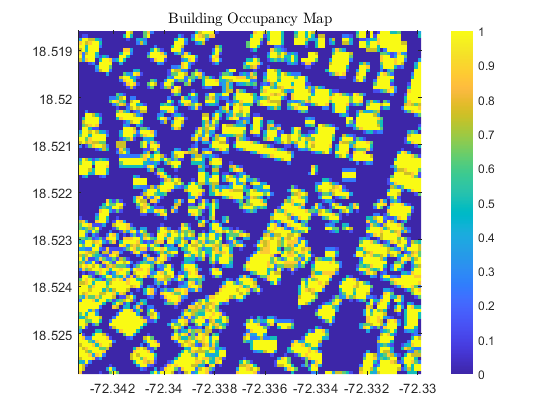
\includegraphics[width=\linewidth]{images/figures/m_bo.png}};
    \node (P0) at (8,4) {$p_{\text{bo}}$};
\end{scope}
\end{tikzpicture}
    \caption{Building Occupancy Grid}
    \label{fig:m_bo}
\end{figure}

% Resolutions
The environment and search map variables are shown in table \ref{tab:settings_general_cell}.
The environment map cell sizes were chosen as the fire model used in the simulation is based on a cell size of \SI{9}{\meter \square}.

\begin{table}[]
    \centering
    \caption{Environment and Search Map Variables}
    \label{tab:settings_general_cell}
    \begin{tabular}{r|l}
    \toprule
        Environment/Search Map Variable & Value \\
        \midrule
        $ l_{x_{e}} $ & \SI{3}{\meter}\\
        $ l_{y_{e}} $ & \SI{3}{\meter}\\ 
        $ l_{x_{s}} $ & \SI{15}{\meter}\\
        $ l_{y_{s}} $ & \SI{15}{\meter}\\
        $ n_{x_{e}} $ & 100\\
        $ n_{y_{e}} $ & 100\\
        $ n_{x_{s}} $ & 20\\
        $ n_{y_{s}} $ & 20\\
        \bottomrule
    \end{tabular}
\end{table}

% Wind map
The wind variables are shown in table \ref{tab:settings_general_wind}.
It is assumed that the wind direction and wind velocity are constant over the environment map, and therefore $\bm{M}_{v_{w}} =v_{w} \cdot \bm{1} $ and $\bm{M}_{\alpha_{w}} = \alpha_{w} \cdot \bm{1}$, where $\bm{1}$ is a matrix of ones of size $(n_{x_{e}}, n_{y_{e}})$).

\begin{table}[]
    \centering
    \caption{Wind Model Variables}
    \label{tab:settings_general_wind}
    \begin{tabular}{r|l}
    \toprule
        Wind Variable & Value \\
        \midrule
        $v_{w}$                     & \SI{1}{\meter \per \second}\\
        $\alpha_{w}$                & $\frac{\pi}{2}$ \\
        $\bm{M}_{v_{w}}$            & $v_{w} \cdot \bm{1}$\\
        $\bm{M}_{\alpha_{w}}$       & $\alpha_{w} \cdot \bm{1}$\\
        $r_{w}$                     & \SI{9}{\meter} \\
        $c_{\text{wm}_{1}}$         & 0.1 \\
        $c_{\text{wm}_{2}}$         & 0.1 \\
        $c_{\text{wm}_{d}}$         & 0.4 \\
        \bottomrule
    \end{tabular}
\end{table}

% Fire map

The fire variables are shown in table \ref{tab:settings_general_fire}.
The fire propagation distance is set to \SI{9}{\meter}, or three cells in each axis in the environment map.
The fire map is initialised according to the piecewise equation for all cells $ij$ in the environment map, where cells with building occupancy have a fire state of "flammable" if the building occupancy is not zero and "non flammable" otherwise, and one cell at location $(1,100)$ is set as "burning".
Figure \ref{fig:sim_fire_model} shows the spread of the fire through the disaster environment by the ignition time of each cell.

\begin{equation}
\label{eq:m_f_init_sim}
\begin{split}
    \bm{M}_{f}(i,j) = &
    \begin{cases} 
        0 & \bm{M}_{\text{bo}}(i,j) = 0 \\
        1 & \bm{M}_{\text{bo}}(i,j) > 0 \\
        3 & (i,j) \equiv (80:81,1:2) \\
    \end{cases} \\
    \forall i &= \{1, \ldots, n_{x_{e}}\}, j = \{1, \ldots, n_{y_{e}}\}
\end{split}
\end{equation}
% TO DO: update equation for current initialisation in matlab

\begin{table}[]
    \centering
    \caption{Fire Model Variables}
    \label{tab:settings_general_fire}
    \begin{tabular}{r|l}
    \toprule
        Fire Variable & Value \\
        \midrule
        $d_{\text{fp}} $            & \SI{9}{\meter} \\
        $c_{\text{fs}_{1}}$         & 0.2 \\
        $c_{\text{fs}_{2}}$         & 0.2  \\
        $t_{i}$                     & \SI{120}{\second} \\
        $t_{b}$                     & \SI{600}{\second} \\
        $\bm{M}_{f}(80,1)$          & 3\\
        \bottomrule
    \end{tabular}
\end{table}

\begin{figure}
    \centering
    \includegraphics{}
    \caption{Fire Spread over Disaster Environment}
    \label{fig:sim_fire_model}
\end{figure}

% Agents

The agent variables are shown in table \ref{tab:settings_general_agent}.
The the initial position of the agents is in the corner of the search map, with one agent in position $(1, 1)$ and one agent in position $(1, 2)$.
The initial target queue for the agents is their current location in position 1 and $\text{NaN}$ for all other positions in the queue.
The initial task of the agents is scanning, or $\bm{A}_{\text{task}} = (2, 2)$.

\begin{table}[]
    \centering
    \caption{Agent Variables}
    \label{tab:settings_general_agent}
    \begin{tabular}{r|l}
    \toprule
        Agent Variable & Value \\
        \midrule
        $n_{a}$                     & 2 \\
        $n_{q}$                     & 2 \\
        $t_{\text{scan}/m^{2}}$     & \SI{0.1}{\second} \\
        $\bm{A}_{\text{loc}}$       & \begin{pmatrix} 1 & 1 \\ 1 & 2 \end{pmatrix}\\
        $\bm{A}_{\text{target}}$    & \begin{pmatrix} 1 & 1 \\ 1 & 2 \\ \end{pmatrix} \begin{pmatrix} \text{NaN} & \text{NaN} \\ \text{NaN} & \text{NaN} \\ \end{pmatrix}\\
        $\bm{A}_{\text{task}}$      & \begin{pmatrix} 2 & 2 \end{pmatrix}\\
        $v_{\text{as}}$             & \SI{5}{\meter \per \second} \\
        \bottomrule
    \end{tabular}
\end{table}

% FIS

The \gls{fis} variables are shown in table \ref{tab:settings_general_fis}.
Figure \ref{fig:fis_mfs} shows a plot of the \gls{mf}s and figures \ref{fig:fis_output_surface_1, fig:fis_output_surface_2, fig:fis_output_surface_3} shows a plot of the initial output surface for each agent $a$.

\begin{table}[]
    \centering
    \caption{\gls{fis} Variables}
    \label{tab:settings_general_fis}
    \begin{tabular}{r|l}
    \toprule
        \gls{fis} Variable & Value \\
        \midrule
        $n_{i}$ & 3\\
        $n_{o}$ & 1\\
        \bottomrule
    \end{tabular}
\end{table}

\begin{figure}
    \centering
    \begin{tikzpicture}
\begin{scope}
    \node[anchor=south west,inner sep=0] (image) at (0,0) {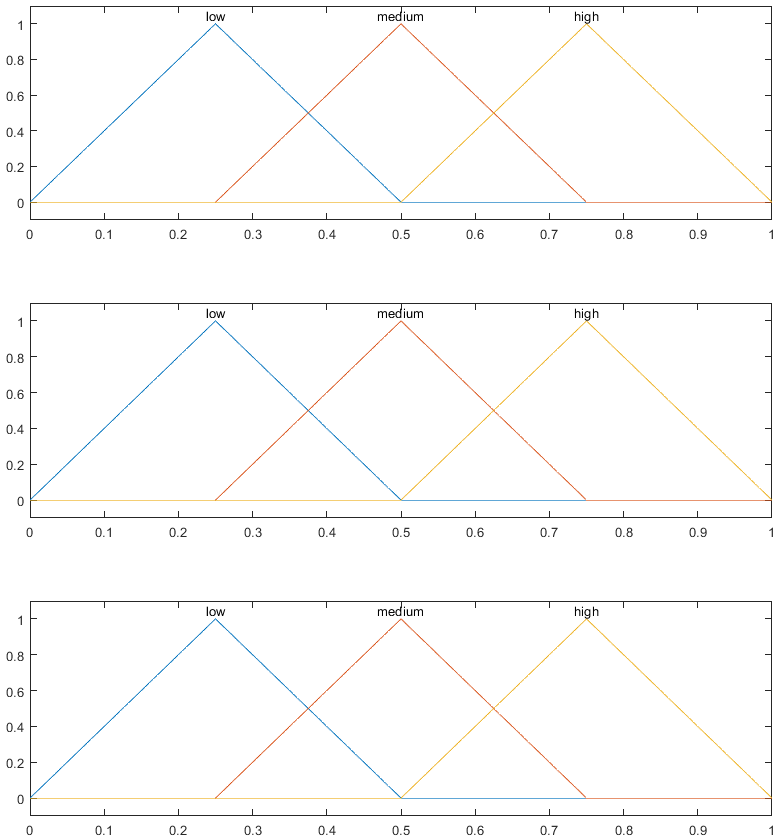
\includegraphics[width=\linewidth]{images/figures/fis.png}};
    \node (P0) at (5,6.5) {$\bar{t}_{\text{response}}$};
    \node (P1) at (5,3) {$p_{\text{prior}}$};
    \node (P2) at (5,-0.5) {$\bar{t}_{\text{dw}}$};
\end{scope}
\end{tikzpicture}
    \caption{\gls{mf}s for all inputs of agent $a$}
    \label{fig:fis_mfs}
\end{figure}

\begin{figure}
    \centering
    \begin{tikzpicture}
\begin{scope}
    \node[anchor=south west,inner sep=0] (i1) at (0,0) {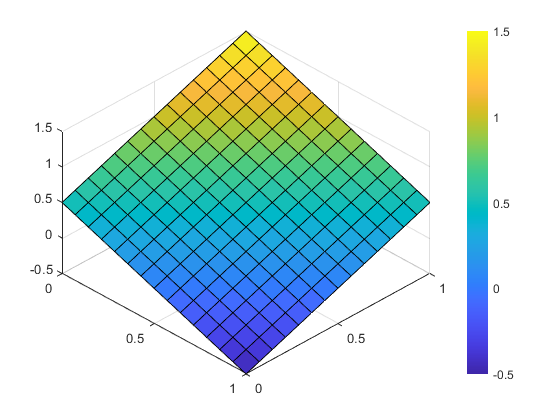
\includegraphics[width=\linewidth]{images/figures/fis_output_surf_t_dw_priority_clean.png}};
    \node (P0) at (0,3.5) {$p_{\text{att}}$};
    \node (P1) at (2,1) {$p_{\text{prior}}$};
    \node (P2) at (6,1) {$\bar{t}_{\text{dw}}$};
    \end{scope}
\end{tikzpicture}
    \caption{Initial output surface for agent $a$}
    \label{fig:fis_output_surface_1}
\end{figure}

\begin{figure}
    \centering
    \begin{tikzpicture}
\begin{scope}
    \node[anchor=south west,inner sep=0] (i1) at (0,0) {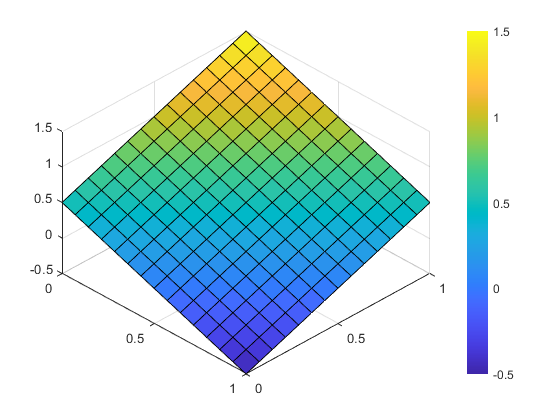
\includegraphics[width=\linewidth]{images/figures/fis_output_surf_t_response_priority_clean.png}};
    \node (P0) at (0,3.5) {$p_{\text{att}}$};
    \node (P1) at (2,1) {$\bar{t}_{\text{response}}$};
    \node (P2) at (6,1) {$p_{\text{prior}}$};
    \end{scope}
\end{tikzpicture}
    \caption{Initial output surface for agent $a$}
    \label{fig:fis_output_surface_2}
\end{figure}

\begin{figure}
    \centering
    \begin{tikzpicture}
\begin{scope}
    \node[anchor=south west,inner sep=0] (i1) at (0,0) {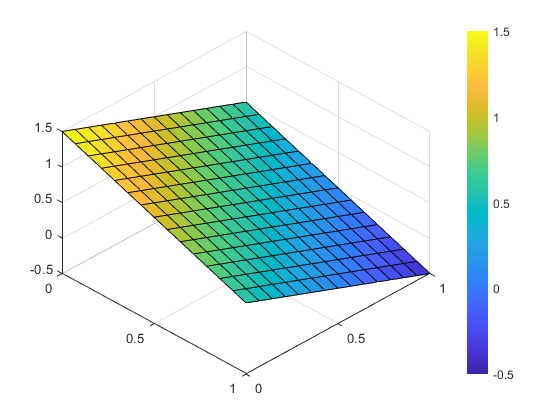
\includegraphics[width=\linewidth]{images/figures/fis_output_surf_t_response_t_dw_clean.png}};
    \node (P0) at (0,3.5) {$p_{\text{att}}$};
    \node (P1) at (2,1) {$\bar{t}_{\text{response}}$};
    \node (P2) at (6,1) {$\bar{t}_{\text{dw}}$};
    \end{scope}
\end{tikzpicture}
    \caption{Initial output surface for agent $a$}
    \label{fig:fis_output_surface_3}
\end{figure}

% MPC
The \gls{mpc} variables are shown in table \ref{tab:settings_general_mpc}.
The number of prediction time steps is set to 1 .
No minimum or maximum constraints for the output surface parameters are placed on the optimisation.

\begin{table}[]
    \centering
    \caption{\gls{mpc} Variables}
    \label{tab:settings_general_mpc}
    \begin{tabular}{r|l}
        \toprule
        \gls{mpc} Variable & Value \\
        \midrule
        $n_{p}$                     & 1\\
        $\bm{\theta}_{\text{min}}$  & $\text{NaN}$\\
        $\bm{\theta}_{\text{max}}$  & $\text{NaN}$\\
        \bottomrule
    \end{tabular}
\end{table}

% Constants

The constants are shown in table \ref{tab:settings_general_constants}.

\begin{table}[]
    \centering
    \caption{Constants}
    \label{tab:settings_general_constants}
    \begin{tabular}{r|l}
        \toprule
        Constants & Value \\
        \midrule
        $r_{\text{bo}}$ & 1 \\
        $r_{\text{es}}$ & 0.1 \\
        $r_{\text{fo}}$ & 0.5 \\
        \bottomrule
    \end{tabular}
\end{table}
% TO DO: check this is correct from matlab

\subsection{Functionality Tests Setup}
Functionality tests are tests that were run to analyse the design of the \gls{mpfc} controller by running specific simulations.
This section identifies the setup and goals of these tests.
% TO DO: run optimisation function test - rewrite sections

\subsubsection{Optimal Solver Test}
This functionality test was designed to determine the optimal solver to use for the \gls{mpc} solver block.
As mentioned, the optimisation problem is noncontinuous and multi-linear.
Therefore, the solvers selected for this test were the fminsearch, genetic algorithm, pattern search, and particle swarm algorithms.

The simulation was initialised using the default initialisation as discussed in section \ref{subsec:generalSimultionSetup}, and the \gls{mpc} module was activated with a solver constraint of the maximum time set to \SI{300}{\second}.
This constraint was selected as the real constraint on \gls{mpc} performance in a real application will be the maximum time that the solver can run for, as the \gls{mpc} must operate in real-time.
The objective to compare the solvers for was the best performance over the course of the simulation, or the lowest accumulative objective function.

\begin{figure}
    \centering
    \includegraphics{}
    \caption{Solver tests}
    \label{fig:plot_solver_test}
\end{figure}
% TO DO: include figure

The solver test results are shown in figure \ref{fig:plot_solver_test}.
Both the genetic algorithm and the particle swarm solvers greatly exceeded the maximum time constraint, as their initial evaluations took longer than the defined constraint, resulting in far worse time-performance than indicated.

\begin{figure}
    \centering
    \includegraphics{}
    \caption{Solver tests}
    \label{fig:plot_solver_test_init}
\end{figure}
% TO DO: include figure
 
The solver results for the first part of the simulation are shown in figure \ref{fig:plot_solver_test_init}.
As can be seen, the solver with the best rate of convergence was the pattern search solver, with an average performance \SI{?}{\percent} better then the genetic algorithm, \SI{?}{\percent} better then the particle swarm, and \SI{?}{\percent} better then the fmincon solvers.
Therefore, the pattern search solver was selected for the controller test simulations.

\subsubsection{\gls{fis} Sensitivity Test}

% TO DO: run simulation again?

This functionality test was designed to investigate the values of inputs and outputs of the \gls{fis}.
This information can be used to inform the design of the \gls{fis} controller, as the distribution of the values of inputs to the controller can be useful for the choice of \gls{mf} parameters.
For example, if the values for the priority input were mostly distributed lower in the range (closer to 0), then is might be preferable to have \gls{mf}s concentrated closer to the bottom of the range in order to provide greater control over the behaviour of the controller.

This test was run using the default initialisation described in section \ref{subsec:generalSimultionSetup} and with the \gls{mpc} controller deactivated.
All input and output values to the \gls{fis} over the course of the simulation were recorded, as shown in figure \ref{fig:SF02_scatter}.
Each input to the \gls{fis} is represented by one axis of the scatter plot, while the output of the \gls{fis} is represented by the colour scale applied to the data points.
It can be seen that the vast majority of data points are at the upper end of $\bar{t}_{\text{dw}}$ but are quite evenly distributed across $p_{\text{prior}}$ and $\bar{t}_{\text{response}}$.

\begin{figure*}
    \centering
    \begin{tikzpicture}
\begin{scope}
    \node[anchor=south west,inner sep=0] (image) at (0,0) {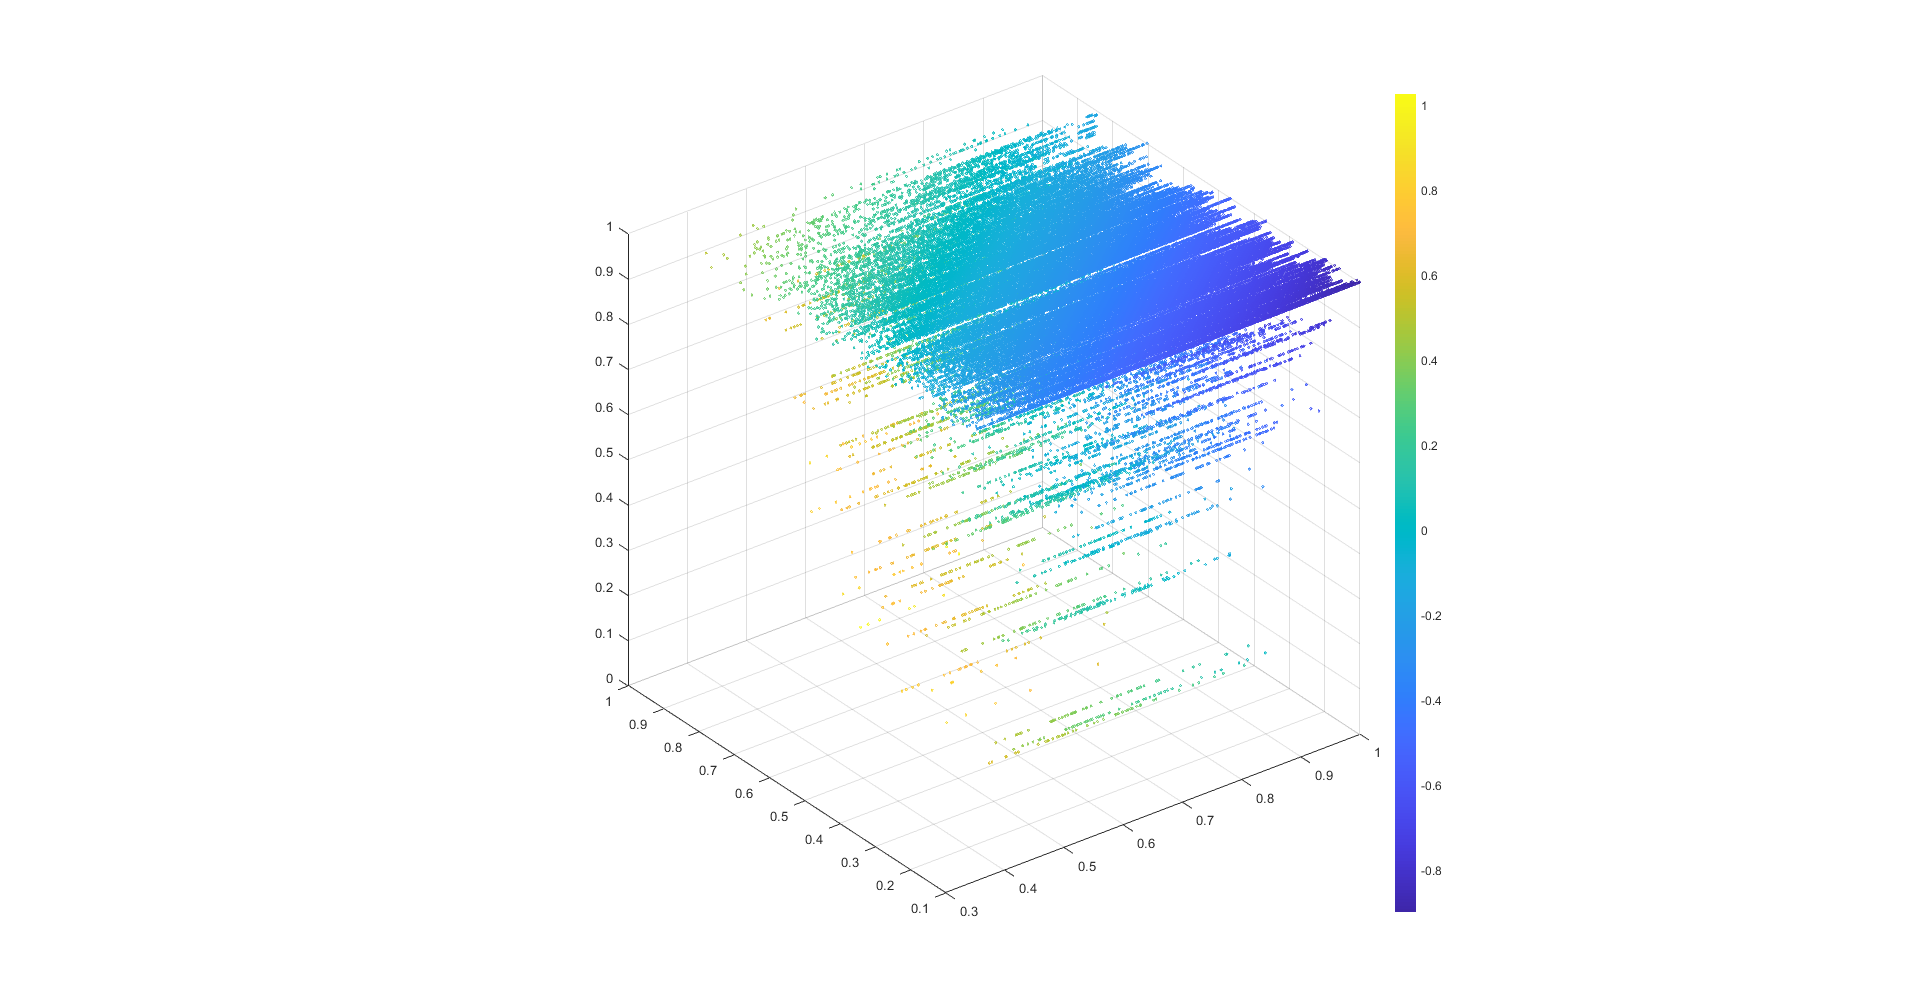
\includegraphics[width=\linewidth]{images/SF02/fis_sensitivity_clean.png}};
    \node (P0) at (14,5) {$p_{\text{att}}$};
    \node (P1) at (12,1) {$\bar{t}_{\text{response}}$};
    \node (P2) at (7,1) {$p_{\text{prior}}$};
    \node (P3) at (5,5) {$\bar{t}_{\text{dw}}$};
    \end{scope}
\end{tikzpicture}
    \caption{\gls{fis} Sensitivity Test Scatter}
    \label{fig:SF02_scatter}
\end{figure*}

% % Histograms
% \begin{figure*}
%     \centering
%     \begin{tikzpicture}
\begin{scope}
    \node[anchor=south west,inner sep=0] (image) at (0,0) {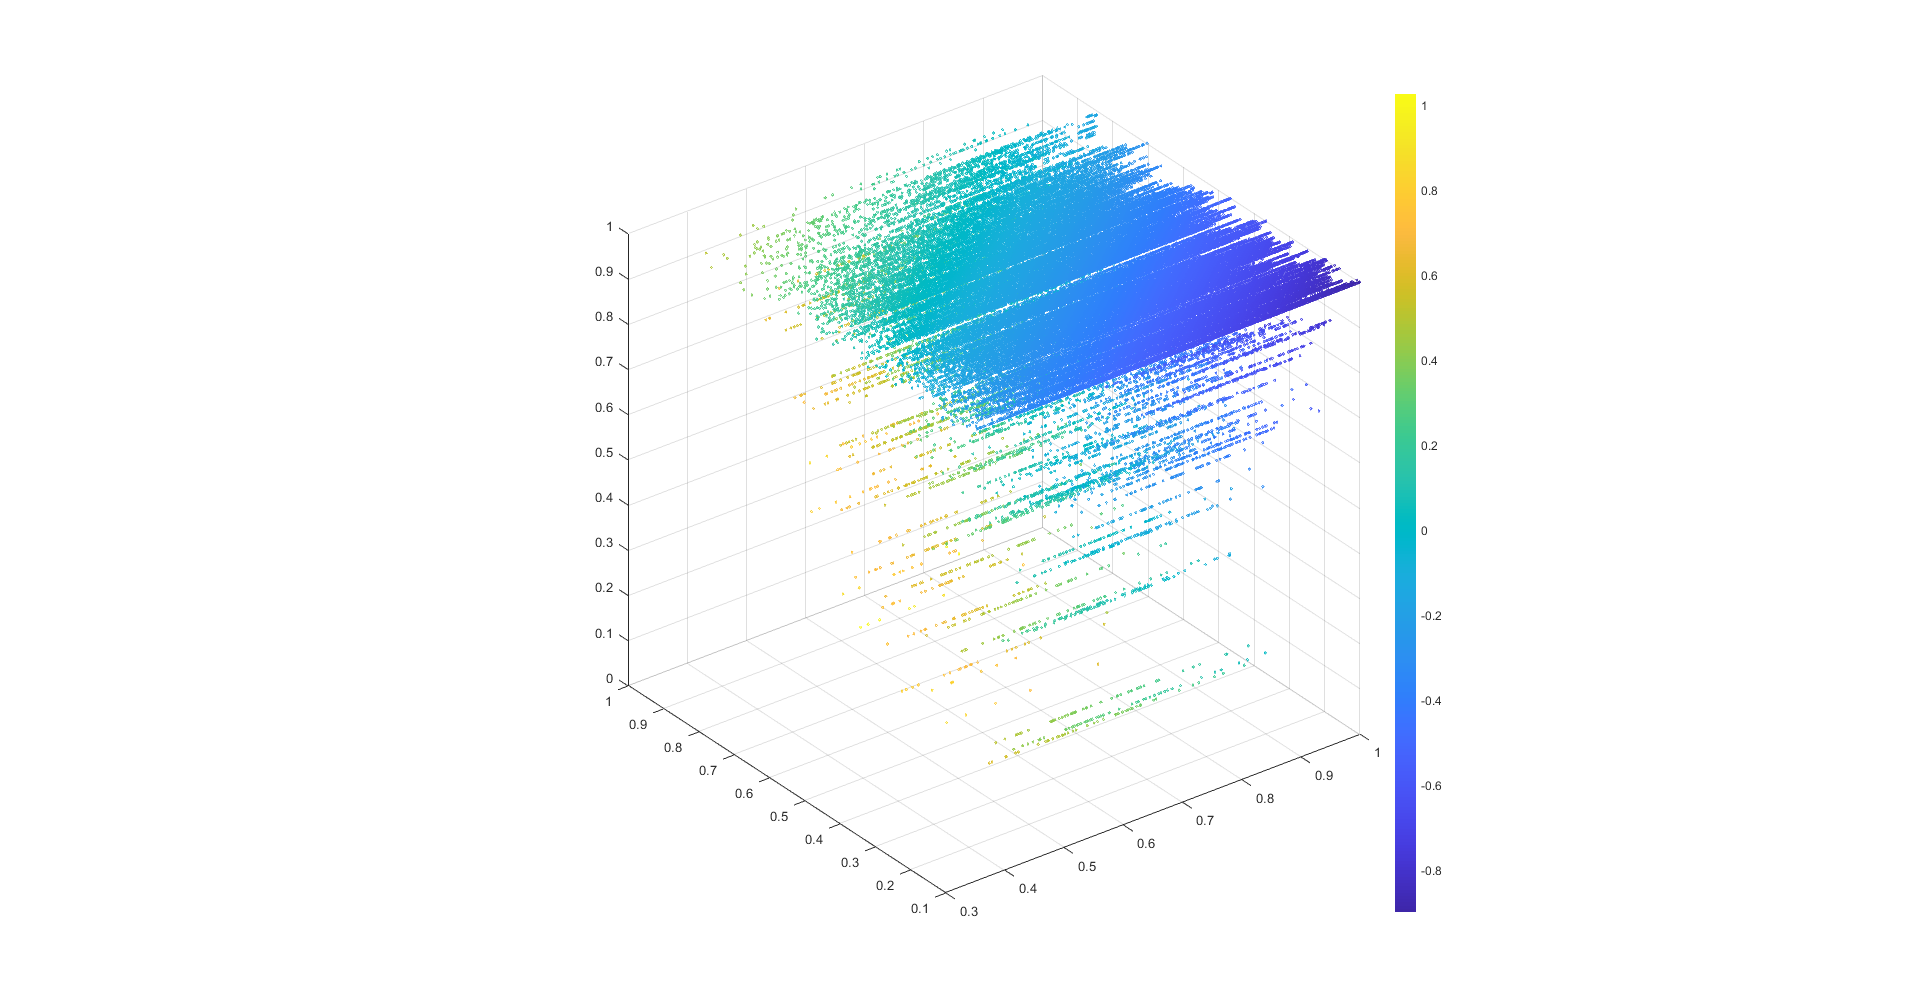
\includegraphics[width=\linewidth]{images/SF02/fis_sensitivity_clean.png}};
    \node (P0) at (14,5) {$p_{\text{att}}$};
    \node (P1) at (12,1) {$\bar{t}_{\text{response}}$};
    \node (P2) at (7,1) {$p_{\text{prior}}$};
    \node (P3) at (5,5) {$\bar{t}_{\text{dw}}$};
    \end{scope}
\end{tikzpicture}
%     \caption{\gls{fis} Sensitivity Test Scatter}
%     \label{fig:SF02_scatter}
% \end{figure*}
% TO DO: histograms of input values - plot in 1x3 multiplot

\subsubsection{Objective Function Sensitivity Test}

This functionality test was designed to investigate the sensitivity of the objective function to changes in the \gls{fis} output parameters.
This is important, as for the \gls{mpc} to be effective, the cost function should be dependent on the optimisation variables.
The \gls{mpc} module was disabled for this simulation, and instead the objective function sum was counted over the prediction horizon at each \gls{mpc} step for a 4x4 matrix of \gls{fis} output surface parameters for the first two \gls{mpc} steps in the simulation.
% TO DO: introduce ranges

\begin{table}[]
    \centering
    \caption{\gls{fis} Output Surface Parameters Values}
    \label{tab:SF03}
    \begin{tabular}{r|l}
        \toprule
        Parameter & Values \\
        \midrule
        $\bm{\theta}_{p_{\text{att}}}(1)$ & $(0, 0.6667, 1.3333, 2)$ \\
        $\bm{\theta}_{p_{\text{att}}}(2)$ & $(0, -0.6667, -1.3333, -2)$ \\
        $\bm{\theta}_{p_{\text{att}}}(3)$ & $(0, -0.6667, -1.3333, - 2)$ \\
        $\bm{\theta}_{p_{\text{att}}}(4)$ & $(0, 0.6667, 1.3333, 2)$ \\
        \bottomrule
    \end{tabular}
\end{table}

The objective function sensitivity test results are shown in figure \ref{fig:plot_mpc_sens_test}.
For all combinations of the range of output surface parameters, the objective function sum is evaluated over one prediction step.
As can be seen, changes to all four of the \gls{fis} output surface parameters result in different evaluations of the objective function sum, indicating that the behaviour of the agents is dependent upon all of the output surface parameters, and hence inputs.
It can be seen that for some combinations of output surface parameters, the objective function sum remains the same, indicating that the behaviour of the agents is the same.
As this test is only run for one prediction time step, the this combination of output surface parameters may result in different agent behaviour for other instances of the simulation, but not for the current instance of the simulation.

\begin{figure}
    \centering
    \includegraphics{}
    \caption{\gls{mpc} Sensitivity Test}
    \label{fig:plot_mpc_sens_test}
\end{figure}

\subsection{Controller Simulations Setup}

The controller simulation sets are sets of simulations designed to analyse the performance of the \gls{mpfc} controller.
In each simulation set, the initialisation and models used are exactly the same except for the \gls{mpc} model.
The first simulation in each controller simulation set has the \gls{mpc} disabled to provide a baseline for the performance of the path-planning controller.
The other simulations in the simulation set have the \gls{mpc} controller active with different constraints on the maximum number of function evaluations of the solver, as shown in table \ref{tab:CSS_simulations}.

\begin{table}[]
    \centering
    \caption{Simulations in each controller simulation set}
    \label{tab:CSS_simulations}
    \begin{tabular}{r|ll}
    \toprule
        Simulation # & \gls{mpc} Active & $n_{\text{fe}_{\text{max}}}$ \\
        \midrule
        1 & False & N/A \\
        2 & True & 10\\
        3 & True & 40\\
        4 & True & 100\\
        \bottomrule
    \end{tabular}
\end{table}

\subsubsection{Simulation 1 - Default}  \label{subsubsec:SS01}

This simulation test was run with all default values defined in section \ref{subsec:generalSimultionSetup}.
This was selected as the minimum viable system and controller setup for analysing the performance of the \gls{mpfc} controller.
As mentioned, the \gls{fis} has one output surface, resulting in a completely linear output from the \gls{fis}.
This results in the rule base having no effect on the performance of the \gls{fis}, as all rules point to the same output surface.
In order to benefit from the full advantages of the \gls{fis}, multiple output surfaces would be desired to benefit from the additional complexity introduced by the rule base, however, this greatly increases the number of optimisation variables that the \gls{mpc} must deal with, so initial simulations sets were conducted with one output surface, resulting in a total number of optimisation variables, $n_{\text{optvar}} = 4 n_{a} n_{p} n_{\mu_{\text{out}}} = 8$.

\subsubsection{Simulation 2 - Three Agents} \label{subsubsec:SS02}

This simulation test was initialised with an additional agent, as shown in table \ref{tab:settings_SS02}.
The agent location was initialised in the cell adjacent to the other agents with the task to scan its starting location cell, resulting in a total number of optimisation variables, $n_{\text{optvar}} = 4 n_{a} n_{p} n_{\mu_{\text{out}}} = 12$.

\begin{table}[]
    \centering
    \caption{Agent Variables}
    \label{tab:settings_SS02}
    \begin{tabular}{r|l}
    \toprule
        Variable & Value \\
        \midrule
        $n_{a}$                     & 3 \\
        $\bm{A}_{\text{loc}}$       & \begin{pmatrix} 1 & 1 \\ 1 & 2 \\ 1 & 3 \end{pmatrix}\\
        $\bm{A}_{\text{target}}$    & \begin{pmatrix} 1 & 1 \\ 1 & 2 \\ 1 & 3 \end{pmatrix} \begin{pmatrix} \text{NaN} & \text{NaN} \\ \text{NaN} & \text{NaN} \\ \text{NaN} & \text{NaN} \end{pmatrix}\\
        $\bm{A}_{\text{task}}$      & \begin{pmatrix} 1 & 1 & 1 \end{pmatrix}\\
        \bottomrule
    \end{tabular}
\end{table}

\subsubsection{Simulation 3 - Two Prediction Time-steps} \label{subsubsec:SS03}

This simulation test was initialised with an additional prediction time step, as shown in table \ref{tab:settings_SS03}, resulting in a total number of optimisation variables, $n_{\text{optvar}} = 4 n_{a} n_{p} n_{\mu_{\text{out}}} = 16$ for each optimisation.

\begin{table}[]
    \centering
    \caption{Variables}
    \label{tab:settings_SS03}
    \begin{tabular}{r|l}
        \toprule
        Variable & Value \\
        \midrule
        $n_{p}$ & 2\\
        \bottomrule
    \end{tabular}
\end{table}

\subsubsection{Simulation 4 - Three Queue Length} \label{subsubsec:SS04}

This simulation test was initialised with an additional prediction time step, as shown in table \ref{tab:settings_SS04}.

\begin{table}[]
    \centering
    \caption{Variables}
    \label{tab:settings_SS04}
    \begin{tabular}{r|l}
        \toprule
        Variable & Value \\
        \midrule
        $n_{q}$ & 3 \\
        \bottomrule
    \end{tabular}
\end{table}

\subsubsection{Simulation 5 - Two Output Surfaces} \label{subsubsec:SS05}

For this simulation, the number of output surfaces is increased to $n_{\mu_{\text{out}}} = 2$, resulting in a total number of optimisation variables, $n_{\text{optvar}} = 4 n_{a} n_{p} n_{\mu_{\text{out}}} = 16$ for each optimisation.
The additional output surface, $\mu_{p_{\text{att}_{a_{2}}}}$, was initialised using the same values as the previous output surface, as shown in table \ref{tab:settings_SS05}.
The rule base is given by table \ref{tab:fis_rulebase}.
The two output surfaces are chosen to be for high-attraction outputs and low-attraction outputs respectively.
Rules were hand-designed accordingly to distribute the input membership functions to the appropriate output surface.

% FIS parameters
\begin{table}
    \centering
    \caption{Initial output parameters for \gls{fis} of agent $a$}
    \label{tab:settings_SS05}
    \begin{tabular}{r|cccc}
        \toprule
        Output & $\bm{\theta}_{\mu_{p_{\text{att}_{a}}}}(1)$ & $\bm{\theta}_{\mu_{p_{\text{att}_{a}}}}(2)$ & $\bm{\theta}_{\mu_{p_{\text{att}_{a}}}}(3)$ & $\bm{\theta}_{\mu_{p_{\text{att}_{a}}}}(4)$ \\
        \midrule
         $\mu_{p_{\text{att}_{a_{1}}}}$ & 1 & -1 & -1 & 1 \\
         $\mu_{p_{\text{att}_{a_{2}}}}$ & 1 & -1 & -1 & 1 \\
        \bottomrule
    \end{tabular}
\end{table}

% FIS Rule Base
\begin{table}[]
    \centering
    \caption{Rule base for \gls{fis} for an agent $a$}
    \label{tab:fis_rulebase}
    \begin{tabular}{cccc}
    \toprule
        $\mu_{\bar{t}_{\text{response}_{a}}}$ & $\mu_{p_{\text{prior}_{a}}}$ & $\mu_{\bar{t}_{\text{dw}_{a}}}$ & $\mu_{p_{\text{att}_{a}}}$ \\    
    \midrule
        1 & 1 & 1 & 2 \\
        1 & 1 & 2 & 1 \\
        1 & 1 & 3 & 1 \\
        1 & 2 & 1 & 2 \\
        1 & 2 & 2 & 2 \\
        1 & 2 & 3 & 2 \\
        1 & 3 & 1 & 2 \\
        1 & 3 & 2 & 2 \\
        1 & 3 & 3 & 2 \\
        2 & 1 & 1 & 1 \\
        2 & 1 & 2 & 1 \\
        2 & 1 & 3 & 1 \\
        2 & 2 & 1 & 2 \\
        2 & 2 & 2 & 2 \\
        2 & 2 & 3 & 1 \\
        2 & 3 & 1 & 2 \\
        2 & 3 & 2 & 2 \\
        2 & 3 & 3 & 2 \\
        3 & 1 & 1 & 1 \\
        3 & 1 & 2 & 1 \\
        3 & 1 & 3 & 1 \\
        3 & 2 & 1 & 1 \\
        3 & 2 & 2 & 1 \\
        3 & 2 & 3 & 2 \\
        3 & 3 & 1 & 2 \\
        3 & 3 & 2 & 2 \\
        3 & 3 & 3 & 1 \\
        \bottomrule
    \end{tabular}
\end{table}

% Initial FIS parameters

\subsubsection{Simulation 6 - Two Output Surfaces and Two Prediction Steps} \label{subsubsec:SS06}
For this simulation, the number of prediction steps is increased to $n_{p} = 2$, resulting in a total number of optimisation variables, $n_{\text{optvar}} = 4 n_{a} n_{p} n_{\mu_{\text{out}}} = 32$ for each optimisation.


\begin{table}[]
    \centering
    \caption{Variables}
    \label{tab:settings_SS06}
    \begin{tabular}{r|l}
        \toprule
        Variable & Value \\
        \midrule
        $n_{p}$ & 2 \\
        \bottomrule
    \end{tabular}
\end{table}

\subsubsection{Simulation 7 - Two Output Surfaces and Three Prediction Steps} \label{subsubsec:SS07}
For this simulation, the number of prediction steps is increased to $n_{p} = 3$, resulting in a total number of optimisation variables, $n_{\text{optvar}} = 4 n_{a} n_{p} n_{\mu_{\text{out}}} = 48$ for each optimisation.

\begin{table}[]
    \centering
    \caption{Variables}
    \label{tab:settings_SS07}
    \begin{tabular}{r|l}
        \toprule
        Variable & Value \\
        \midrule
        $n_{p}$ & 3 \\
        \bottomrule
    \end{tabular}
\end{table}

\subsubsection{Simulation 8 - Two Output Surfaces and Three Prediction Steps with Extended Prediction Time Step} \label{subsubsec:SS08}
For this simulation, the size of the prediction steps is increased to $\Delta k_{\text{mpc}} = 480$, resulting in a prediction step time of $\Delta t_{\text{mpc}} =  \Delta k_{\text{mpc}} \Delta t_{k}$.

\begin{table}[]
    \centering
    \caption{Variables}
    \label{tab:settings_SS08}
    \begin{tabular}{r|l}
        \toprule
        Variable & Value \\
        \midrule
        $n_{p}$ & 3 \\
        \bottomrule
    \end{tabular}
\end{table}

\section{Results} \label{sec:results} 

 \subsection{Simulation 1 - Default}  \label{subsec:results_SS01}

% obj function by time
\begin{figure}[h]
    \centering
    \begin{tikzpicture}
\begin{scope}
    \node[anchor=south west,inner sep=0] (image) at (0,0) {\includegraphics[width=\linewidth]{images/SS01/obj_hist.jpg}};
    \node (P0) at (0,3.5) {$J$};
    \node (P0) at (5,0) {Time (\si{\second})};
\end{scope}
\end{tikzpicture}
    \caption{Objective function over time for simulation 1}
    \label{fig:SS01_obj_hist}
\end{figure}

% % relative objective function
% \begin{figure}[h]
%     \centering
%     \begin{tikzpicture}
\begin{scope}
    \node[anchor=south west,inner sep=0] (image) at (0,0) {\includegraphics[width=\linewidth]{images/SS01/obj_hist_relative.jpg}};
    \node (P0) at (0,3.5) {$\frac{J_{\text{sim}}}{J_{1}}$};
    \node (P0) at (5,0) {Time (\si{\second})};
\end{scope}
\end{tikzpicture}
%     \caption{Relative performance for simulation 1}
%     \label{fig:SS01_obj_hist_rel}
% \end{figure}

% obj function sum
\begin{figure}[h]
    \centering
    \begin{tikzpicture}
\begin{scope}
    \node[anchor=south west,inner sep=0] (image) at (0,0) {\includegraphics[width=\linewidth]{images/SS01/s_obj_hist.jpg}};
    \node (P0) at (0,3.5) {$\sum_{k_{i}=0}^{k} J$};
    \node (P0) at (5,0) {Time (\si{\second})};
\end{scope}
\end{tikzpicture}
    \caption{Objective function sum over time for simulation 1}
    \label{fig:SS01_s_obj_hist}
\end{figure}

% relative objective function sum
\begin{figure}[h]
    \centering
    \begin{tikzpicture}
\begin{scope}
    \node[anchor=south west,inner sep=0] (image) at (0,0) {\includegraphics[width=\linewidth]{images/SS01/s_obj_hist_relative.jpg}};
    \node (P0) at (-0.5,3.5) {$\frac{\sum_{k_{i}=0}^{k} J_{\text{sim}}}{\sum_{k_{i}=0}^{k} J_{1}}$};
    \node (P0) at (5,0) {Time (\si{\second})};
\end{scope}
\end{tikzpicture}
    \caption{Relative performance for simulation 1}
    \label{fig:SS01_s_obj_rel}
\end{figure}

% % FIS output surface parameters
% \begin{figure}[h]
%     \centering
%     \includegraphics{}
%     \caption{FIS output surface parameters for simulation 1}
%     \label{fig:SS01_fis_params}
% \end{figure} 

% The objective function over time is shown in figure \ref{fig:SS01_obj_hist}, the objective function sum over time in figure \ref{fig:SS01_s_obj_hist}, the relative performance in figure \ref{fig:SS01_s_obj_rel}, and the \gls{fis} parameters in figure \ref{fig:SS01_fis_params}.
% It can be seen that when the \gls{mpc} is run with very few function evaluations, the performance can be worse than the pre-tuned \gls{fis}.
All of the simulations with the \gls{mpc} active performed better than the control simulation with the \gls{mpc} deactivated.
The relative performance of the simulations with respect to the control simulation is shown in figure \ref{fig:SS01_s_obj_rel}, where the objective function sum history for each simulation is divided by the control simulation.
The controller with the best performance is for $n_{\text{fe}_{\text{max}}} = 10$ with about \SI{4}{\percent} improvement, followed by $n_{\text{fe}_{\text{max}}} = 40$ with about \SI{3}{\percent} improvement and $n_{\text{fe}_{\text{max}}} = 100$ with about \SI{2}{\percent} improvement.

These results were not expected, as it is hypothesised that with more function evaluations, the \gls{mpc} will perform better.
Several possible contributing factors to this were identified.
Firstly, the prediction horizon may be too short to predict the long-term effects of optimising \gls{fis} parameters in the short term.
For instance, the \gls{mpc} with 100 function evaluations may have optimised performance slightly better at the start of the simulation, but ended up in a position that resulted in a large decrease in performance shortly after.

\subsection{Simulation 2 - Three Agents} \label{subsec:results_SS02}

% obj function by time
\begin{figure}[h]
    \centering
    \begin{tikzpicture}
\begin{scope}
    \node[anchor=south west,inner sep=0] (image) at (0,0) {\includegraphics[width=\linewidth]{images/SS02/obj_hist.jpg}};
    \node (P0) at (0,3.5) {$J$};
    \node (P0) at (5,0) {Time (\si{\second})};
\end{scope}
\end{tikzpicture}
    \caption{Objective function over time for simulation 2}
    \label{fig:SS02_obj_hist}
\end{figure} 

% % relative objective function
% \begin{figure}[h]
%     \centering
%     \begin{tikzpicture}
\begin{scope}
    \node[anchor=south west,inner sep=0] (image) at (0,0) {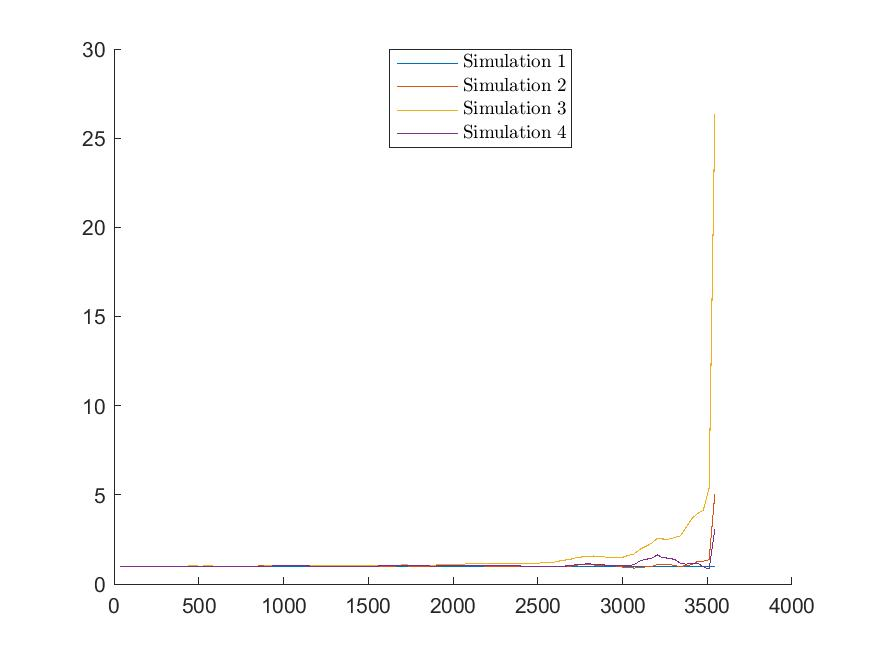
\includegraphics[width=\linewidth]{images/SS02/obj_hist_relative.jpg}};
    \node (P0) at (0,3.5) {$\frac{J_{\text{sim}}}{J_{1}}$};
    \node (P0) at (5,0) {Time (\si{\second})};
\end{scope}
\end{tikzpicture}
%     \caption{Relative performance for simulation 2}
%     \label{fig:SS02_obj_hist_rel}
% \end{figure}

% obj function sum
\begin{figure}[h]
    \centering
    \begin{tikzpicture}
\begin{scope}
    \node[anchor=south west,inner sep=0] (image) at (0,0) {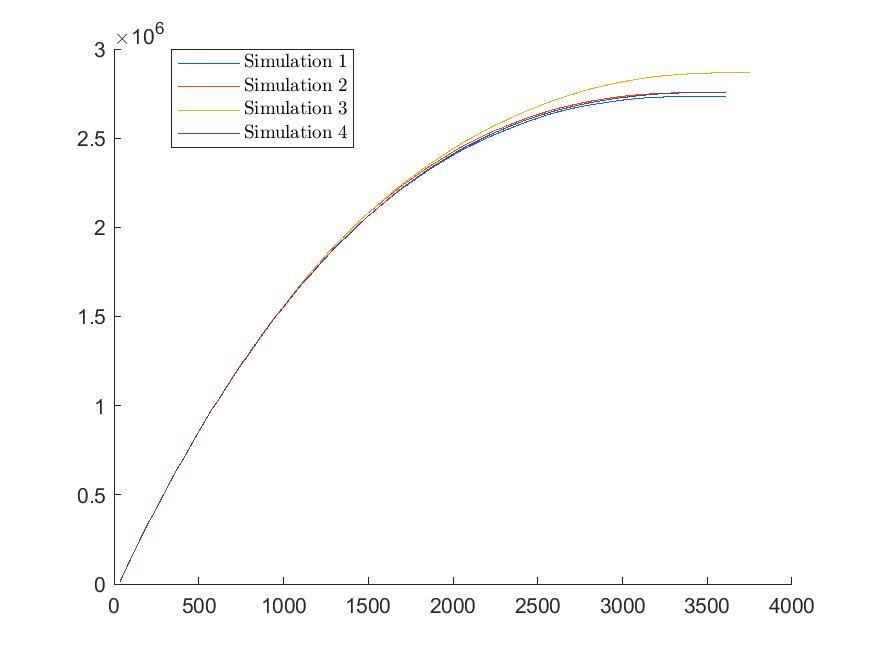
\includegraphics[width=\linewidth]{images/SS02/s_obj_hist.jpg}};
    \node (P0) at (0,3.5) {$\sum_{k_{i}=0}^{k} J$};
    \node (P0) at (5,0) {Time (\si{\second})};
\end{scope}
\end{tikzpicture}
    \caption{Objective function sum over time for simulation 2}
    \label{fig:SS02_s_obj_hist}
\end{figure}

% obj function sum
\begin{figure}[h]
    \centering
    \begin{tikzpicture}
\begin{scope}
    \node[anchor=south west,inner sep=0] (image) at (0,0) {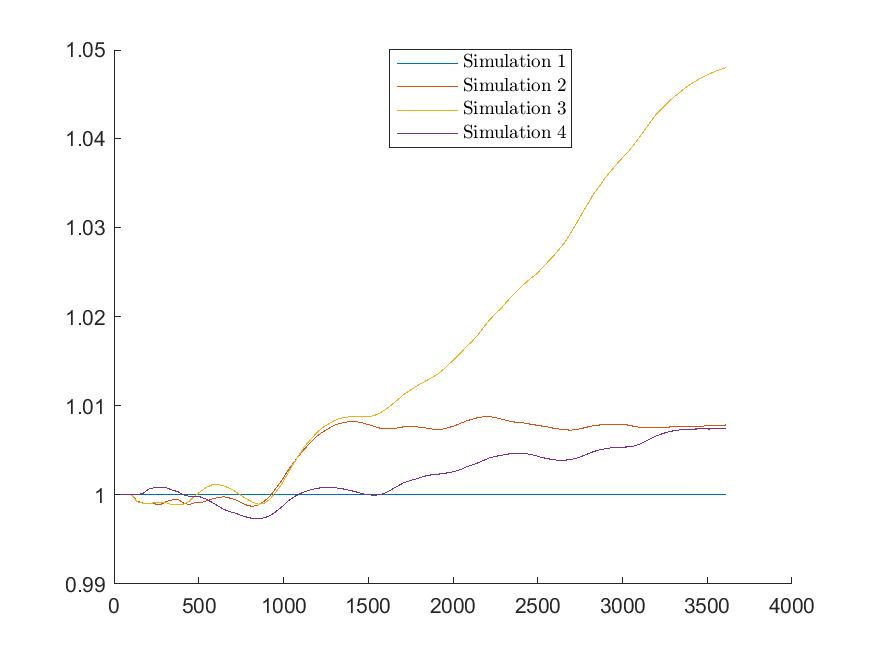
\includegraphics[width=\linewidth]{images/SS02/s_obj_hist_relative.jpg}};
    \node (P0) at (-0.5,3.5) {$\frac{\sum_{k_{i}=0}^{k} J_{\text{sim}}}{\sum_{k_{i}=0}^{k} J_{1}}$};
    \node (P0) at (5,0) {Time (\si{\second})};
\end{scope}
\end{tikzpicture}
    \caption{Relative performance for simulation 2}
    \label{fig:SS02_s_obj_rel}
\end{figure}

% % FIS output surface parameters
% \begin{figure}
%     \centering
%     \includegraphics{}
%     \caption{FIS output surface parameters for simulation 2}
%     \label{fig:SS01_fis_params}
% \end{figure}

In this simulation set, all of the simulations with the \gls{mpc} active performed worse than the control simulation.
The relative performance of the simulations with respect to the control simulation is shown in figure \ref{fig:SS01_s_obj_rel}.
It can be seen that the simulations with $n_{\text{fe}_{\text{max}}} = 10$ and $n_{\text{fe}_{\text{max}}} = 100$ performed about \SI{1}{\percent} worse than the control simulation and the simulation with $n_{\text{fe}_{\text{max}}} = 40$ had about \SI{4}{\percent} worse performance.

These results were not expected, as it is expected that with the \gls{mpc} module active, the \gls{sar} system should have improved performance.
All simulations with the \gls{mpc} active demonstrated improved performance in the short term - up to around \SI{1000}{\second} into the simulation.
The \gls{mpc} may have optimised performance over the prediction horizon for the first prediction step, but managed to put the agents in a position which degraded their performance further in the future.
This seems unlikely, however, as the prediction horizon was set to \SI{1440}{\second}, at which time all simulations with the \gls{mpc} active had worse performance than the control simulation.
Another possible factor is that with the increased number of optimisation variables, the number of function evaluations was insufficient to find an optimal solution to the optimisation problem.

\subsection{Simulation 3 - Two Prediction Time-steps} \label{subsec:results_SS03}

% obj function by time
\begin{figure}[h]
    \centering
    \begin{tikzpicture}
\begin{scope}
    \node[anchor=south west,inner sep=0] (image) at (0,0) {\includegraphics[width=\linewidth]{images/SS03/obj_hist.jpg}};
    \node (P0) at (0,3.5) {$J$};
    \node (P0) at (5,0) {Time (\si{\second})};
\end{scope}
\end{tikzpicture}
    \caption{Objective function over time for simulation 3}
    \label{fig:SS03_obj_hist}
\end{figure} 

% % relative objective function
% \begin{figure}[h]
%     \centering
%     \begin{tikzpicture}
\begin{scope}
    \node[anchor=south west,inner sep=0] (image) at (0,0) {\includegraphics[width=\linewidth]{images/SS03/obj_hist_relative.jpg}};
    \node (P0) at (0,3.5) {$\frac{J_{\text{sim}}}{J_{1}}$};
    \node (P0) at (5,0) {Time (\si{\second})};
\end{scope}
\end{tikzpicture}
%     \caption{Relative performance for simulation 3}
%     \label{fig:SS03_obj_hist_rel}
% \end{figure}

% obj function sum
\begin{figure}[h]
    \centering
    \begin{tikzpicture}
\begin{scope}
    \node[anchor=south west,inner sep=0] (image) at (0,0) {\includegraphics[width=\linewidth]{images/SS03/s_obj_hist.jpg}};
    \node (P0) at (0,3.5) {$\sum_{k_{i}=0}^{k} J$};
    \node (P0) at (5,0) {Time (\si{\second})};
\end{scope}
\end{tikzpicture}
    \caption{Objective function sum over time for simulation 3}
    \label{fig:SS03_s_obj_hist}
\end{figure}

% obj function sum
\begin{figure}[h]
    \centering
    \begin{tikzpicture}
\begin{scope}
    \node[anchor=south west,inner sep=0] (image) at (0,0) {\includegraphics[width=\linewidth]{images/SS03/s_obj_hist_relative.jpg}};
    \node (P0) at (-0.5,3.5) {$\frac{\sum_{k_{i}=0}^{k} J_{\text{sim}}}{\sum_{k_{i}=0}^{k} J_{1}}$};
    \node (P0) at (5,0) {Time (\si{\second})};
\end{scope}
\end{tikzpicture}
    \caption{Relative performance for simulation 3}
    \label{fig:SS03_s_obj_rel}
\end{figure}

% % FIS output surface parameters
% \begin{figure}
%     \centering
%     \includegraphics{}
%     \caption{FIS output surface parameters for simulation 3}
%     \label{fig:SS03_fis_params}
% \end{figure}

In this simulation set, the results were identical to simulation 1 (section \ref{subsec:results_SS01}).
This indicates that the solver was not able to find a more optimal set of parameters over the longer prediction horizon than it found for simulation \ref{subsec:results_SS01}.
This may imply that the number of function evaluations was not large enough to calculate an optimal solution over two prediction timesteps, and the solver reverted to using the initial optimal result it found for the first prediction step, or that the actions of the agents during the first prediction step may far outweigh the actions of the agents during subsequent prediction steps.
This may be possible, as the objective function is highest during the start of the simulation and consistently decreases.

% This is logical, as the agents always recalculate their next target before they commit to it.
% This component of the controller, however, would be useful in situations where the agents cannot always reliably communicate with other agents in the system in order to plan their next tasks, as they would have a list of the cells which other agents intend to scan in the future.

\subsection{Simulation 4 - Three Queue Length} \label{subsec:results_SS04}

% obj function by time
\begin{figure}[h]
    \centering
    \begin{tikzpicture}
\begin{scope}
    \node[anchor=south west,inner sep=0] (image) at (0,0) {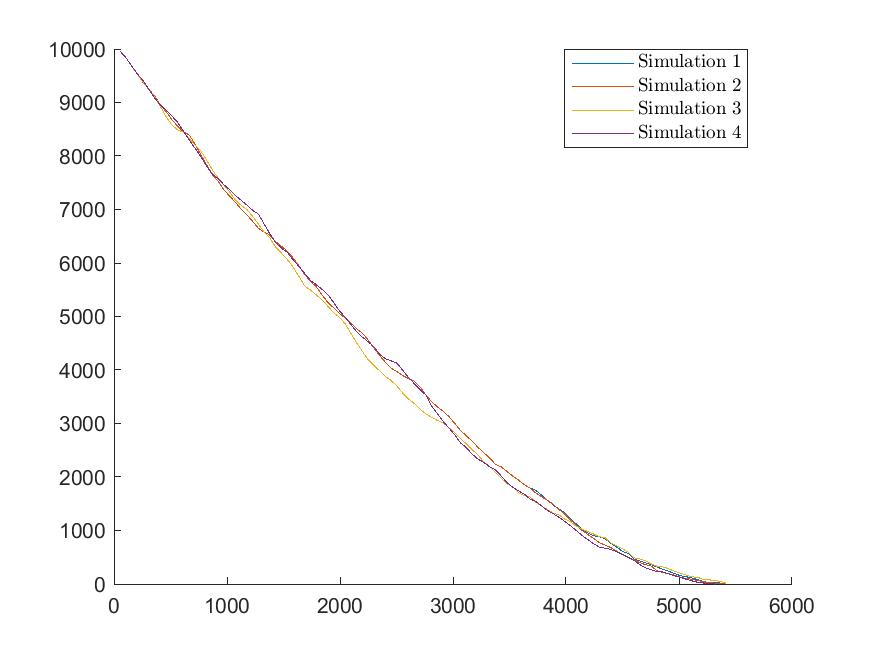
\includegraphics[width=\linewidth]{images/SS04/obj_hist.jpg}};
    \node (P0) at (0,3.5) {$J$};
    \node (P0) at (5,0) {Time (\si{\second})};
\end{scope}
\end{tikzpicture}
    \caption{Objective function over time for simulation 4}
    \label{fig:SS04_obj_hist}
\end{figure} 

% % relative objective function
% \begin{figure}[h]
%     \centering
%     \begin{tikzpicture}
\begin{scope}
    \node[anchor=south west,inner sep=0] (image) at (0,0) {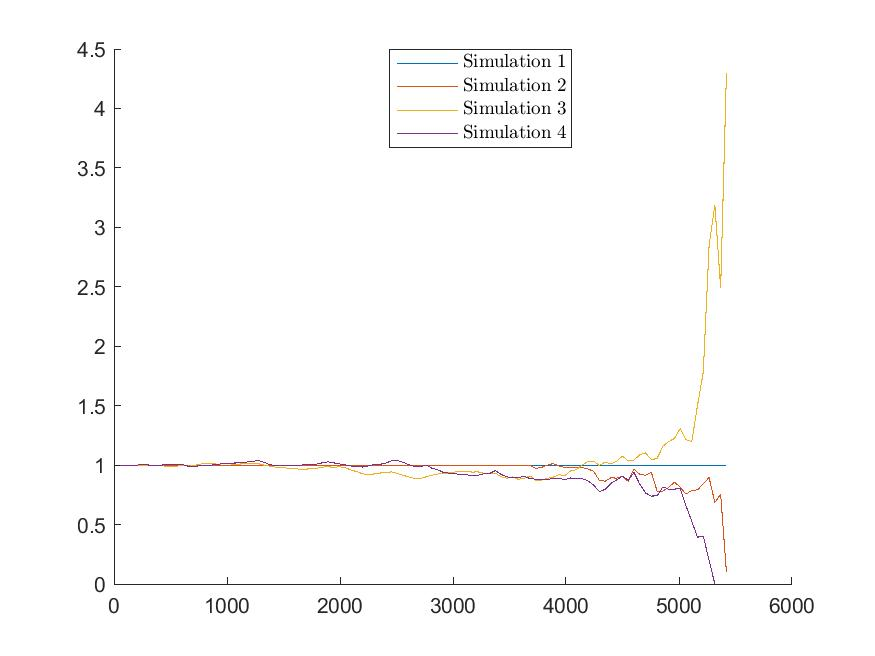
\includegraphics[width=\linewidth]{images/SS04/obj_hist_relative.jpg}};
    \node (P0) at (0,3.5) {$\frac{J_{\text{sim}}}{J_{1}}$};
    \node (P0) at (5,0) {Time (\si{\second})};
\end{scope}
\end{tikzpicture}
%     \caption{Relative performance for simulation 4}
%     \label{fig:SS04_obj_hist_rel}
% \end{figure}

% obj function sum
\begin{figure}[h]
    \centering
    \begin{tikzpicture}
\begin{scope}
    \node[anchor=south west,inner sep=0] (image) at (0,0) {\includegraphics[width=\linewidth]{images/SS04/s_obj_hist.jpg}};
    \node (P0) at (0,3.5) {$\sum_{k_{i}=0}^{k} J$};
    \node (P0) at (5,0) {Time (\si{\second})};
\end{scope}
\end{tikzpicture}
    \caption{Objective function sum over time for simulation 4}
    \label{fig:SS04_s_obj_hist}
\end{figure}

% relative objective function sum
\begin{figure}[h]
    \centering
    \begin{tikzpicture}
\begin{scope}
    \node[anchor=south west,inner sep=0] (image) at (0,0) {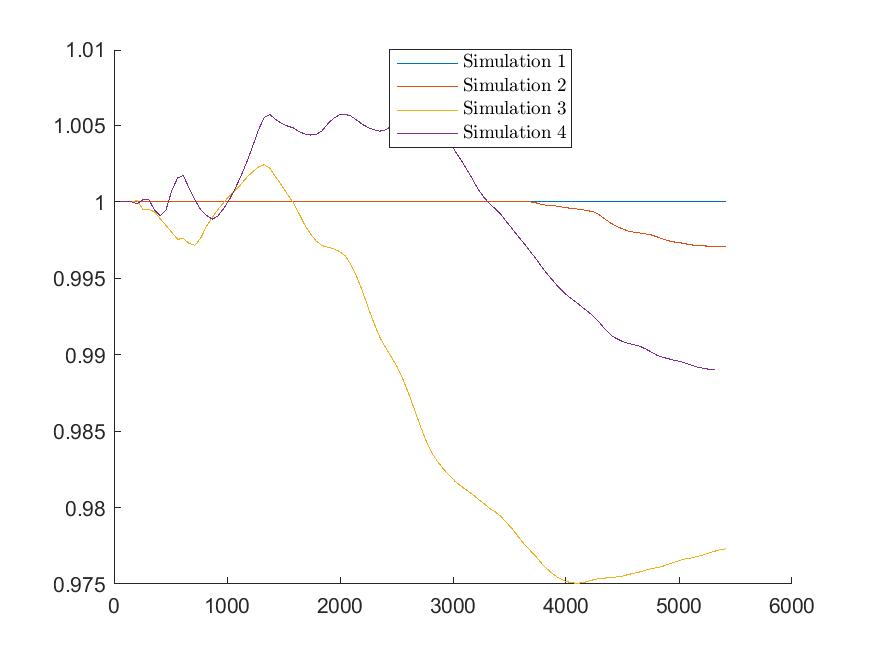
\includegraphics[width=\linewidth]{images/SS04/s_obj_hist_relative.jpg}};
    \node (P0) at (-0.5,3.5) {$\frac{\sum_{k_{i}=0}^{k} J_{\text{sim}}}{\sum_{k_{i}=0}^{k} J_{1}}$};
    \node (P0) at (5,0) {Time (\si{\second})};
\end{scope}
\end{tikzpicture}
    \caption{Relative performance for simulation 4}
    \label{fig:SS04_s_obj_rel}
\end{figure}

% % FIS output surface parameters
% \begin{figure}
%     \centering
%     \includegraphics{}
%     \caption{FIS output surface parameters for simulation 4}
%     \label{fig:SS04_fis_params}
% \end{figure}

In this simulation set, all of the simulations with the \gls{mpc} active performed better than the control simulation.
The relative performance of the simulations with respect to the control simulation is shown in figure \ref{fig:SS01_s_obj_rel}.
It can be seen that the simulation with $n_{\text{fe}_{\text{max}}} = 10$ performed about \SI{0.3}{\percent} better than the control simulation, the simulation with $n_{\text{fe}_{\text{max}}} = 40$ performed about \SI{2}{\percent} better than the control simulation, and the simulation with $n_{\text{fe}_{\text{max}}} = 100$ performed about \SI{1}{\percent} better than the control simulation.

% TO DO: discussion
% TO DO: compare to simulation 1 

\subsection{Simulation 5 - Two Output Surfaces } \label{subsec:results_SS05}

% obj function by time
\begin{figure}[h]
    \centering
    \begin{tikzpicture}
\begin{scope}
    \node[anchor=south west,inner sep=0] (image) at (0,0) {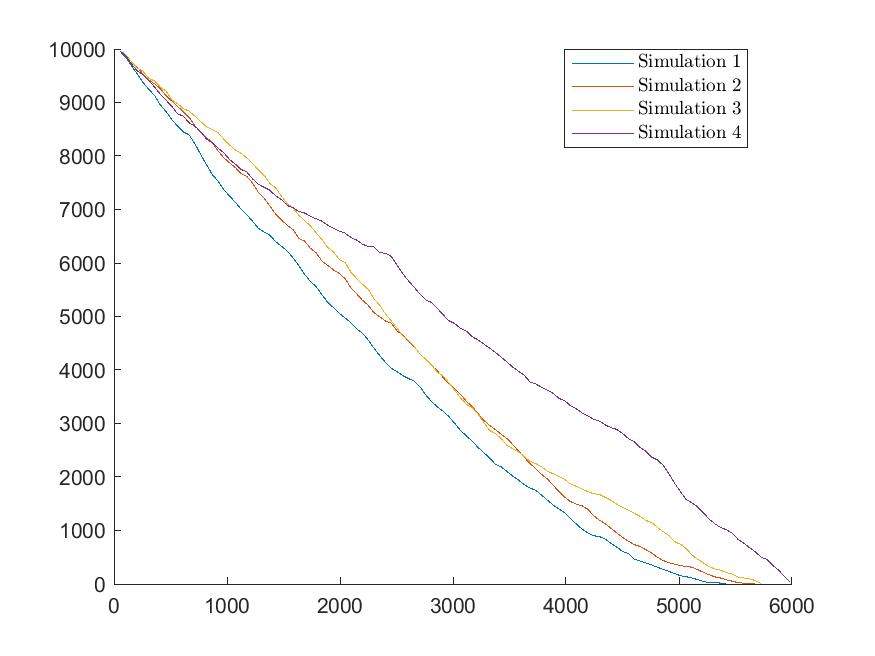
\includegraphics[width=\linewidth]{images/SS05/obj_hist.jpg}};
    \node (P0) at (0,3.5) {$J$};
    \node (P0) at (5,0) {Time (\si{\second})};
\end{scope}
\end{tikzpicture}
    \caption{Objective function over time for simulation 5}
    \label{fig:SS05_obj_hist}
\end{figure}

% % relative objective function
% \begin{figure}[h]
%     \centering
%     \begin{tikzpicture}
\begin{scope}
    \node[anchor=south west,inner sep=0] (image) at (0,0) {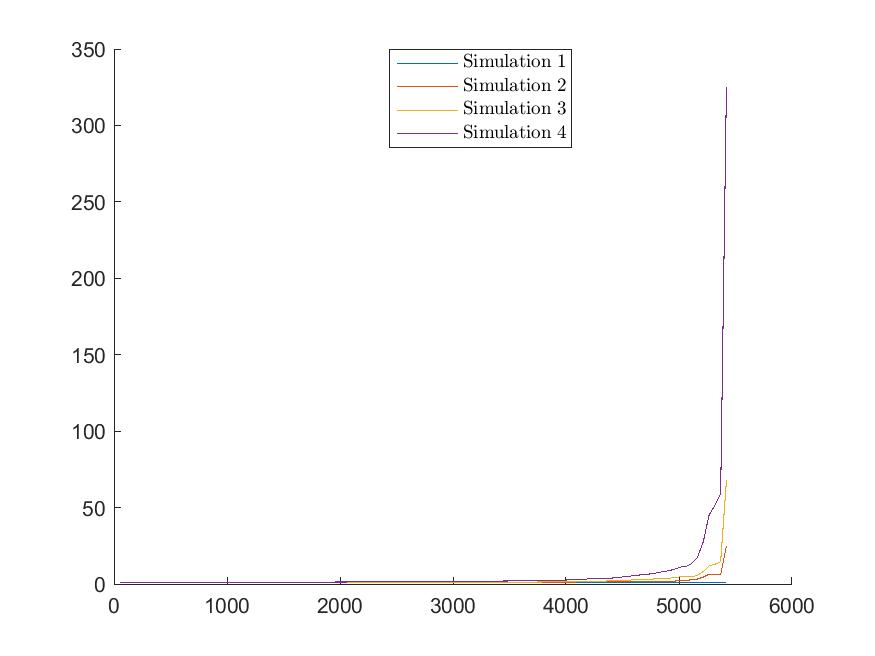
\includegraphics[width=\linewidth]{images/SS05/obj_hist_relative.jpg}};
    \node (P0) at (0,3.5) {$\frac{J_{\text{sim}}}{J_{1}}$};
    \node (P0) at (5,0) {Time (\si{\second})};
\end{scope}
\end{tikzpicture}
%     \caption{Relative performance for simulation 5}
%     \label{fig:SS05_obj_hist_rel}
% \end{figure}

% obj function sum
\begin{figure}[h]
    \centering
    \begin{tikzpicture}
\begin{scope}
    \node[anchor=south west,inner sep=0] (image) at (0,0) {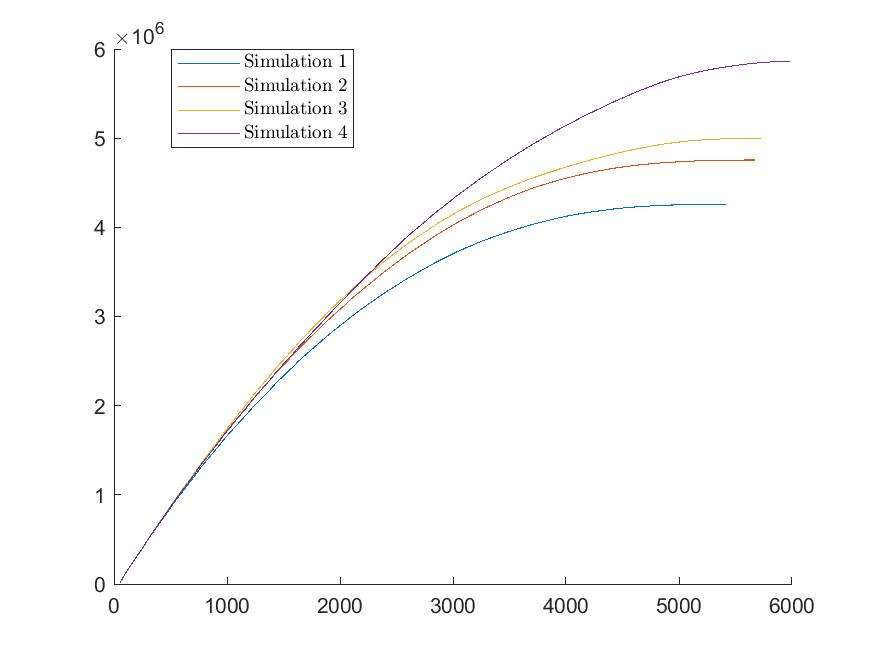
\includegraphics[width=\linewidth]{images/SS05/s_obj_hist.jpg}};
    \node (P0) at (0,3.5) {$\sum_{k_{i}=0}^{k} J$};
    \node (P0) at (5,0) {Time (\si{\second})};
\end{scope}
\end{tikzpicture}
    \caption{Objective function sum over time for simulation 5}
    \label{fig:SS05_s_obj_hist}
\end{figure}

% obj function sum
\begin{figure}[h]
    \centering
    \begin{tikzpicture}
\begin{scope}
    \node[anchor=south west,inner sep=0] (image) at (0,0) {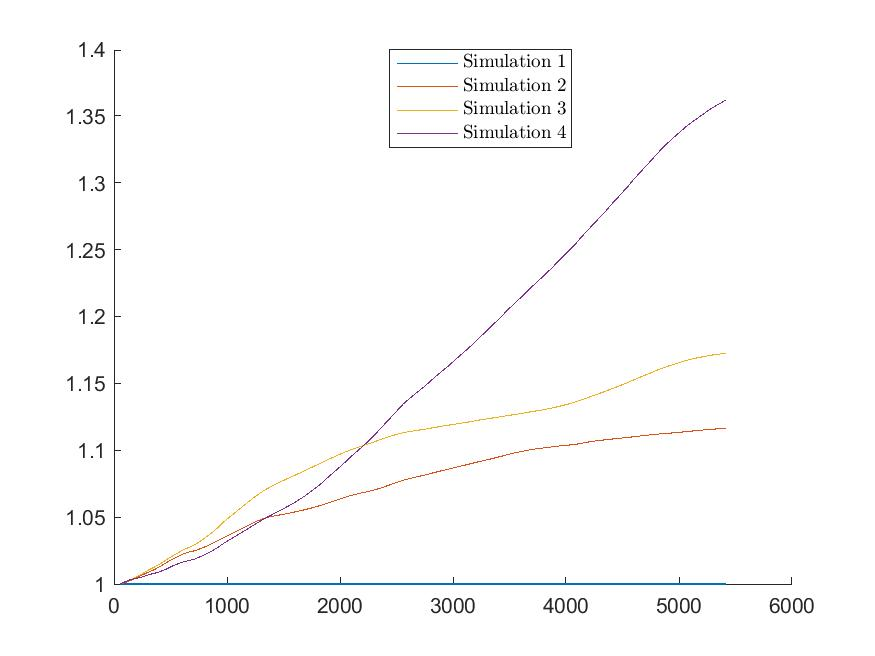
\includegraphics[width=\linewidth]{images/SS05/s_obj_hist_relative.jpg}};
    \node (P0) at (-0.5,3.5) {$\frac{\sum_{k_{i}=0}^{k} J_{\text{sim}}}{\sum_{k_{i}=0}^{k} J_{1}}$};
    \node (P0) at (5,0) {Time (\si{\second})};
\end{scope}
\end{tikzpicture}
    \caption{Relative performance for simulation 5}
    \label{fig:SS05_s_obj_rel}
\end{figure}

% % FIS output surface parameters
% \begin{figure}
%     \centering
%     \includegraphics{}
%     \caption{FIS output surface parameters for simulation 5}
%     \label{fig:SS05_fis_params}
% \end{figure}

In this simulation set, all of the simulations with the \gls{mpc} active performed worse than the control simulation.
It can be seen that the simulation with $n_{\text{fe}_{\text{max}}} = 10$ performed about \SI{10}{\percent} worse, the simulation with $n_{\text{fe}_{\text{max}}} = 40$ performed about \SI{15}{\percent} worse, and the simulation with $n_{\text{fe}_{\text{max}}} = 100$ performed about \SI{35}{\percent} worse than the control simulation.

This may partially be explained by the large number of optimisation variables required to optimise two output surfaces for each agent.
Additionally, the construction of the rule base may play a large role in the performance of the controller.

\subsection{Simulation 6 - Two Output Surfaces and Two Prediction Steps} \label{subsec:results_SS06}

% obj function by time
\begin{figure}[h]
    \centering
    \begin{tikzpicture}
\begin{scope}
    \node[anchor=south west,inner sep=0] (image) at (0,0) {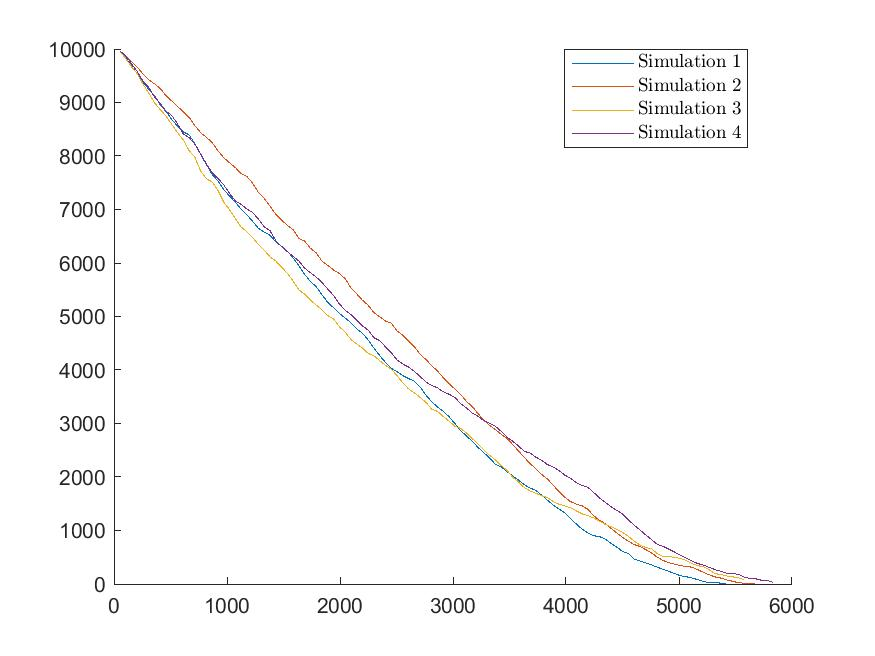
\includegraphics[width=\linewidth]{images/SS06/obj_hist.jpg}};
    \node (P0) at (0,3.5) {$J$};
    \node (P0) at (5,0) {Time (\si{\second})};
\end{scope}
\end{tikzpicture}
    \caption{Objective function over time for simulation 6}
    \label{fig:SS06_obj_hist}
\end{figure}

% % relative objective function
% \begin{figure}[h]
%     \centering
%     \begin{tikzpicture}
\begin{scope}
    \node[anchor=south west,inner sep=0] (image) at (0,0) {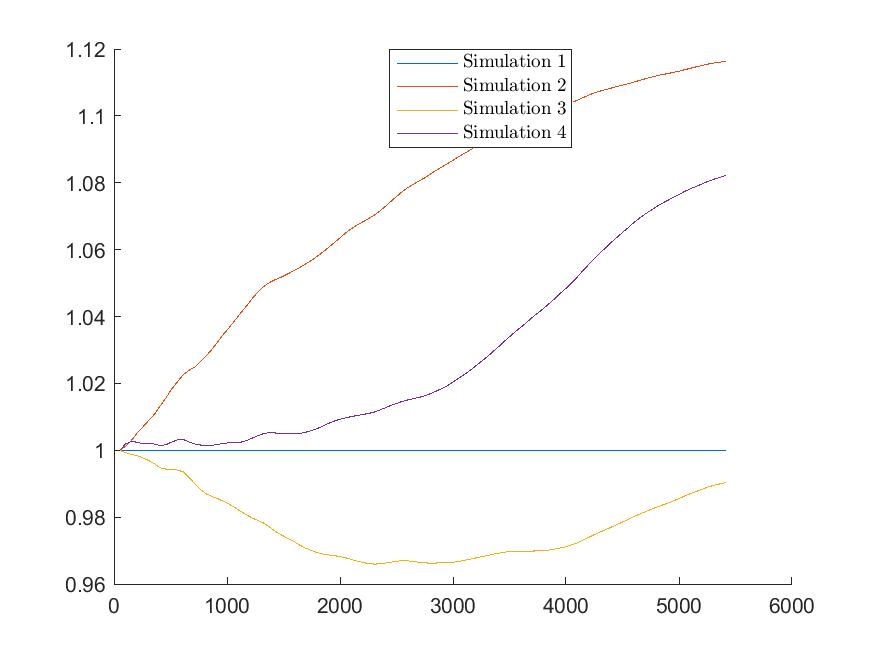
\includegraphics[width=\linewidth]{images/SS06/s_obj_hist_relative.jpg}};
    \node (P0) at (0,3.5) {$\frac{\sum_{k_{i}=0}^{k} J_{\text{sim}}}{\sum_{k_{i}=0}^{k} J_{1}}$};
    \node (P0) at (5,0) {Time (\si{\second})};
\end{scope}
\end{tikzpicture}   
%     \caption{Relative performance for simulation 6}
%     \label{fig:SS06_obj_hist_rel}
% \end{figure}

% obj function sum
\begin{figure}[h]
    \centering
    \begin{tikzpicture}
\begin{scope}
    \node[anchor=south west,inner sep=0] (image) at (0,0) {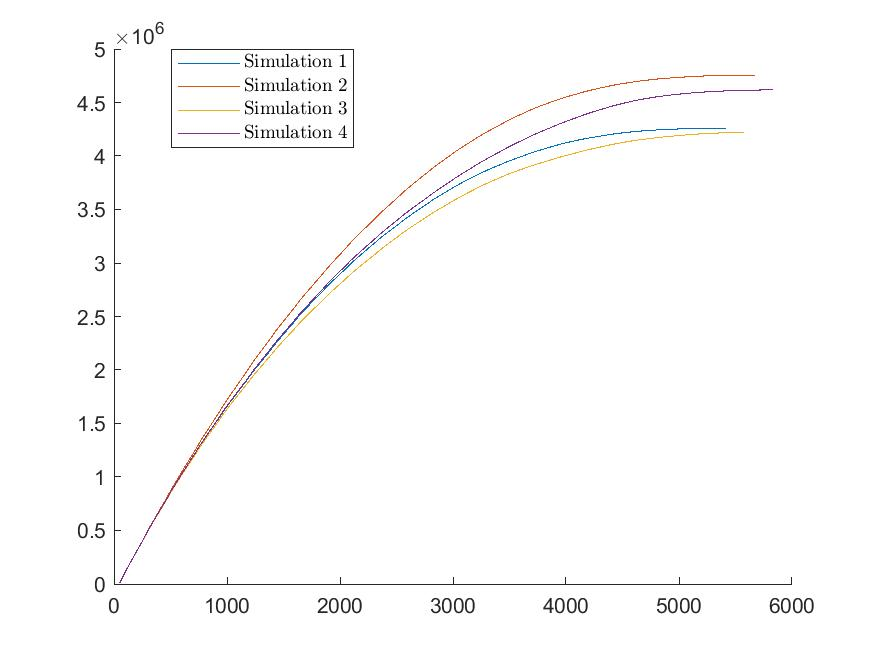
\includegraphics[width=\linewidth]{images/SS06/s_obj_hist.jpg}};
    \node (P0) at (0,3.5) {$\sum_{k_{i}=0}^{k} J$};
    \node (P0) at (5,0) {Time (\si{\second})};
\end{scope}
\end{tikzpicture}
    \caption{Objective function sum over time for simulation 6}
    \label{fig:SS06_s_obj_hist}
\end{figure}

% obj function sum
\begin{figure}[h]
    \centering
    \begin{tikzpicture}
\begin{scope}
    \node[anchor=south west,inner sep=0] (image) at (0,0) {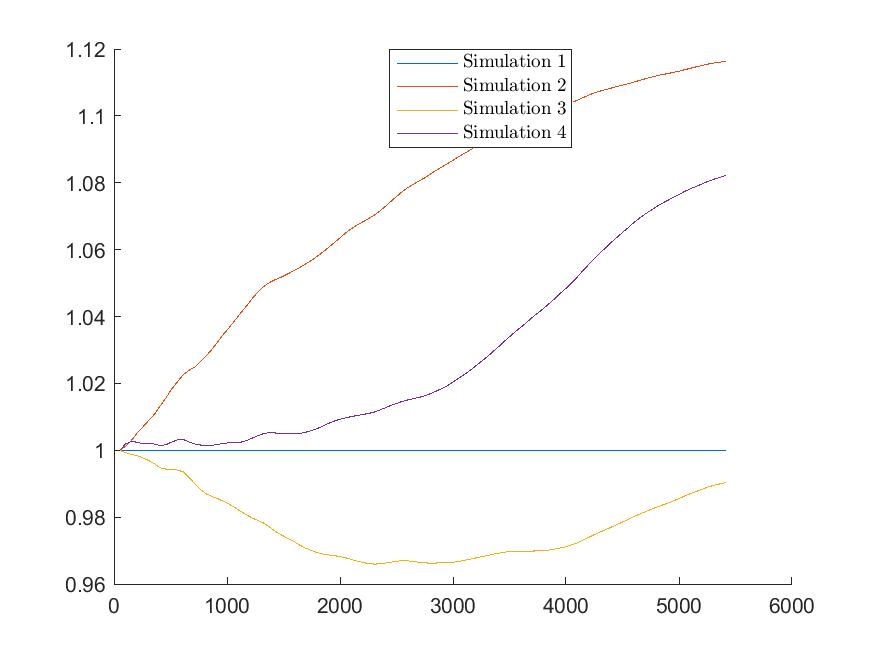
\includegraphics[width=\linewidth]{images/SS06/s_obj_hist_relative.jpg}};
    \node (P0) at (-0.5,3.5) {$\frac{\sum_{k_{i}=0}^{k} J_{\text{sim}}}{\sum_{k_{i}=0}^{k} J_{1}}$};
    \node (P0) at (5,0) {Time (\si{\second})};
\end{scope}
\end{tikzpicture}
    \caption{Relative performance for simulation 6}
    \label{fig:SS06_s_obj_rel}
\end{figure}

In this simulation, the number of prediction steps was increased to analyse whether the controller had improved performance with a larger prediction horizon.
Results for the \gls{mpc} simulations were greatly improved, with the simulation with $n_{\text{fe}_{\text{max}}} = 10$ performing about \SI{11}{\percent} worse, the simulation with $n_{\text{fe}_{\text{max}}} = 40$ performing about \SI{1}{\percent} better, and the simulation with $n_{\text{fe}_{\text{max}}} = 100$ performing about \SI{7}{\percent} worse than the control simulation despite the larger number of optimisation variables.

\subsection{Simulation 7 - Two Output Surfaces and Three Prediction Steps} \label{subsec:results_SS07}

% obj function by time
\begin{figure}[h]
    \centering
    \begin{tikzpicture}
\begin{scope}
    \node[anchor=south west,inner sep=0] (image) at (0,0) {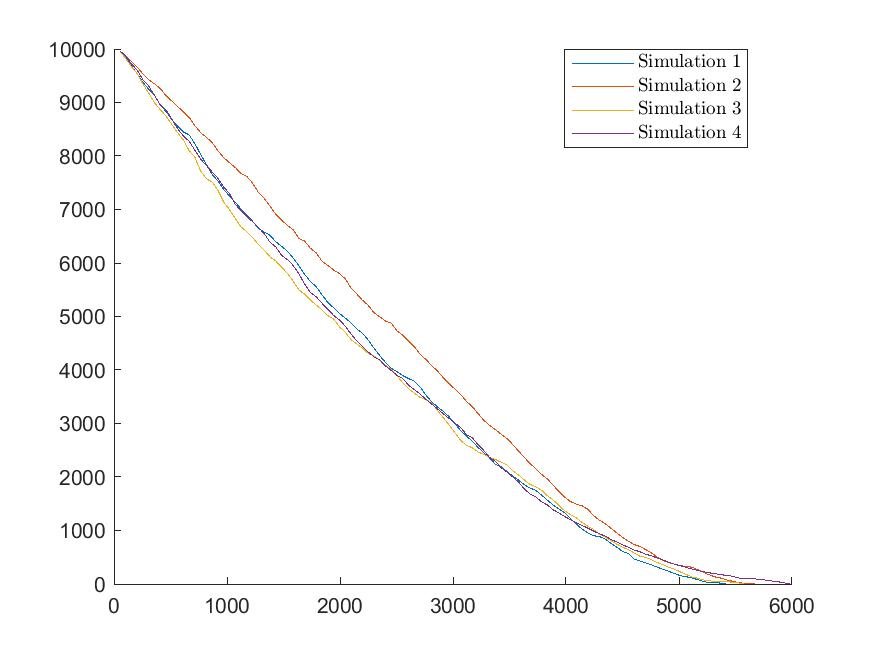
\includegraphics[width=\linewidth]{images/SS07/obj_hist.jpg}};
    \node (P0) at (0,3.5) {$J$};
    \node (P0) at (5,0) {Time (\si{\second})};
\end{scope}
\end{tikzpicture}
    \caption{Objective function over time for simulation 7}
    \label{fig:SS07_obj_hist}
\end{figure}

% % relative objective function
% \begin{figure}[h]
%     \centering
%     \begin{tikzpicture}
\begin{scope}
    \node[anchor=south west,inner sep=0] (image) at (0,0) {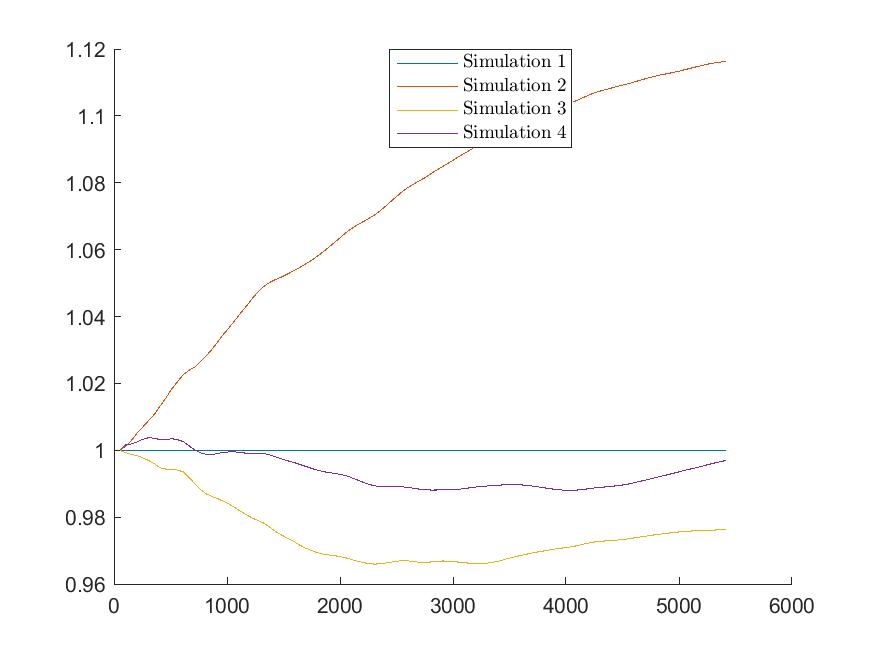
\includegraphics[width=\linewidth]{images/SS07/s_obj_hist_relative.jpg}};
    \node (P0) at (0,3.5) {$\frac{\sum_{k_{i}=0}^{k} J_{\text{sim}}}{\sum_{k_{i}=0}^{k} J_{1}}$};
    \node (P0) at (5,0) {Time (\si{\second})};
\end{scope}
\end{tikzpicture}   
%     \caption{Relative performance for simulation 7}
%     \label{fig:SS07_obj_hist_rel}
% \end{figure}

% obj function sum
\begin{figure}[h]
    \centering
    \begin{tikzpicture}
\begin{scope}
    \node[anchor=south west,inner sep=0] (image) at (0,0) {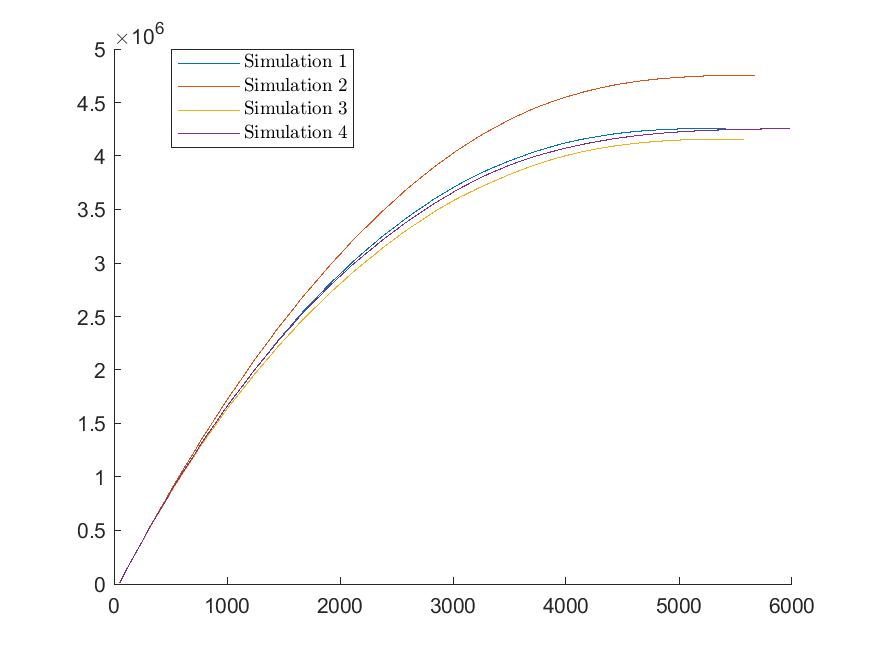
\includegraphics[width=\linewidth]{images/SS07/s_obj_hist.jpg}};
    \node (P0) at (0,3.5) {$\sum_{k_{i}=0}^{k} J$};
    \node (P0) at (5,0) {Time (\si{\second})};
\end{scope}
\end{tikzpicture}
    \caption{Objective function sum over time for simulation 7}
    \label{fig:SS07_s_obj_hist}
\end{figure}

% obj function sum
\begin{figure}[h]
    \centering
    \begin{tikzpicture}
\begin{scope}
    \node[anchor=south west,inner sep=0] (image) at (0,0) {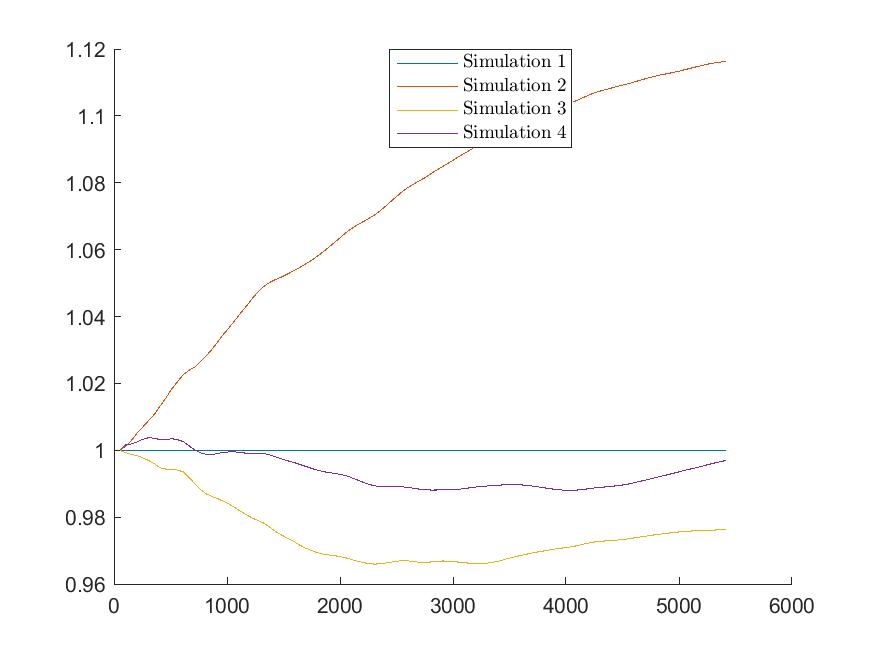
\includegraphics[width=\linewidth]{images/SS07/s_obj_hist_relative.jpg}};
    \node (P0) at (-0.5,3.5) {$\frac{\sum_{k_{i}=0}^{k} J_{\text{sim}}}{\sum_{k_{i}=0}^{k} J_{1}}$};
    \node (P0) at (5,0) {Time (\si{\second})};
\end{scope}
\end{tikzpicture}
    \caption{Relative performance for simulation 7}
    \label{fig:SS07_s_obj_rel}
\end{figure}

In this simulation, the number of prediction steps was once again increased to analyse whether the controller had improved performance with a larger prediction horizon.
Results for the \gls{mpc} simulations were further improved, with the simulation with $n_{\text{fe}_{\text{max}}} = 10$ performing about \SI{11}{\percent} worse, the simulation with $n_{\text{fe}_{\text{max}}} = 40$ performing about \SI{2}{\percent} better, and the simulation with $n_{\text{fe}_{\text{max}}} = 100$ performing <\SI{1}{\percent} better than the control simulation despite the larger number of optimisation variables.

\subsection{Simulation 8 - Two Output Surfaces and Three Prediction Steps with Extended Prediction Time Step} \label{subsec:results_SS08}

% obj function by time
\begin{figure}[h]
    \centering
    \begin{tikzpicture}
\begin{scope}
    \node[anchor=south west,inner sep=0] (image) at (0,0) {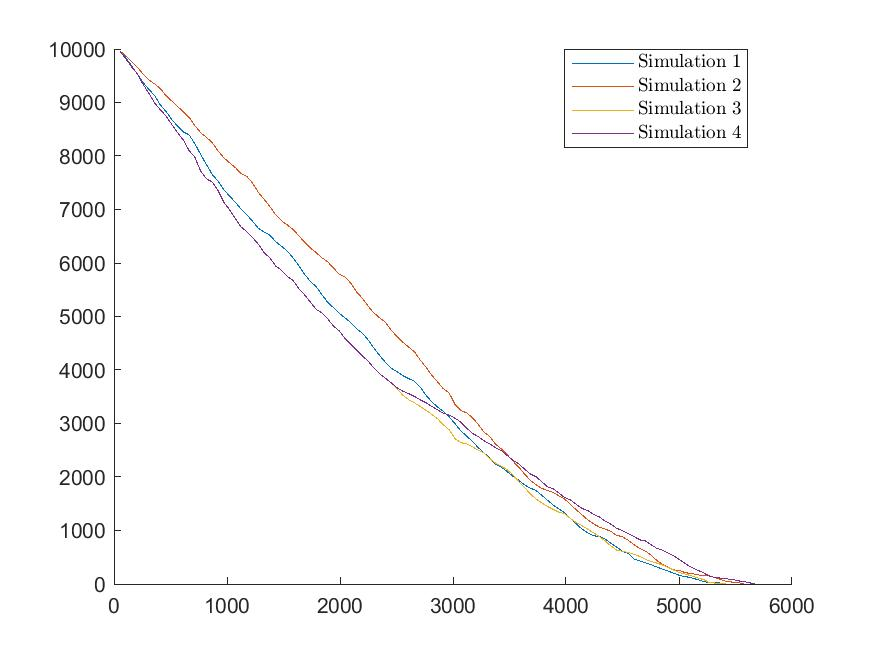
\includegraphics[width=\linewidth]{images/SS08/obj_hist.jpg}};
    \node (P0) at (0,3.5) {$J$};
    \node (P0) at (5,0) {Time (\si{\second})};
\end{scope}
\end{tikzpicture}
    \caption{Objective function over time for simulation 8}
    \label{fig:SS08_obj_hist}
\end{figure}

% % relative objective function
% \begin{figure}[h]
%     \centering
%     \begin{tikzpicture}
\begin{scope}
    \node[anchor=south west,inner sep=0] (image) at (0,0) {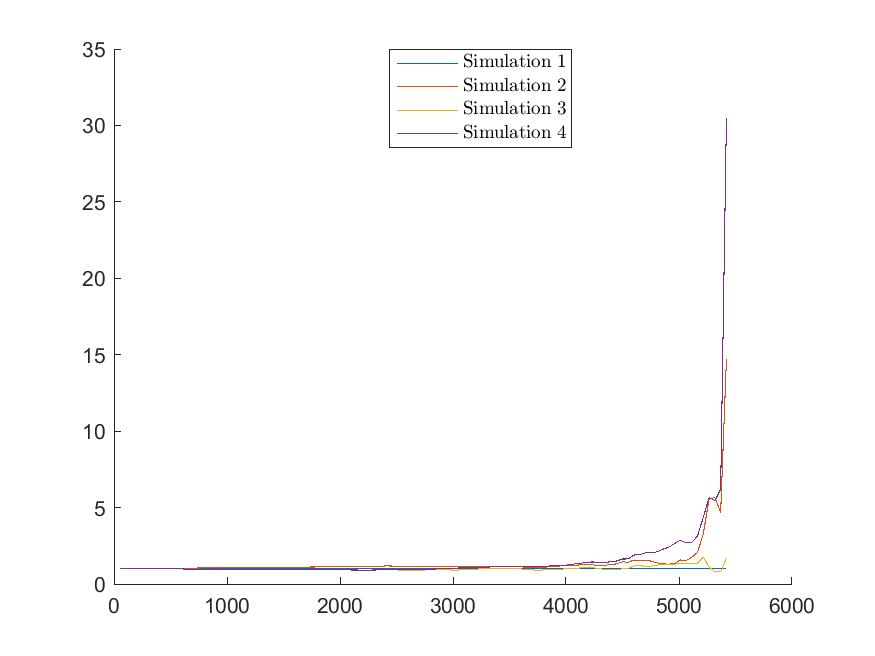
\includegraphics[width=\linewidth]{images/SS08/obj_hist_relative.jpg}};
    \node (P0) at (0,3.5) {$\frac{J_{\text{sim}}}{J_{1}}$};
    \node (P0) at (5,0) {Time (\si{\second})};
\end{scope}
\end{tikzpicture}
%     \caption{Relative performance for simulation 8}
%     \label{fig:SS08_obj_hist_rel}
% \end{figure}

% obj function sum
\begin{figure}[h]
    \centering
    \begin{tikzpicture}
\begin{scope}
    \node[anchor=south west,inner sep=0] (image) at (0,0) {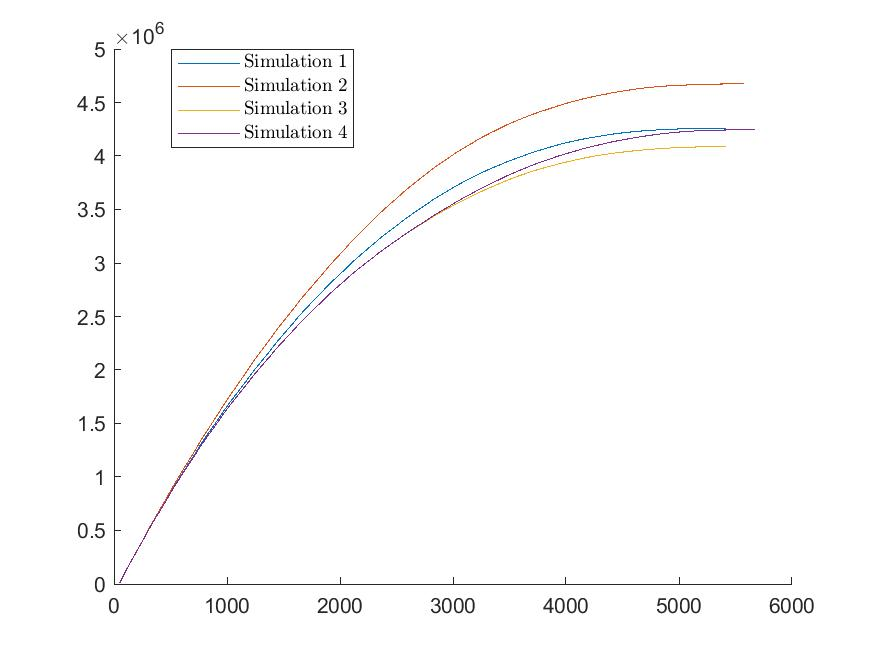
\includegraphics[width=\linewidth]{images/SS08/s_obj_hist.jpg}};
    \node (P0) at (0,3.5) {$\sum_{k_{i}=0}^{k} J$};
    \node (P0) at (5,0) {Time (\si{\second})};
\end{scope}
\end{tikzpicture}
    \caption{Objective function sum over time for simulation 8}
    \label{fig:SS08_s_obj_hist}
\end{figure}

% obj function sum
\begin{figure}[h]
    \centering
    \begin{tikzpicture}
\begin{scope}
    \node[anchor=south west,inner sep=0] (image) at (0,0) {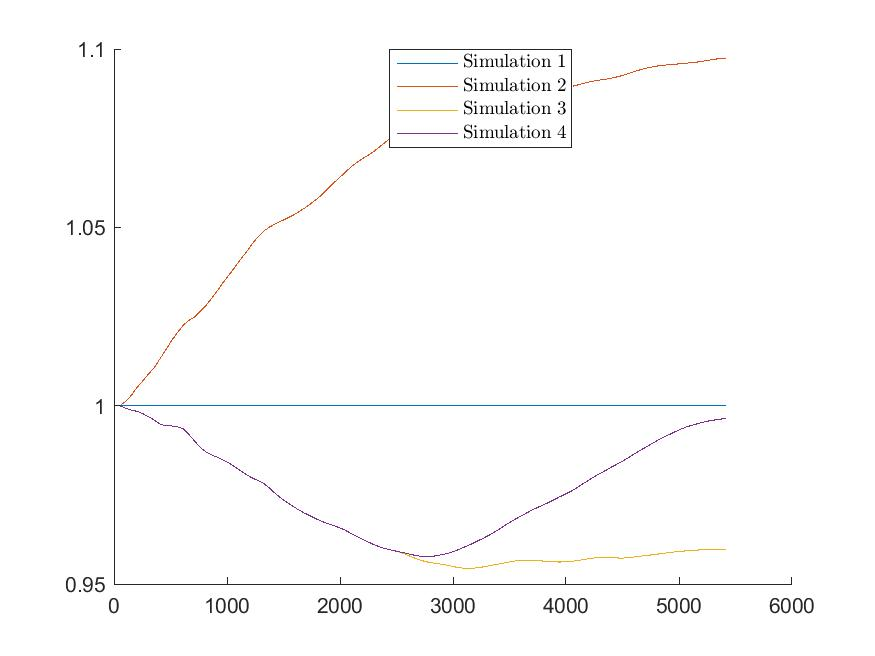
\includegraphics[width=\linewidth]{images/SS08/s_obj_hist_relative.jpg}};
    \node (P0) at (-0.5,3.5) {$\frac{\sum_{k_{i}=0}^{k} J_{\text{sim}}}{\sum_{k_{i}=0}^{k} J_{1}}$};
    \node (P0) at (5,0) {Time (\si{\second})};
\end{scope}
\end{tikzpicture}
    \caption{Relative performance for simulation 8}
    \label{fig:SS08_s_obj_rel}
\end{figure}

In this simulation, the size of the prediction step was increased to \SI{2880}{\second}.
Compared to the previous simulation, the controller with $n_{\text{fe}_{\text{max}}} = 10$ had similar performance, about \SI{10}{\percent} worse than the control simulation, while the controller with $n_{\text{fe}_{\text{max}}} = 40$ performed about \SI{4}{\percent} better and the simulation with $n_{\text{fe}_{\text{max}}} = 100$ performed \SI{1}{\percent} better than the control simulation.

This may not reflect how the controller would perform in reality, as using probability-based models for prediction would compound prediction errors over time and could result in worse performance than a smaller prediction step.
It is likely that there is a 'sweet spot' for the prediction horizon, where the errors in prediction are balanced out by the advantages offered by the insight of the prediction horizon.

\section{Conclusion}\label{sec:conclusion}

\section{Recommendations}\label{sec:recommendations}

% Moved from "assumptions" sections:
% Firstly, the environment is divided into equal sized squares which are scanned individually.
% In a real disaster environment, it would be more optimal to divide the environment into polyhedral shapes which would be most efficient to scan at the same time.
% For instance, buildings would be kept in the same cell and would be scanned all at once instead of split into multiple cells.
% In reality, the disaster environment would be a \gls{3d} area with many obstacles and require obstacle avoidance path planning.
% In terms of a-priori data, it is assumed that the disaster environment is uniformly affected and building coverage provides a good indicator of the location of victims.

There are plenty of possibilities to extend upon the work achieved in this project.
In this section, recommendations are given for the additional work that would be necessary for implementation of the proposed controller in a real-life system.
Recommendations are categorised according to the various aspects of the simulation which require further work.

\subsection{Modelling}

Further work on the modelling used in the simulation is recommended with the goal that the mathematical models used in the simulation represent to an acceptable deal of accuracy the physical models that they represent.

\subsubsection{Agent Modelling}
The agent model used in this project is an abstract discrete 2D model with simple dynamics for movement and scanning.
A more advanced model could choose a type of agent to model, for instance quadcopter \gls{uav}s, and include 3D dynamics modelling (aerodynamics, structure, etc.), sensor modelling (camera, infrared, cellular network communications, etc), and electronics modelling (battery, etc).

\subsubsection{Environment Modelling}
The environment model used in the simulation is a simple discrete 2D top-down model of a disaster environment and includes static models for wind and building coverage, and a cellular automata-based dynamic model, for fire.
Further work could develop a 3D environment model based on LIDAR datasets of disaster environments, 3D dynamic modelling of wind, and physics-based 3D modelling of fire.
Additional models could also be implemented in the simulation if they could have relevance to the operation of the system, such as smoke, victim location, search team, charging stations, building damage, and so on.

\subsection{Controller Design}

This work has established a functional controller structure for autonomous search and rescue systems.
Further work could focus on improving the performance and efficiency of this structure.

\subsubsection{Path Planning Controller}
If 3D simulation models are implemented, the path planning controller should also operate with 3D waypoints.
Further changes could include obstacle avoidance implementation for navigating a 3D environment and discretisation of the environment into polygonal search cells, instead of dividing it into a grid, according to the fastest search patterns - for example, identifying individual buildings as separate search cells, as it would be most efficient to scan one building all at the same time.
The path planning controller could also be a focus of computational efficiency improvements.
For example, currently the path planning controller will calculate the attraction of all unscanned cells at each path planning time step, whereas it could potentially analyse a constant \textit{n} closest cells with negligible drop in performance.

\subsubsection{\gls{mpc} Design}

Studies focusing on the \gls{mpc} design could look at the optimal choice of objective function for the \gls{mpc} module, the optimal solver configuration for the optimisation, the optimal setup of the \gls{mpc} (prediction horizon, etc), and moving the \gls{mpc} model to a probability-based model, as in a real application the system would not have access to perfect information as is assumed in this project.
The \gls{mpc} solver could also implement multi-objective optimisation to consider other important objectives of the agents, such as battery life limitations and recharging, etc.

\subsubsection{\gls{fis} Design}
Further studies could focus on the design of the \gls{fis} by analysing the optimal combinations of inputs, number and shape of membership functions, number of output surfaces, and design of the rule base.
Potential new inputs for the \gls{fis} could include different methods to categorise risk to victims due to dynamic environment variables, such as the \textit{downwind time} used in this project.
This line of research should also focus on determining a balance between the complexity of the \gls{fis} and the computational power available for the \gls{fis} in a real-world application.

\subsection{Validation}

Various work would be necessary to validate the system for real-world application.

\subsubsection{Scaled Experiment}

After satisfactory simulation results with appropriately accurate modelling, a scaled experiment of the system should be conducted in a controlled environment to determine any inconsistencies between simulation and reality.
  
\subsubsection{Scalability}

The scalability of the system should be analysed through simulation or experimentation to determine any limitations on the operation of the system, as a real-life application may require a large number of agents depending upon the scale of the disaster environment.

\subsubsection{Robustness}

The system should be robust to disruptions and disturbances in the system, such as losing agents to environmental hazards, erroneous measurements in the system, and so on.

\subsubsection{System Design} 
Finally, the work in this thesis would compose one small part of the overall search and rescue operations, and should integrate seamlessly into the existing search and rescue operations structure.
For example, this would require interfacing between the autonomous search and rescue system and linked systems such as rescue personnel and sources of a-priori data (satellite imagery, etc).
The potential for further work in this area is near limitless, but a suggested first avenue of research would be in the full system design of a search and rescue system implementing the work in this project.

\subsection{Final Note}

This project has established the basis for an autonomous search and rescue system using waypoint-based model predictive fuzzy control.
There is still a large amount of research required for a functional real-life system, but with further research in the areas identified in this section it could become a reality.

% Glossary
% \printglossary

% Bibliography
\bibliography{bibliography} 
\bibliographystyle{ieeetr}

\end{document}

%% ERRATA
% % Original notation
% \begin{equation}
%     p(t_{ckl}) = 
%     \begin{cases} 
%         \frac{4}{t_{b} - t_{i}} t_{ckl} + \frac{0.2 t_{b} - 4.2 t_{i}}{{1}} & t_{i} \leq t_{ckl} \leq \frac{t_{b} - t_{i}}{5} + t_{i} \\
%         \frac{5}{4 (t_{b} - t_{i}) } (-t_{ckl} + t_{b} ) & \frac{t_{b} - t_{i}}{5} + t_{i} \leq t_{ckl} \leq t_{b} \\
%     \end{cases}
% \end{equation}

% To test how the objective function responds to variations in the output surface parameters, an \textit{objective function sensitivity test} was designed.
% This test is run at each \gls{mpc} time step.
% In this test, the objective function for the \gls{mpc} prediction is evaluated for a predefined range of output surface parameters.

% \subsection{Time Sensitivity}

% In this test, the \gls{mpc} objective function was evaluated over the course of a simulation.
% The results are given in figure \ref{fig:objSensitivityTime}.

% \begin{figure}
%     \centering
%     \includegraphics[width=\linewidth]{images/tests/objSensitivityTime.jpg}
%     \caption{Time Sensitivity of \gls{mpc} Objective Function}
%     \label{fig:objSensitivityTime}
% \end{figure}

% It can be seen that the objective function decreases over the duration of the simulation, as more cells are scanned.
% This indicates that the objective function is a good indication of the performance of the search and rescue system, and that minimising it will lead to improved performance.

% \subsection{Sensitivity Test 1} \label{subsec:sensitivityTest1}

% The setup for \textit{sensitivity test 1} is given in table \ref{tab:objSensitivityTest1}.
% The sensitivity test is performed for all combinations of output surface parameters and the simulation is terminated at $n_{\text{MPC}} = 5$.
% The parameter ranges are extended to $\pm 0.2$ their initial value.

% \begin{table}[]
%     \centering
%     \caption{Objective Function Sensitivity Test 1}
%     \label{tab:objSensitivityTest1}
%     \begin{tabular}{r|l}
%         Parameter   & Range \\
%         $p1$        & [-0.8 -0.9 -1.0 -1.1 -1.2] \\
%         $p2$        & [12800 14400 16000 17600 19200] \\
%         $p3$        & 1 \\
%         $p4$        & 1 \\
%     \end{tabular}
% \end{table}

% The results for the sensitivity test at $n_{MPC} = 1$ are shown in figure \ref{fig:testSensitivityObj1}.
% It can be seen that the objective function is the same for all combinations of the output parameter ranges defined in the table.

% \begin{figure}
%     \centering
%     \includegraphics[width=\linewidth]{images/tests/sensitivityTest1MPCStep1.jpg}
%     \caption{Objective Function Sensitivity Test 1 at $n_{MPC} = 1$}
%      \label{fig:testSensitivityObj1}
% \end{figure}

% \subsection{Sensitivity Test 2} \label{subsec:sensitivityTest2}

% In case the originally provided ranges were not large enough, a second \gls{mpc} objective function sensitivity test was designed.
% The setup for \textit{sensitivity test 2} is given in table \ref{tab:objSensitivityTest2}, where both parameter ranges are extended to $\pm 0.4$ their initial value.

% \begin{table}[]
%     \centering
%     \caption{Objective Function Sensitivity Test 2}
%     \label{tab:objSensitivityTest2}
%     \begin{tabular}{r|l}
%         Parameter   & Range \\
%         $p1$        & [-0.6 -0.8 -1.0 -1.2 -1.4] \\
%         $p2$        & [9600 12800 16000 19200 22400] \\
%         $p3$        & 1 \\
%         $p4$        & 1 \\
%     \end{tabular}
% \end{table}

% \begin{figure}
%     \centering
%     \includegraphics[width=\linewidth]{images/tests/sensitivityTest2MPCStep1.jpg}
%     \caption{Objective Function Sensitivity Test 2 at $n_{MPC} = 1$}
%     \label{fig:testSensitivityObj2}
% \end{figure}

% Once again, The results for this sensitivity test were that the objective function is the same for all combinations of the output parameter ranges.

% \subsection{Sensitivity Test Discussion}

% Clearly, in the simulation the objective function is not sensitive to changes in the output surface parameters.
% The may be due to the design of the \gls{fis}, which has inputs of very different magnitudes, for instance the range of \textit{priority} $ = [0~1]$ while the range of \textit{time} $ = [0~16000]$.
% This large range is required for the \textit{time} input as it can reach very large values when evaluating cells which are far from the agents, but the time values of interest are likely to only be the nearby ones which have a greater attraction.

% Two possible solutions to this are \textit{multiple output surfaces} or \textit{normalisation}.

% \textit{Multiple output surfaces} could be used to make the attraction with relation to time constant above a certain value, increasing the sensitivity of attraction to lower values of the time input.

% For \textit{normalisation}, regression techniques could be applied, particularly \textit{logistic regression}, shown in figure \ref{}, which compresses numbers on both ends of the range.
% A combination of linear regression and logistic regression could be applied so that only numbers on the high end of the \textit{time} input range are compressed.

% \begin{figure}
%     \centering
%     \includegraphics[width=\linewidth]{images/other/regressionMethods.jpeg}
%     \caption{Regression Methods \cite{prabhakaran_2019}}
%     \label{fig:regressionMethods}
% \end{figure}

% \subsection{Scaling Test}
% % Check variable values.
% In response to this results of the \textit{sensitivity} test, a \textit{scaling} test was designed.
% In this test, a simulation was run for the first 10 \gls{mpc} time steps and the values of important simulation variables were recorded.
% These were the \textit{objective function components}, $P_{\text{bo}}$ and $P_{\text{fo}}$, and the \textit{\gls{fis} components}, $\textit{att}$, $t_{\text{travel}}$, $t_{\text{dw}}$, and $P$.

% \begin{figure}
%     \centering
%     \includegraphics[width=\linewidth]{images/tests/scalingObj.jpg}
%     \caption{Objective Function Components Scaling Test}
%     \label{fig:testScalingObj}
% \end{figure}

% For the \textit{objective function sensitivity test}, $201,000$ data points were recorded, shown in figure \ref{fig:testScalingObj}.
% It can be seen that many of the points are overlapping, with only a few values of each component appearing and a limited number of combinations.
% This may indicate that the evaluation of the priority is not perfect as it may not account exactly for the different variables it depends on.
% However, there is no apparent issue with scaling. 

% \begin{figure*}
%     \centering
%     \includegraphics[width=\linewidth]{images/tests/scalingFis.jpg}
%     \caption{FIS Components Scaling Test}
%     \label{fig:testScalingFIS}
% \end{figure*}

% For the \textit{\gls{fis} sensitivity test}, $127,283$ data points were recorded, shown in figure \ref{fig:testScalingFIS}.
% It can be seen that the \textit{priority} input does not change at all during the simulation.
% This is due to a problem with the calculation of priority and will need to be fixed.
% Several artefacts can be seen at the top of the $t_{dw}$ scale.
% These are introduced by a bug in the calculation method.The range for the $t_\textit{nextcell}$ input is also far larger than the other inputs, and the \textit{attraction} for each cell is clearly far more dependent on this input than the other inputs combined.
% The issue with optimisations not working and the objective function not changing with output surface parameters can therefore be traced back to this problem.

% The proposed solution is to implement correct calculation of the \textit{priority} input, fix the artefact bug in the $t_{dw}$ calculation, implement normalisation on the $t_\textit{nextcell}$ to restrict its range to $[0~1]$, and to ensure that the attraction is similarly dependent on all three inputs.

% \subsection{Normalisation Tests}

% % Objective function
% Figure \ref{fig:obj_hist_ut} shows the objective function over the course of the simulation.

% \begin{figure}
%     \centering
%     \includegraphics[width=\linewidth]{images/sim_untuned/obj_hist.jpg}
%     \caption{Objective Function History Plot}
%     \label{fig:obj_hist_ut}
% \end{figure}

% % Objective function sum
% Figure \ref{fig:s_obj_hist_ut} shows the accumulated objective function over the course of the simulation.

% \begin{figure}
%     \centering
%     \includegraphics[width=\linewidth]{images/sim_untuned/s_obj_hist.jpg}
%     \caption{Objective Function Sum History Plot}
%     \label{fig:s_obj_hist_ut}
% \end{figure}

% Figure \ref{fig:paths_ut} shows the paths taken by the agents over the course of the simulation.

% % Paths
% \begin{figure}
%     \centering
%     \includegraphics[width=\linewidth]{images/sim_untuned/UAV_loc_hist.jpg}
%     \caption{UAV Paths}
%     \label{fig:paths_ut}
% \end{figure}

